\documentclass[12pt,oneside,a4paper,parskip,pointlessnumbers]{scrbook}
\usepackage[utf8]{inputenc}
\usepackage{csquotes}
\usepackage[ngerman]{babel}
\usepackage{floatflt}
\usepackage{subfigure}
\usepackage[pdftex]{graphicx}
\usepackage{wrapfig}
\usepackage[hidelinks]{hyperref}
\usepackage{color}
\usepackage{amssymb}
\usepackage{textcomp}
\usepackage{nicefrac}
\usepackage{scrhack}
\usepackage{pdfpages}
\usepackage{float}
\usepackage{pdflscape}
\usepackage{subfigure}
\usepackage{pdfpages}
\usepackage[verbose]{placeins}
\usepackage[headsepline,plainfootsepline]{scrlayer-scrpage}
\usepackage{listings}
%\usepackage{xcolor}
\usepackage[table]{xcolor}
%\usepackage{color}
\usepackage{caption}
\usepackage{subfigure}
\usepackage{epstopdf}
\usepackage{longtable}
\usepackage{setspace}
\usepackage{booktabs}
\usepackage[style=numeric,sorting=none,backend=bibtex]{biblatex}
\bibliography{sources}


%%%%%%%%%%%%%%%%%%%
%% definitions
%%%%%%%%%%%%%%%%%%%
\def\BaAuthor{Henning Janning}
\def\BaTitle{Evaluation von Web Application Vulnerability Scannern}
\def\BaSupervisorOne{Prof. Dr.-Ing. Andreas Mayer}
\def\BaSupervisorTwo{Susanne Steuer, (M.Sc.) }
\def\BaDeadline{04.04.2019}
\def\MatNr{192972}

\hypersetup{
pdfauthor={\BaAuthor},
pdftitle={\BaTitle},
pdfsubject={Subject},
pdfkeywords={Keywords}
}

%%%%%%%%%%%%%%%%%%%
%% configs to include
%%%%%%%%%%%%%%%%%%%
\colorlet{punct}{red!60!black}
\definecolor{background}{HTML}{EEEEEE}
\definecolor{delim}{RGB}{20,105,176}
\colorlet{numb}{magenta!60!black}

\definecolor{gray}{rgb}{0.4,0.4,0.4}
\definecolor{darkblue}{rgb}{0.0,0.0,0.6}
\definecolor{cyan}{rgb}{0.0,0.6,0.6}

\definecolor{pblue}{rgb}{0.13,0.13,1}
\definecolor{pgreen}{rgb}{0,0.5,0}
\definecolor{pred}{rgb}{0.9,0,0}
\definecolor{pgrey}{rgb}{0.46,0.45,0.48}

\lstset{
  basicstyle=\ttfamily,
  columns=fullflexible,
  showstringspaces=false,
  commentstyle=\color{gray}\upshape
  linewidth=\textwidth
}

\lstdefinelanguage{json}{
    basicstyle=\normalfont\ttfamily,
    numbers=left,
    numberstyle=\scriptsize,
    stepnumber=1,
    numbersep=8pt,
    showstringspaces=false,
    breaklines=true,
    backgroundcolor=\color{background},
    literate=
     *{0}{{{\color{numb}0}}}{1}
      {1}{{{\color{numb}1}}}{1}
      {2}{{{\color{numb}2}}}{1}
      {3}{{{\color{numb}3}}}{1}
      {4}{{{\color{numb}4}}}{1}
      {5}{{{\color{numb}5}}}{1}
      {6}{{{\color{numb}6}}}{1}
      {7}{{{\color{numb}7}}}{1}
      {8}{{{\color{numb}8}}}{1}
      {9}{{{\color{numb}9}}}{1}
      {:}{{{\color{punct}{:}}}}{1}
      {,}{{{\color{punct}{,}}}}{1}
      {\{}{{{\color{delim}{\{}}}}{1}
      {\}}{{{\color{delim}{\}}}}}{1}
      {[}{{{\color{delim}{[}}}}{1}
      {]}{{{\color{delim}{]}}}}{1},
}

\lstset{language=xml,
  morestring=[b]",
  morestring=[s]{>}{<},
  morecomment=[s]{<?}{?>},
  stringstyle=\color{black},
  numbers=left,
  numberstyle=\scriptsize,
  stepnumber=1,
  numbersep=8pt,
  identifierstyle=\color{darkblue},
  keywordstyle=\color{cyan},
  backgroundcolor=\color{background},
  morekeywords={xmlns,version,type}% list your attributes here
}

\lstset{language=Java,
  showspaces=false,
  showtabs=false,
  tabsize=4,
  breaklines=true,
  keepspaces=true,
  numbers=left,
  numberstyle=\scriptsize,
  stepnumber=1,
  numbersep=8pt,
  showstringspaces=false,
  breakatwhitespace=true,
  commentstyle=\color{pgreen},
  keywordstyle=\color{pblue},
  stringstyle=\color{pred},
  basicstyle=\ttfamily,
  backgroundcolor=\color{background},
%  moredelim=[il][\textcolor{pgrey}]{$$},
%  moredelim=[is][\textcolor{pgrey}]{\%\%}{\%\%}
}




\begin{document}

%%%%%%%%%%%%%%%%%%%
%% Titelseite
%%%%%%%%%%%%%%%%%%%


\frontmatter
\titlehead{%  {\centering Seitenkopf}
  {Hochschule Heilbronn\\
   Fakultät für Informatik}}
\subject{Bachelorarbeit}
\title{\BaTitle\\[15mm]}
\subtitle{\normalsize{vorgelegt an der Hochschule Heilbronn, Fakultät für Informatik zum Abschluss eines Studiums im Studiengang Angewandte Informatik}}
\author{\BaAuthor\\
\normalsize{Matrikelnummer: \MatNr}}
\bigskip
\date{\normalsize{Eingereicht am: \BaDeadline}}
\publishers{
  \normalsize{Erstpr\"{u}fer: \BaSupervisorOne}\\
  \normalsize{Zweitpr\"{u}ferin: \BaSupervisorTwo}\\
}

%\uppertitleback{ }
%\lowertitleback{ }

\maketitle


%%%%%%%%%%%%%%%%%%%
%% abstract
%%%%%%%%%%%%%%%%%%%

\section*{Zusammenfassung}

In dieser Arbeit werden aktuelle Web Vulnerability Scanner (WVS) auf ihren Umfang und ihre Tauglichkeit überprüft und verglichen. Jeder WVS wird an verschiedenen Web-Seiten getestet, die absichtlich eingebaute Schwachstellen haben, wie z.B. Juice-Shop oder Damn Vulnerable Web Application. Kriterien für die Bewertung der Tools sind die Anzahl der gefundenen Schwachstellen, Anzahl der False Positives und die daraus resultierende Trefferquote. Zudem fließen subjektive Eindrücke wie Handhabung oder intuitive Bedienung in die Bewertung mit ein.

\section*{Abstract}
TODO


\setcounter{secnumdepth}{3}
\setcounter{tocdepth}{3}
\tableofcontents

\listoffigures
\addcontentsline{toc}{chapter}{Abbildungsverzeichnis}

\listoftables
\addcontentsline{toc}{chapter}{Tabellenverzeichnis}

\mainmatter

\chapter{Einführung}\label{ch:intro}
In den letzten zwei Jahrzehnten hat sich das World Wide Web von einem reinen Informationsspeicher in eine Plattform mit hochfunktionalen Anwendungen verwandelt, die nicht nur sensible Daten verarbeiten sondern auch  Aktionen durchführen, die einflussreiche Auswirkungen auf die reale Welt haben.
Mit jeder Weiterentwicklung bringen Webanwendungen neue Sicherheitslücken mit sich und so verändern sich auch die Art und die Anzahl der am häufigsten auftretenden Fehler. Es gibt Angriffe auf Schwachstellen, die bei der Entwicklung der Webanwendungen noch nicht bekannt waren und daher nicht berücksichtigt wurden, andere Attacken haben an Bedeutung verloren, da das Bewusstsein für sie gestiegen ist oder aufgrund von Verbesserungen der Web-Browser Software. Neue Technologien bergen jedoch auch immer das Risiko von neuen Sicherheitslücken und so ist ``...in gewissem Maße die Sicherheit von Webanwendungen heute das bedeutendste Schlachtfeld zwischen Angreifern und solchen, die Daten schützen und Computerressourcen verteidigen müssen, und dies wird wahrscheinlich auf absehbare Zeit so bleiben.'' \cite[S.6]{handbook}

\begin{figure}[htb!]
  \centering
    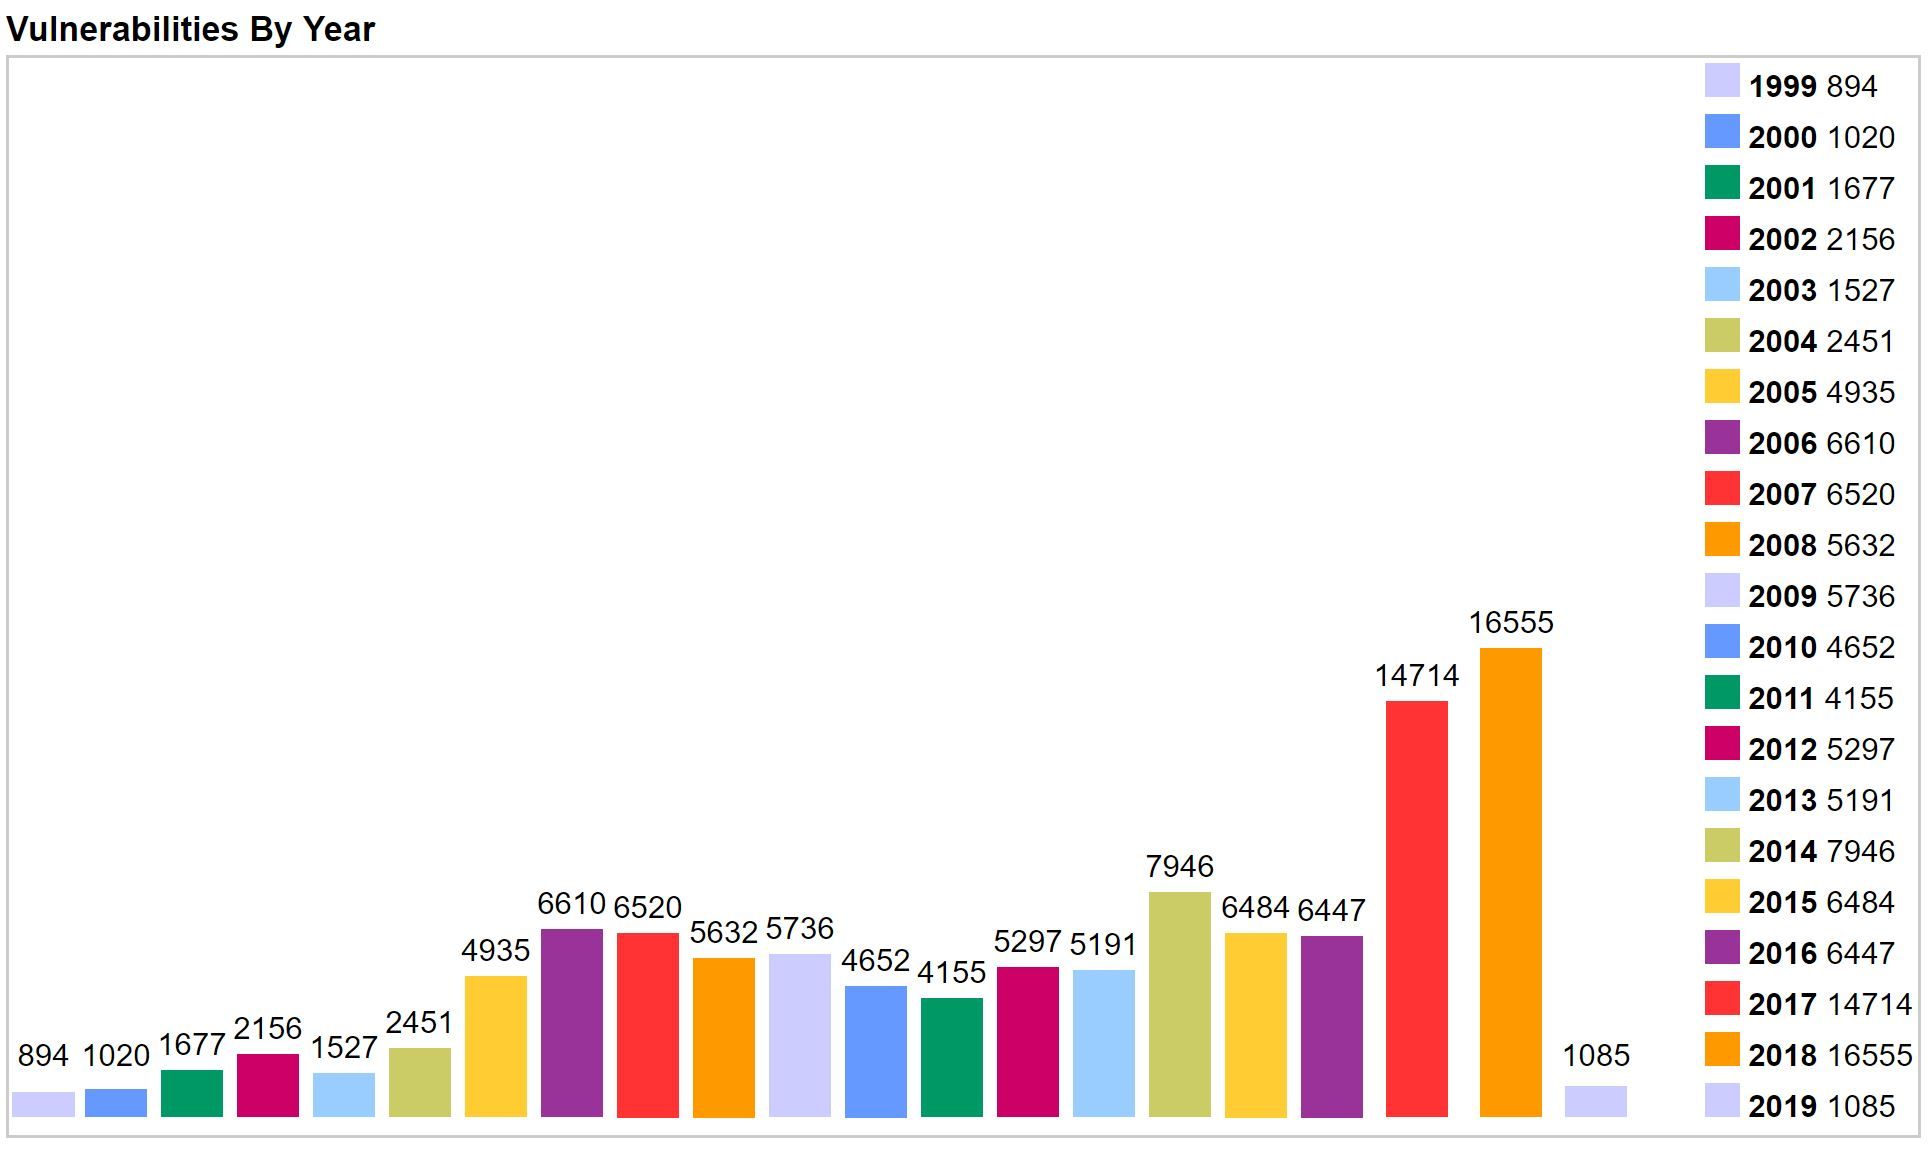
\includegraphics[width=1\textwidth]{Images/VulnByYear}
  \caption[Gefundene Schwachstellen pro Jahr laut CVE Details]{Gefundene Schwachstellen pro Jahr laut CVE Details \cite{cve}}
\end{figure}

Mit der Anzahl der Webanwendungen steigt auch der Einfluss des World Wide Webs auf alle Lebensbereiche, sei es beim Einkaufen im Online-Shop einschließlich diverser Bezahlsysteme, dem Nachrichtenaustausch über Social-Media-Kanäle oder nur zur Informationsgewinnung auf Nachrichtenseiten - die Gesellschaft ist mehr denn je abhängig von der immer größer werdenden Anzahl an verschiedenen Webanwendungen im Internet.
Fortschreitende Digitalisierung und weltweite Vernetzung verursachen jedoch auch immer mehr Sicherheitslücken: laut CVE Details hat sich die Anzahl der gefundenen Schwachstellen in den letzten zwei Jahren mehr als verdoppelt (siehe Abb. 1.1).


Zunehmende Cyberangriffe von kriminellen Hackern aber auch von politisch oder ideologisch motivierten Angreifern sind die Folge. Aktuelle Beispiele sind der Angriff auf die Münchner Firma Krauss Maffai im Dezember 2018, der die Produktion des Maschinen-bauunternehmens für mehrere Tage lahmlegte oder die Attacke auf das Datennetz des Deutschen Bundestags im Oktober 2018. Das Datenleck „Collection \texttt{\#}1“, das im Januar 2019 auftauchte, ist das Ergebnis einer Vielzahl von Cyberattacken, es enthält über 2,6 Milliarden Datensätze mit Zugangsdaten und Passwörtern für hunderte Webseiten.

Für die betroffenen Firmen ist der Schaden enorm: Laut einer Studie des Digitalverbands Bitkom lag der durch Cyberattacken verursachte wirtschaftliche Gesamtschaden für Industrieunternehmen in Deutschland innerhalb der letzten zwei Jahre bei über 43 Milliarden Euro \cite{Bitkom}. Aus der gleichen Studie geht hervor, dass unentdeckte Sicherheitslücken das größte Risiko darstellen (siehe Abb. 1.2)\\

\begin{figure}[htb!]
  \centering
   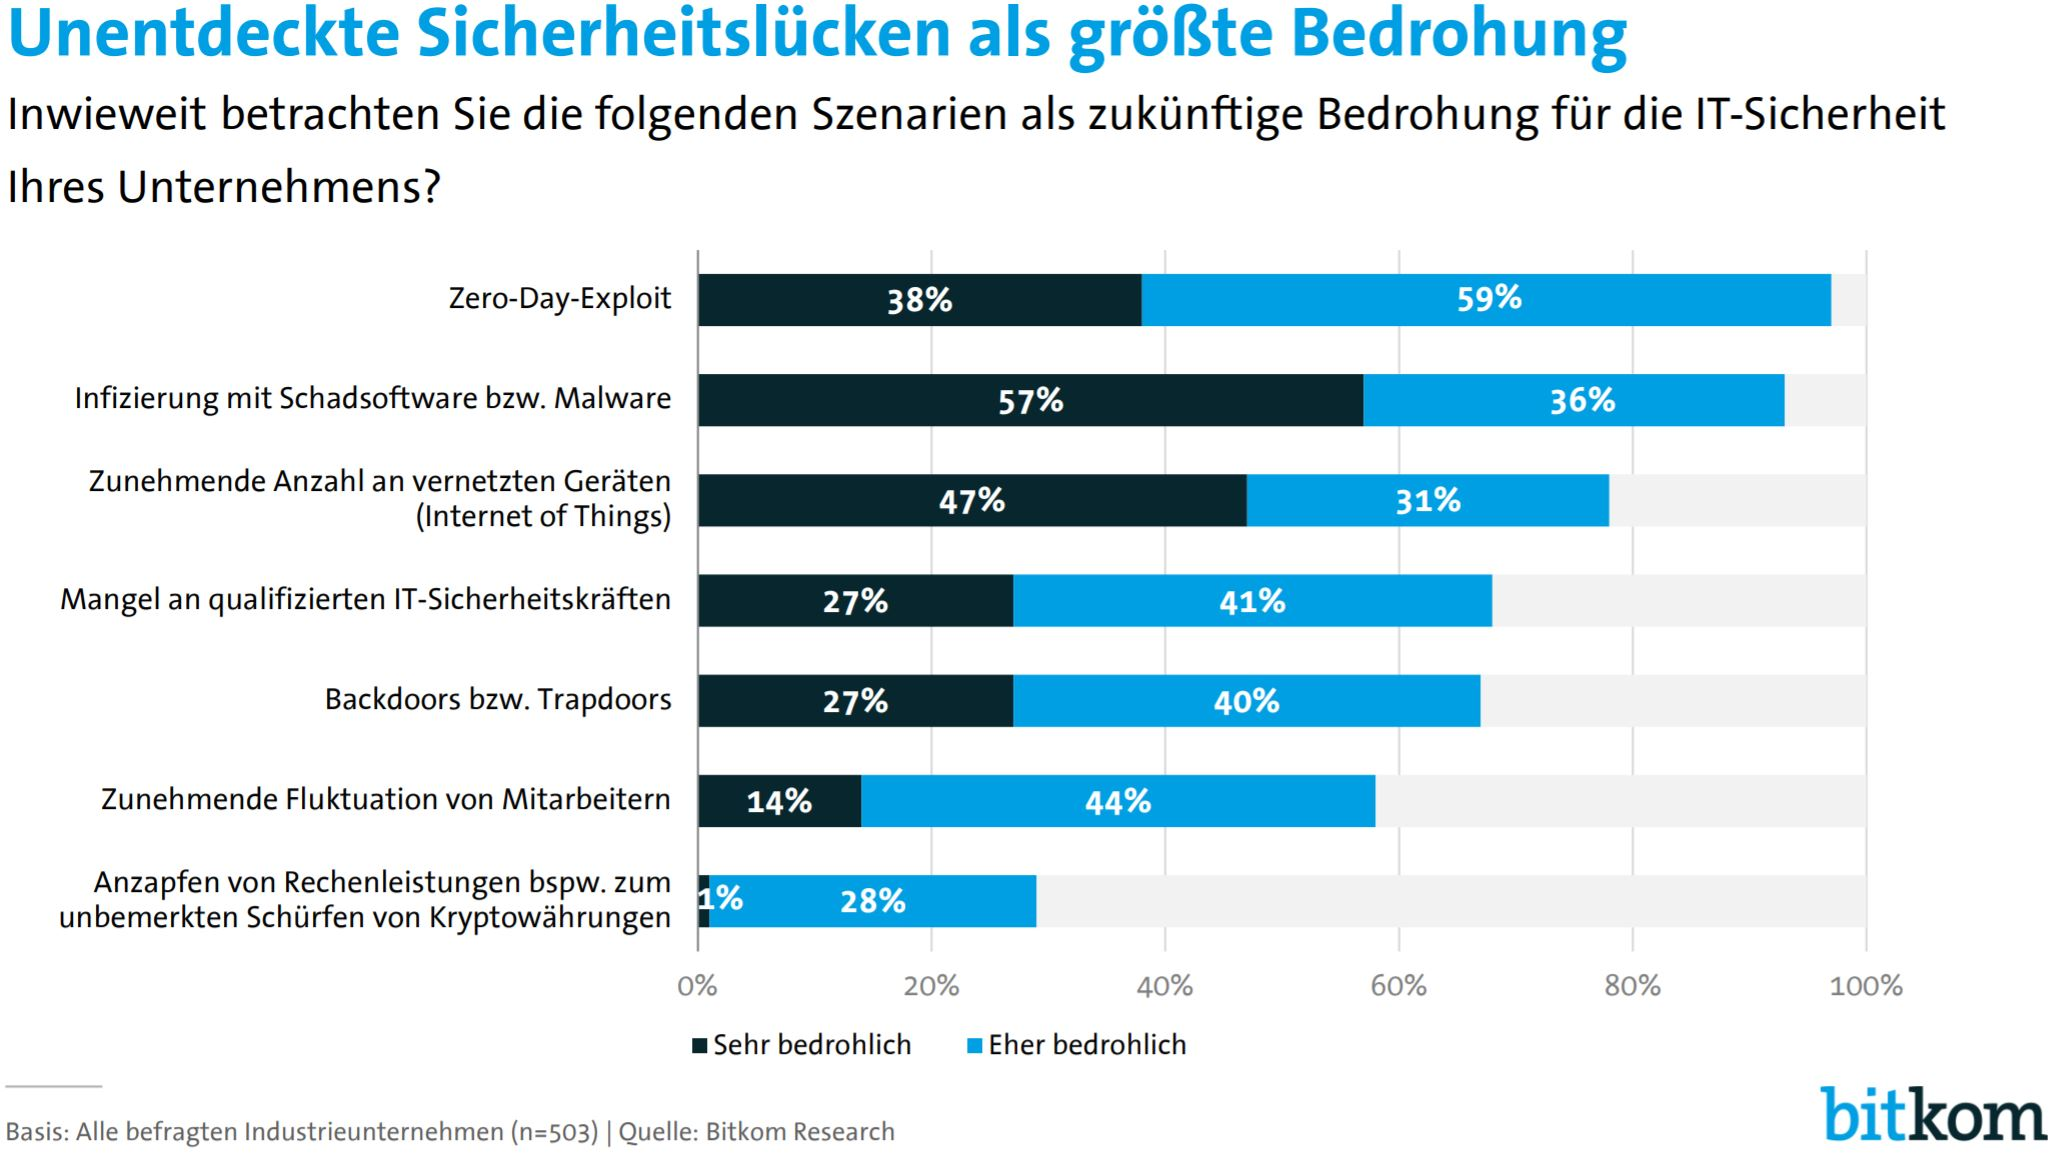
\includegraphics[width=1\textwidth]{Images/Bitkom}
  \caption[Bitkom Studie - Bedrohungsszenarien]{Bitkom Studie - Bedrohungsszenarien \cite{Bitkom}}
\end{figure}
Es gibt mehrere Ansätze, diesem Risiko zu begegnen: Grundsätzlich sollte der Entwickler einer Webseite von Beginn an eine Programmierung anstreben, die bereits bekannte Sicherheitslücken vermeidet und so potentiellen Angreifern möglichst wenig Angriffsfläche bietet. Hier bietet das Bundesamt für Sicherheit in der Informationstechnik (BSI) mit seinem ``Leitfaden zur Entwicklung sicherer Webanwendungen''  \cite{BSI} Hilfestellung.\\
Fehler in der Programmierung lassen sich jedoch nicht immer ausschließen, zudem ist auch ein Schutz gegen unentdeckte Sicherheitslücken vonnöten.

Neben dem Einsatz von Web Application Firewalls ("Web Shields"), die den Datenstrom zwischen Browser und Webapplikation überwachen, ist die Verwendung von Web Application Vulnerability Scannern (WVS) im Rahmen von Penetration Tests ein wesentlicher Bestandteil von Sicherheitskonzepten in diesem Bereich.

WVS überprüfen Webanwendungen automatisiert auf Schwachstellen und unterstützen dadurch den Penetration Tester beim Aufspüren von Sicherheitslücken.

Die vorliegende Arbeit macht sich die Evaluation von WVS zur Aufgabe, da die wenigen bisherigen Ausarbeitungen zu diesem Thema veraltet sind und teilweise andere Ansätze verfolgen:

\begin{itemize}
  \item
  Holm \cite{Holm} vergleicht in seiner Studie aus dem Jahr 2011 lediglich kommerzielle Scanner und verzichtet auf Bewertungskategorien wie Bedienung und Reporting.
  \item
  Wundram \cite{Wundram}\cite{Wundram2} behandelt das Thema zweimal, in seinen Vergleichen von 2011 und 2012 finden sich veraltete Programme wie Watobo oder das inzwischen nicht mehr lauffähige W3af.
\end{itemize}

Zusätzliche Motivation ist die große Anzahl und Vielfalt der Scanner: Das Open Web Application Security Project (OWASP) listet allein eine Sammlung von 50 verschiedenen WVS auf \cite{OWASPtools}, es gibt freie, Open Source und kommerzielle WVS jeweils für verschiedene Plattformen, reine Terminal-Anwendungen und Programme mit grafischer Benutzeroberfläche.
Das Ziel dieser Arbeit ist es, aus dieser bunten Mischung diejenigen WVS herauszufiltern, für die eine nähere Betrachtung lohnenswert erscheint und diese im Hinblick auf folgende Fragestellungen zu evaluieren:

\textbf{1. Wieviele Schwachstellen werden von den WVS gefunden?}

\textbf{2. Wie unterscheiden sich die WVS in den Kategorien Bedienung, Reporting und Scan-Geschwindigkeit?}

\textbf{3. Welcher WVS schneidet insgesamt am besten ab?}
\newpage

\textbf{4. Wie schneiden die Open Source WVS im Vergleich mit kommerziellen WVS ab?}

Die Evaluation soll mit Hilfe eines Punktesystems erfolgen und schließlich in einem Ranking resultieren, das die Tauglichkeit und Qualität der getesteten WVS anhand ihrer Platzierungen aufzeigt.

Die Arbeit ist in sechs Kapitel aufgeteilt:

\textbf{1. Einführung:} In der Einführung wird der Leser an das Thema herangeführt, die Motivation und die Zielsetzung  sowie die zentralen Fragestellungen und der Aufbau der Arbeit werden erläutert.

\textbf{2. Grundlagen:} Das zweite Kapitel vermittelt Grundlagen über Webanwendungen, Schwachstellen,  Sicherheitsmaßnahmen wie Web Application Firewalls und Penetrationtesting sowie die Arbeistweise von WVS.

\textbf{3. Methodik:} Hier wird der Testaufbau beschrieben einschließlich der Auswahlkriterien für die WVS und des Punktesystems für die Bewertung. Nicht berücksichtigte WVS werden beschrieben sowie die verwundbaren Webanwendungen, die für die Tests verwendet wurden.

\textbf{4. Evaluation:} Dieses Kapitel beinhaltet die Ergebnisse der Evaluation, zum einen die Anzahl der gefundenen Schwachstellen per WVS, zum anderen eine Beschreibung der WVS einschließlich der Bewertung in den Kategorien Bedienung, Reporting und Scangeschwindigkeit.



\textbf{5. Diskussion:} In diesem Kapitel werden die Ergebnisse der Evaluation durchleuchtet und erörtert.


\textbf{6. Fazit und Ausblick:} Zum Schluss wird die Studie nochmals zusammengefasst und auf mögliche zukünftige Arbeiten verwiesen.\\

Dieser Arbeit wurde eine CD-ROM beigelegt, die sämtliche Berichte aller durchgführten Scans enthält.

\chapter{Grundlagen}
  \section{Webanwendung}
  Zu Beginn sollte der Begriff ``Webanwendung'' geklärt werden.
  Eine Webanwendung muss nicht zwingend über das World Wide Web erreichbar sein, auch in vielen Unternehmen kommen Webanwendungen zum Einsatz. Ob eine Anwendung als Webanwendung bezeichnet werden kann, hängt vom Einsatz von Webtechnologien ab. Daraus kann folgende Begriffsdefinition abgeleitet werden \cite[S.1]{Rohr}:

  \begin{quote}``Eine Webanwendung ist eine Client-Server-Anwendung, die auf Webtechnologien (HTTP, HTML etc.) basiert.''\end{quote}

  Eine Webanwendung wird über einen Browser aufgerufen, der den serverseitig bereitgestellten HTML-, Java-Script oder CSS-Code interpretiert und darstellt. Danben kann auch über ein Skript oder von einer Kommandozeile aus auf Webanwendungen zugegriffen werden, man spricht hier von einem User Agent oder Client.
  Zur Kommunikation zwischen Browser (also Client) und Server wird das HTTP-Protokoll verwendet oder das darauf aufsetzende HTTPS-Protokoll.
  Serverseitig werden Webanwendungen auf Web- und Applikationsservern oder Laufzeitumgebungen ausgeführt, die dann wiederum auf Hintergrundsysteme wie Datenbanken zugreifen können.

  Daraus ergibt sich eine sogenannte 3-Tier-Architektur (dreischichtige Architektur, siehe Abb. 2.1).
  \begin{figure}[H]
    \centering
     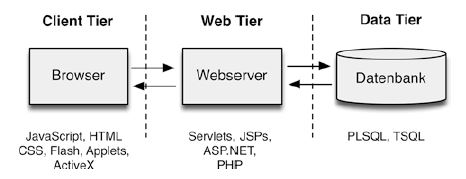
\includegraphics[width=0.7\textwidth]{Images/3_Tier_Architektur}
    \caption[3-Tier-Architektur einer Webanwendung]{3-Tier-Architektur einer Webanwendung \cite{Rohr}}
  \end{figure}

  Moderne Webanwendungen lassen sich jedoch - insbesondere im Enterprise-Umfeld - nicht als einzelne Anwendungen sehen, sondern als Zusammenschluss verschiedener eigenständiger Dienste wie REST- oder Microservices zu einer Plattform, wie z.B. einem Onlineshop (siehe Abb. 2.2).
  \begin{figure}[H]
    \centering
     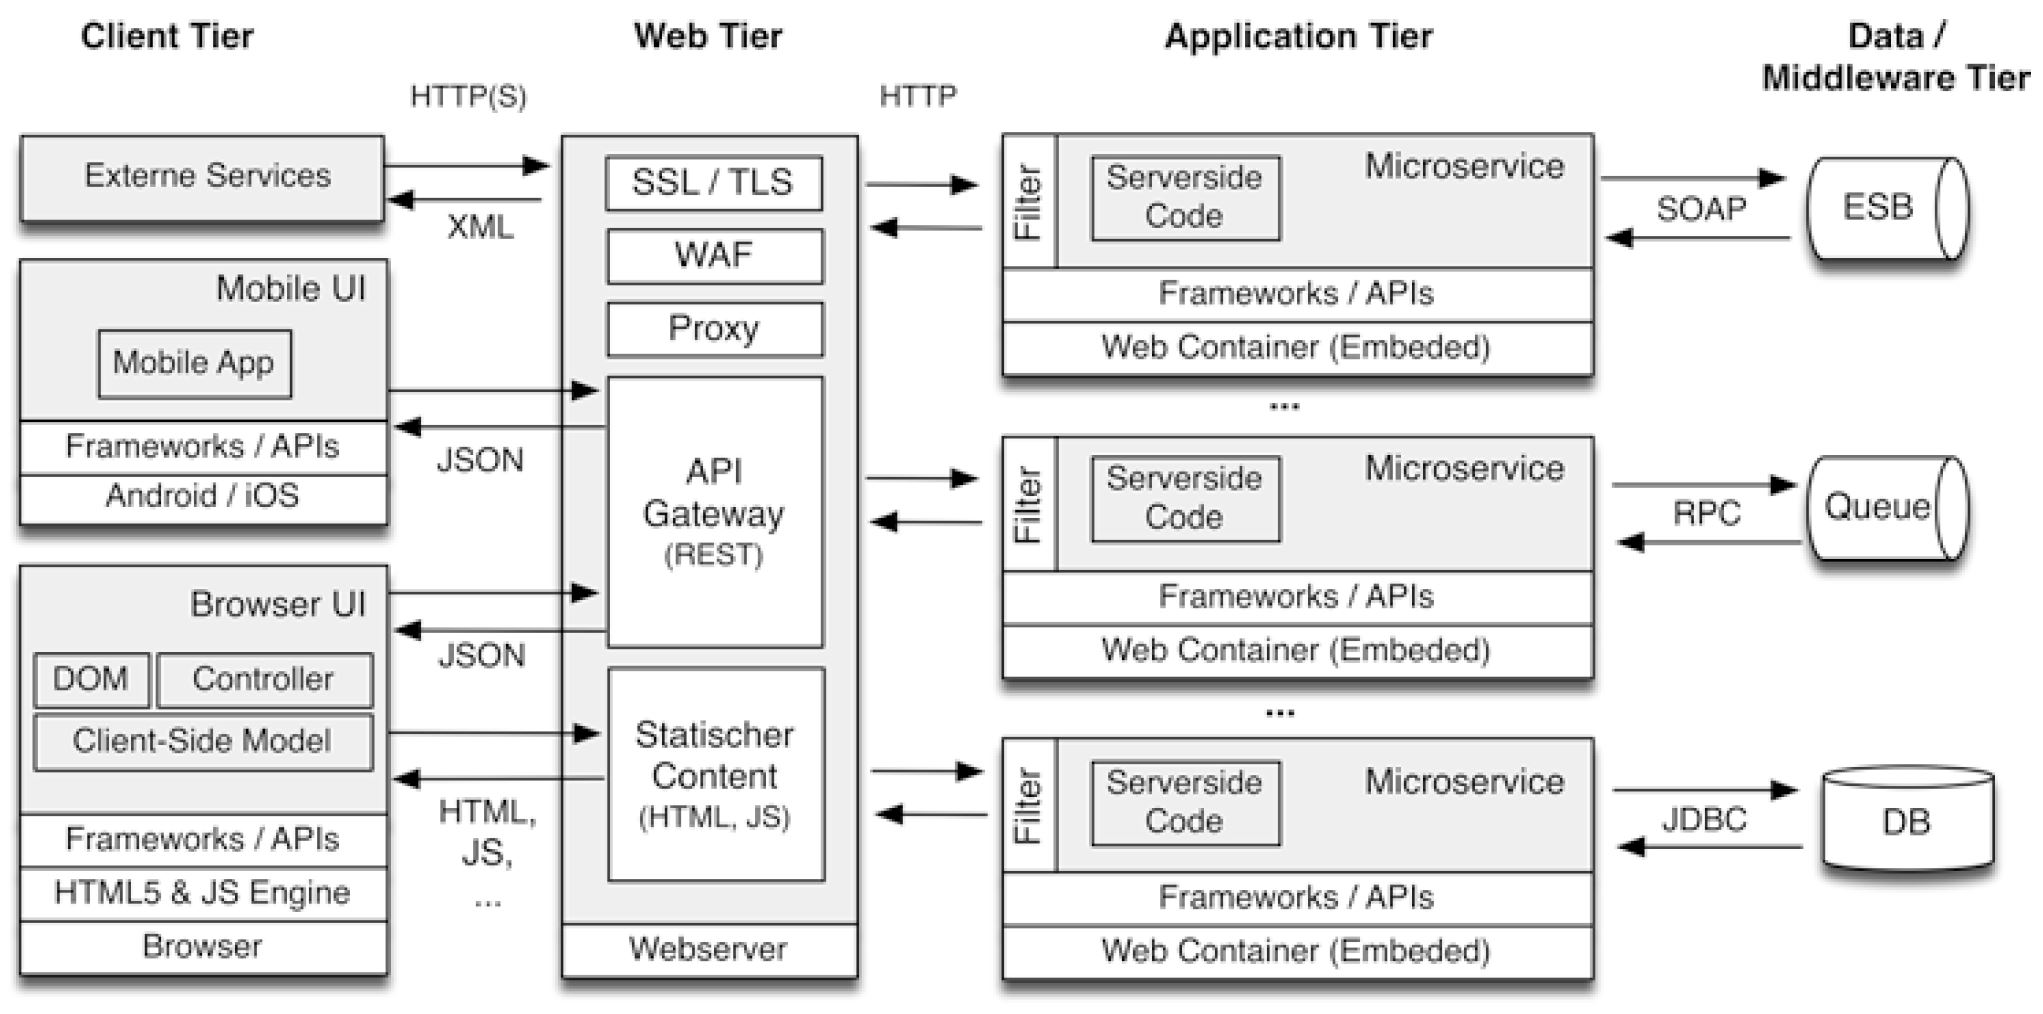
\includegraphics[width=1\textwidth]{Images/Enterprise}
    \caption[Enterprise Webanwendung auf Basis einer Microservice-Architektur]{Enterprise Webanwendung auf Basis einer Microservice-Architektur \cite{Rohr}}
  \end{figure}

  Im Zuge der Weiterentwicklung von Webanwendungen werden immer mehr Aspekte der Benutzerschnittstelle client-seitig, vor allem über JavaScript-Code umgesetzt, der im Hintergrund serverseitige Webdienste aufruft.
  Diese Verlagerung von Anwendungslogik vom Server auf den Client resultieren in sogenannten Single Page Applications (SPAs), die nur noch aus einer einzigen HTML-Seite mit sehr viel JavaScript-Code bestehen, der im Hintergrund auf der Serverseite mit REST-Services kommuniziert und die Anzeige der Seiteninhalte steuert. Ein bekanntes Beispiel für solch eine Single Page Application ist Google Mail.
  \cite{Rohr}
  \newpage

 \section{Schwachstellen}
  Das BSI definiert eine Schwachstelle wie folgt:

  \begin{quote}``Eine Schwachstelle (englisch ``vulnerability'') ist ein sicherheitsrelevanter Fehler eines IT-Systems oder einer Institution. Ursachen können in der Konzeption, den verwendeten Algorithmen, der Implementation, der Konfiguration, dem Betrieb sowie der Organisation liegen. Eine Schwachstelle kann dazu führen, dass eine Bedrohung wirksam wird und eine Institution oder ein System geschädigt wird. Durch eine Schwachstelle wird ein Objekt (eine Institution oder ein System) anfällig für Bedrohungen.'' \cite[S.107]{BSI2}
  \end{quote}

  Im Idealfall entdeckt ein Hersteller Schwachstellen selbst und kann sie beheben, bevor sie öffentlich bekannt werden. Sollte die Sicherheitslücke jedoch durch Dritte gefunden werden, kann ihr Lebenszyklus und die Gefährdung für die Nutzer unterschiedlich verlaufen. Der Verlauf hängt in erster Linie vom Entdecker, aber auch von der Reaktion der Hersteller ab \cite{BSI3}:
  \begin{itemize}
    \item Möchte der Entdecker die IT-Sicherheit verbessern, oder hat er kriminelle Absichten und benutzt die Schwachstelle für eigene Interessen?
    \item Inwieweit wird die Öffentlichkeit über die Schwachstelle informiert?
    \item Ist der Hersteller in der Lage, die Sicherheitslücke schnell zu beheben?
  \end{itemize}
Um bekannte Schwachstellen herstellerübergreifend einheitlich benennen zu können, wurde der Industriestandard Common Vulnerabilities and Exposures (CVE) etabliert, der gewährleistet, dass Hersteller, Entdecker und weitere Beteiligte jeweils über dieselbe Schwachstelle diskutieren. Der CVE sammelt vorhandene Informationen über die Schwachstelle und bietet die Möglichkeit zu statistischen Auswertungen.

  Wie in Abbildung 2.3 dargestellt, lässt sich der Lebenszyklus einer Schwachstelle, die durch Dritte entdeckt wurde, auf das folgende Schema zurückführen\cite{BSI3}:

  1. Entdeckung der Schwachstelle durch einen Dritten.

  2. Es gibt mehrere Möglichkeiten, wie der Hersteller von der Schwachstelle erfährt:
  \begin{itemize}
    \item \glqq Full Disclosure\grqq: Alle Informationen über die Schwachstelle werden vom Entdecker öffentlich gemacht.
    \item \glqq Coordinated Disclosure\grqq: Der Entdecker kontaktiert direkt den Hersteller und koordiniert mit ihm das weitere Vorgehen, hier werden zunächst keine Informationen an die Öffentlichkeit gegeben.
    \item \glqq Zero-Day-Exploit\grqq: Niemand wird über die Schwachstelle informiert, stattdessen wird sie für Angriffe ausgenutzt. Öffentlichkeit und Hersteller erfahren erst nach erfolgreichen Angriffen von der Schwachstelle.
    \item Indirekte Benachrichtigung an den Hersteller über einen sogenannten Schwachstellen-Broker. \end{itemize}
  3. Der Hersteller beginnt damit, die Sicherheitslücke zu schließen, indem er die Software nachbessert und einen Patch entwickelt.

  4. Veröffentlichung eines ``Advisorys'', einer Schwachstellenwarnung, die Informationen über die Sicherheitslücke, eine Gefährdungsbewertung und vorläufige Gegenmaßnahmen beinhaltet.
  Das Advisory erscheint in der Regel zeitgleich mit dem Patch, bei hoher Gefährdung und wenn die Öffentlichkeit schon von der Schwachstelle erfahren hat, kann es auch vor der Fertigstellung des Patches veröffentlicht werden.

  5. Der Patch ist fertiggestellt und wird vom Hersteller mit einer entsprechenden Beschreibung (Bulletin) zur Verfügung gestellt. Mit der Veröffentlichung des Patches und dem Bulletin steigt die Gefahr für ungepatchte Systeme, da nun auch potentelle Angreifer umfangreiche Informationen über die Schwachstelle
  erhalten.

  6. Der Patch wird von den Benutzern der betroffenen Software installiert und die Sicherheitslücke dadurch geschlossen.

  Der Ablauf kann von diesem Schema abweichen; wenn beispielsweise eine Schwachstelle vom Hersteller zunächst als nicht kritisch eingestuft und daher auf die Entwicklung eines Patches verzichtet wird, kann dies dazu führen, dass zu einem späteren Zeitpunkt schnell reagiert werden muss, wenn sich die Schwachstelle doch als ausnutzbar erweist. \cite{BSI3}

  \begin{figure}[H]
    \centering
     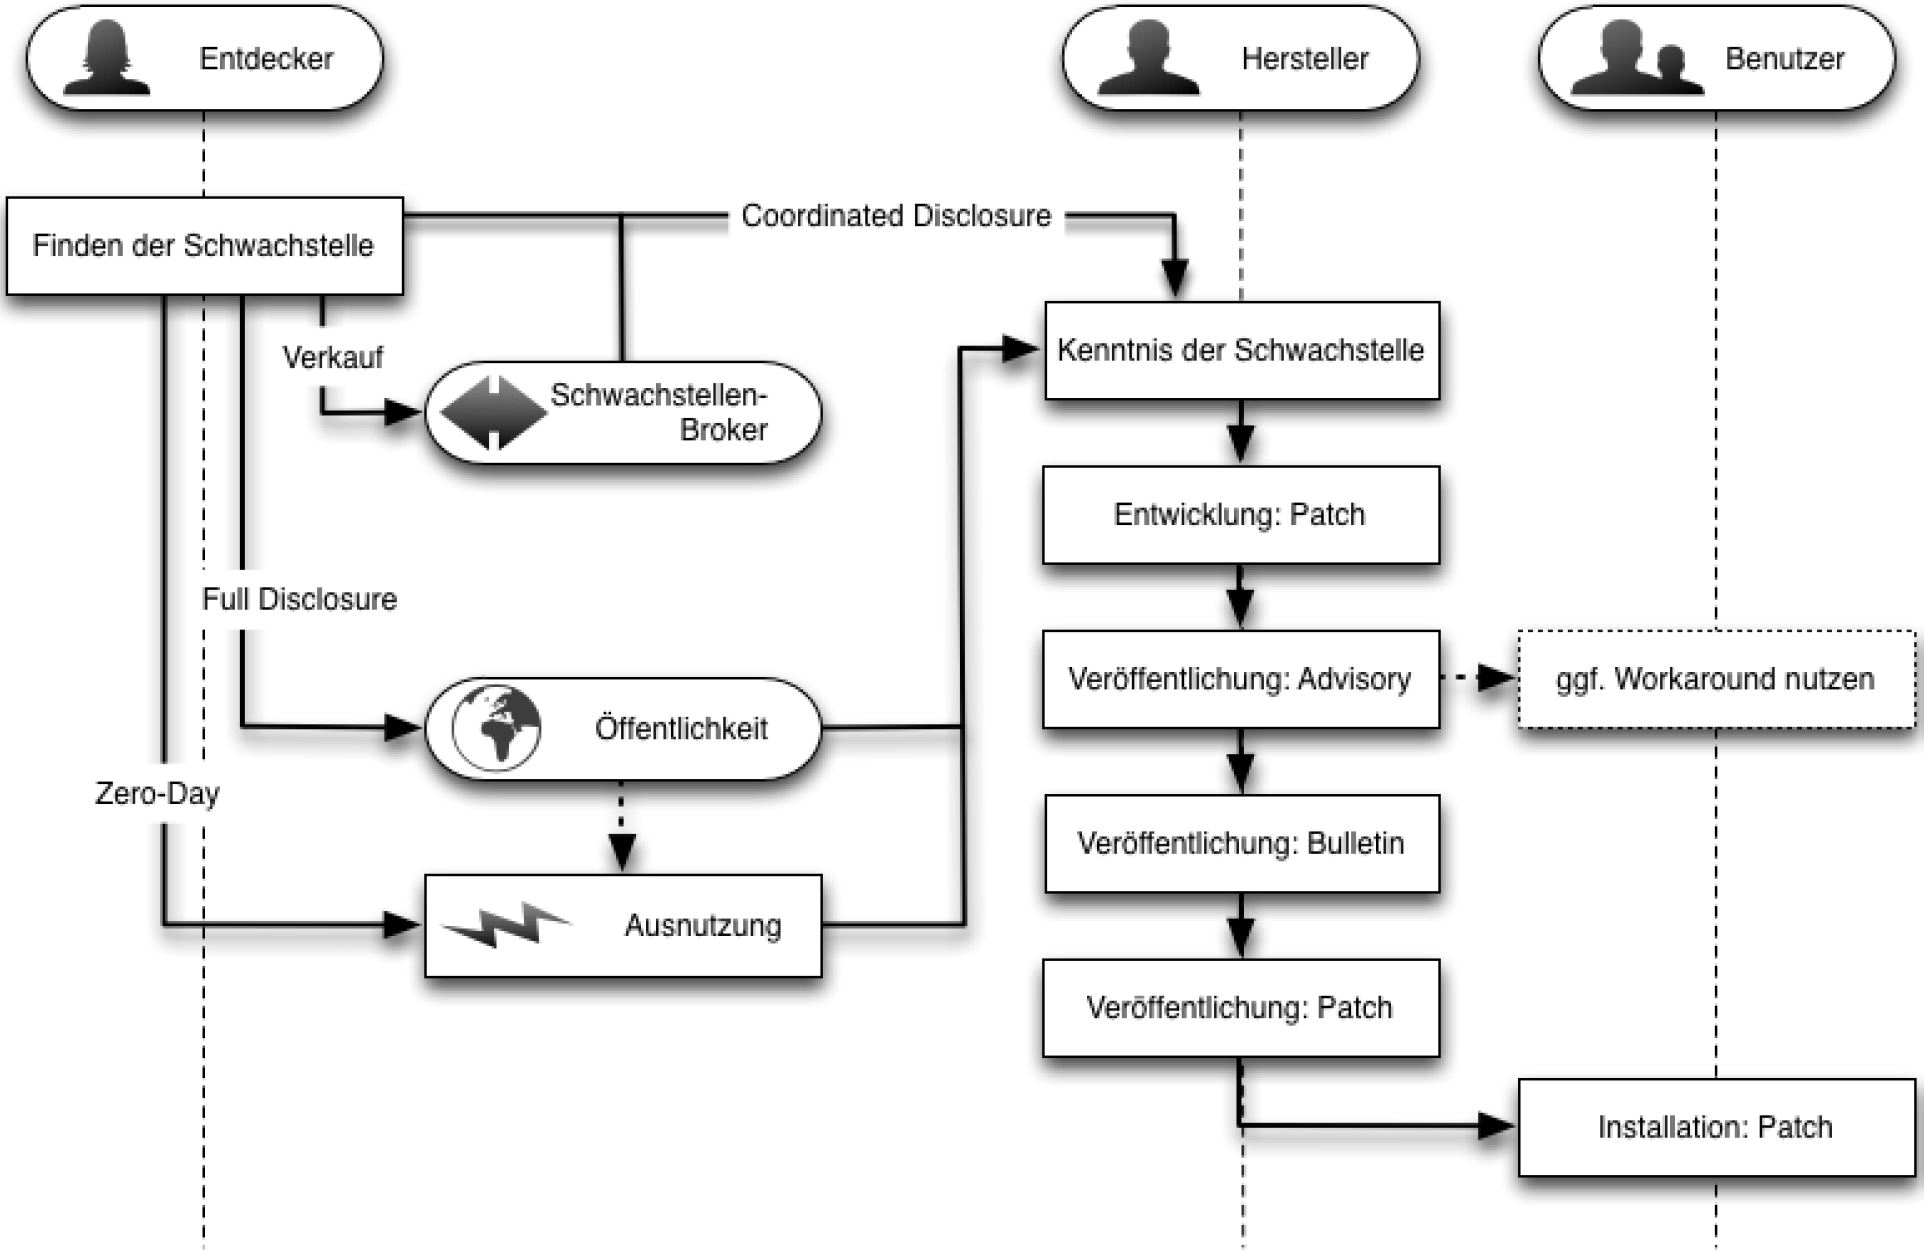
\includegraphics[width=1\textwidth]{Images/Lebenszyklus}
    \caption[Lebenszyklus einer Schwachstelle]{Lebenszyklus einer Schwachstelle \cite{BSI3}}
  \end{figure}



  \section{Web Application Security}
  Die Webanwendungssicherheit ist ein Teilgebiet der IT-Sicherheit und befasst sich vor allem mit dem Schutz von Assets einer Webanwendung. Als Assets werden Bestandteile einer Webanwendung wie Daten, Systeme oder Funktionen bezeichnet, die Schutzbedarf im Hinblick auf die primären Schutzziele haben \cite{BSI}.

  Diese primären Schutzziele lauten \cite{BSI}:
    \begin{itemize}
    \item Vertraulichkeit
    \item Integrität
    \item Verfügbarkeit
  \end{itemize}

  Aus diesen primären Schutzzielen lassen sich auch sekundäre Schutzziele wie z.B. Authentizität oder Nicht-Abstreitbarkeit ableiten.

  Das Thema Webanwendungssicherheit bezieht sich auf den gesamten Lebenszyklus einer Webanwendung und ist ein wichtiger Bestandteil der Qualitätssicherung. Neben der Bedrohungsabwehr und der Vorbeugung von Sicherheitslücken befasst sie sich auch mit deren Identifizierung und Behebung. \cite{BSI}

  \subsection{Bedrohungen und Risiken}
  Die schwerwiegendsten Angriffe auf Webanwendungen sind sicherlich diejenigen, die sensible Daten verfügbar machen oder uneingeschränkten Zugriff auf die Systeme ermög- lichen, auf denen die Anwendung ausgeführt wird. Hierzu gehören Angriffe per XSS oder SQL-Injection. Aber auch Angriffe, die Systemausfälle versursachen (Denial-of-Service Attacken) stellen für viele Unternehmen ein sehr kritisches Ereignis dar.\\
  Mehrere Organisationen haben es sich zur Aufgabe gemacht, Sicherheitsrisiken für Webanwendungen zu katalogisieren und zu klassifizieren. Das Web Application Security Consortium (WASC), ein Zusammenschluss von Sicherheitsexperten, die an Sicherheitsstandards für Webanwendungen arbeiten, hat mit seiner ``WASC Threat Classification v.2.0'' einen umfassenden Katalog mit Bedrohungen herausgegeben \cite{WASC}.\\
  OWASP veröffentlicht alle drei bis vier Jahre mit den ``OWASP Top Ten'' \cite{OWASPtop10} eine Liste mit den 10 häufigsten Sicherheitsrisiken für Webanwendungen, die durch die große Akzeptanz in der Fachwelt als Sicherheitsrichtlinie angesehen werden kann.


  \subsection{Sicherheitsmaßnahmen}
  Das BSI definiert den Begriff wie folgt:
    \begin{quote} ``Als Sicherheitsmaßnahmen werden alle Aktionen bezeichnet, die dazu dienen, Sicherheitsrisiken zu steuern und diesen entgegenzuwirken. Dies schließt sowohl organisatorische, als auch personelle, technische oder infrastrukturelle Sicherheitsmaßnahmen ein. Synonym werden auch die Begriffe Sicherheitsvorkehrung oder Schutzmaßnahme benutzt.'' \cite[S.107-108]{BSI2}\end{quote}

 Zu den Maßnahmen, die bereits während der Entwicklung ergriffen werden sollten, gehören umfangreiche Security Tests. Nach Inbetriebnahme der Webanwendung kann mit Hilfe von Penetration Tests nach Sicherheitslücken gesucht werden, zusätzlichen Schutz bieten Web Application Firewalls.


  \subsubsection{Security Tests}

  Bevor eine Webanwendung ausgeliefert wird, sollte sie mit Hilfe von Security Assessments  auf Sicherheitsmängel getestet werden.
  Ein Security Assessment soll dabei sicherstellen, dass die definierten Sicherheitsanforderungen in der
  Implementierungsphase korrekt umgesetzt worden sind. Zusätzlich soll in diesem Rahmen auch die
  Effektivität der gesetzten Sicherheitsanforderungen überprüft werden und so mögliche Unzulänglichkeiten
  in der Spezifikation selbst aufgedeckt werden. Das heißt, es soll sichergestellt werden, dass die spezifizierten Sicherheitsanforderungen auch angemessen und wirksam sind.
  Üblicherweise durchlaufen Security Assessments die folgenden Phasen \cite{BSI}:
  \begin{itemize}
    \item Planung: Ein Security Assessment benötigt eine initiale Planung. Hier werden sämtliche
    Informationen, die für die Durchführung des Assessments notwendig sind, zusammengetragen.
    \item Durchführung: Die Hauptaufgabe dieser Phase ist das Suchen nach Schwachstellen und deren
    Bewertung.
    \item Auswertung: Hierbei werden die gefundenen Schwachstellen analysiert. Es werden die Ursachen
    und die Gegenmaßnahmen bestimmt und in einem Abschlussbericht zusammengefasst. Der
    Abschlussbericht wird an die Entwickler geleitet, die die identifizierten Schwachstellen beheben.
    Nach der Behebung werden die Schwachstellen erneut untersucht.
  \end{itemize}
  Die Überprüfung kann unter Verwendung mehrerer verschiedener Testverfahren erfolgen. Dabei ist zu
  berücksichtigen, dass unterschiedliche Testverfahren unterschiedliche Aufgaben erfüllen und
  unterschiedliche Ergebnisse liefern. Beispielsweise überprüfen Unit Tests die Korrektheit und die
  vollständige Abdeckung einer Funktionalität, während ein Code Review die korrekte Implementierung
  überprüft. Je nachdem was genau überprüft werden soll, können auch unterschiedliche Testrollen
  herangezogen werden. Ein Auditor kann beispielsweise die Einhaltung von Vorgaben überprüfen, während
  ein Penetrationstester die korrekte Implementierung überprüft.

  Folgende Testverfahren können bereits während der Implementierung durchgeführt werden \cite{BSI}:
  \begin{itemize}
    \item Security Test Cases:
    Ein Test Case beschreibt einen Softwaretest, in dem die laut den Sicherheitsanforderungen
    bestimmte spezifizierte Funktionalität (funktional oder nicht funktional) der Webanwendung auf
    ihre Korrektheit überprüft wird. Test Cases einer Webanwendung werden hierbei in einfacher
    Sprache beschrieben.
    Ein Test Case besteht immer zumindest aus einer eindeutigen ID, einer Beschreibung und einem
    erwarteten Ergebnis.
    Im Zuge des Tests Cases muss die Einhaltung des erwarteten Ergebnisses überprüft werden.
    Test Cases lassen sich in folgende Arten unterteilen:

    - Positivtest: Das Verhalten der Webanwendung wird mit gültigen Rahmenbedingungen und
    Eingaben überprüft.

    - Negativtest: Das Verhalten der Webanwendung wird mit ungültigen Rahmenbedingungen
    und Eingaben überprüft.

    Test Cases sollten priorisiert werden. Jedem Test Case wird ein je nach Kritikalität der zugehörigen
    Funktion ein Prioritätslevel (z.B. Normal, Hoch, Kritisch) zugewiesen und beim Testen
    berücksichtigt.
    Test Cases müssen im Rahmen der Entwicklung durch den Entwickler erstellt werden.
    \item Security Unit Tests:
    Unit Tests überprüfen Softwareeinheiten (Units) einer Webanwendung auf korrekte Funktionalität.
    In der Regel sind das Funktionen, Methoden oder Klassen. Units werden mit verschiedenen
    Parametern aufgerufen und es wird überprüft, ob die Ausgabe mit den Erwartungen
    übereinstimmt.
    Unit Tests müssen im Rahmen der Entwicklung durch die Entwickler erstellt und gepflegt werden.
    \item Design Review:
    Bei Design Reviews geht es darum, die Architektur der Anwendung auf hoher Ebene zu
    untersuchen. Dabei sollen konzeptionelle Fehler und Verwundbarkeiten aufgedeckt werden und
    die Umsetzung der Sicherheitsanforderungen und -mechanismen auf ihre Vollständigkeit hin
    untersucht werden. Wenn erhebliche Mängel im Design erkannt werden, muss die Konzeption und die Planung überarbeitet werden. Die im Design Review erkannten Mängel dienen hierbei als Ansatzpunkt.
    \item Code Reviews:
    Beim Code Review wird der Programmcode manuell überprüft. Hierbei ist zu beachten, dass die
    Durchsicht durch eine andere Person erfolgt (etwa innerhalb eines Peer Reviews) als derjenigen, die
    den Programmcode verfasst hat, da ansonsten Fehler leicht übersehen werden können. Typische
    Fehler, die entdeckt werden können, sind Abweichungen von Standards, Abweichungen gegenüber
    Anforderungen, Fehler im Design, Buffer Overflows etc. In erster Linie ist das bei sensitiven
    Funktionen wie beispielsweise Transaktionsmanagement, Authentisierung und Kryptographie
    wichtig. Die Ergebnisse des Code Reviews fließen zurück in den Implementierungsprozess.
    \item Statische Code Scanner:
    Mittels Statischer Code Analyse (SCA) können eine Vielzahl von Schwachstellen bereits innerhalb
    der Entwicklung identifiziert und so zeitnah behandelt werden. In der Praxis ist die Auswahl
    entsprechender Tools zur Durchführung von Sicherheitsscans sehr beschränkt. Weiterhin müssen
    diese Tools die eingesetzten Technologien unterstützen. Analysieren sie den Sourcecode, müssen
    diese zusätzlich die eingesetzten APIs kennen, da diese gewöhnlich nicht im Sourcecode vorliegen.
    Schließlich erzeugen SCA-Tools häufig eine sehr hohe Anzahl an False Positives, weshalb eine
    Verifikation der Scanergebnisse durch fachmännisches Personal erforderlich ist.
    \item Web Application Vulnerability Scanner: siehe 2.3
    \item Fuzz Testing:
    Fuzz Testing ist ein Testverfahren, welches automatisiert oder teilweise automatisiert durchgeführt
    wird. Dabei werden ungültige, unerwartete oder zufällige Werte generiert und als Eingabe an die
    Anwendung weitergegeben. Das Verhalten der Anwendung wird während des Tests auf
    Fehlverhalten überwacht. Das Prinzip ist simpel und führt dazu, dass Fehler entdeckt werden, die
    oft übersehen worden wären. Fuzz Testing kann nur einfache Programmfehler entdecken, die auf
    falsche Eingabewerte zurückzuführen sind, jedoch keine Designfehler etc. \cite{BSI}
  \end{itemize}

    \subsubsection{Penetration Testing}
    Nach Fertigstellung der Webanwendung kommen Penetration Tests zum Einsatz. Sie können als legaler und autorisierter Versuch definiert werden, Computersysteme anzugreifen, mit dem Ziel, diese sicherer zu machen.
    Der Prozess umfasst die Suche nach Schwachstellen sowie die Demonstration von Beispielangriffen, um zu zeigen, dass die Bedrohungen real sind.
    Ein ordnungsgemäßer Penetration Test resultiert immer in spezifischen Empfehlungen für das
    Beheben der während des Tests aufgetretenen Probleme.
    Insgesamt wird dieses Verfahren dazu verwendet, Computer und Netzwerke gegen zukünftige Angriffe abzusichern. Die allgemeine Idee besteht darin, Sicherheitslücken mithilfe der gleichen Tools und Techniken zu finden, die auch ein Angreifer benutzt. Die Lücken können so geschlossen werden, bevor ein realer Hacker sie ausnutzt. \cite{engebretson}

    Üblicherweise lassen sich Penetration Tests in mehrere Phasen unterteilen \cite{BSI}:

    \begin{itemize}
      \item Informationsgewinnung
      \item Identifizierung der Angriffsfläche
      \item Identifizierung von System und Anwendungen
      \item Schwachstellenrecherche und Priorisierung der Schwachstellen nach Ausnutzbarkeit und Auswirkung
      \item Angreifen der Schwachstellen
    \end{itemize}

    Penetration Tests können basierend auf unterschiedlichen Kriterien klassifiziert werden \cite{BSI}:
    \begin{itemize}
      \item Informationsbasis: Hier wird festgelegt, von welchem Wissensstand der Tester ausgeht.
      \item Aggressivität: Hier wird festgelegt, wie aggressiv der Angreifer vorgeht. z.B. passiv (gefundene
      Schwachstellen werden nicht ausgenutzt) oder aggressiv (gefundene Schwachstellen werden
      unabhängig von den Konsequenzen ausgenutzt).
      \item Umfang: Hier wird festgelegt, welche Systeme getestet werden.
      \item Vorgehensweise: Der Angreifer kann verdeckt (Penetration wird nicht direkt als Angriff erkannt)
      oder offensichtlich (Penetration erfolgt offensichtlich) vorgehen.
      \item Technik: Es muss definiert werden, welche Techniken eingesetzt werden. Erfolgt der Angriff z.B. nur
      über das Netzwerk oder auch über weitere Kommunikationsnetze (Telefon, physischer Zugriff etc.)?
      \item Ausgangspunkt: Hier wird festgelegt, ob der Penetration Test von innen oder von außen erfolgen
      soll. Man unterscheidet hier zwischen drei unterschiedlichen Ansätzen, dem Black-Box, Grey-Box und White- Box Testing:

    Beim Black-Box Testing befindet sich der Tester in der Rolle eines typischen Hackers von
    außen, der kein Wissen über die innere Arbeitsweise der Anwendung hat, weder Architektur noch
    Quellcode sind bekannt. Der Angreifer muss mit manuellen Methoden sowie speziellen Tools des Penetration Testings vertraut sein, um Schwachstellen zu lokalisieren und auszunutzen. Für die dynamische Analyse des anzugreifenden Netzwerks benötigt er Scanning Tools, die in der vorliegenden Arbeit evaluiert werden.

    Während der Black-Box-Tester ein System aus der Sicht eines Außenseiters untersucht, hat ein    Grey-Box Tester bereits Zugriff auf das System auf Benutzerebene, möglicherweise sogar mit erhöhten Berechtigungen eines Administrators. In der Regel liegt eine Dokumentation über Design und Architektur des Netzwerks vor, die internen Komponenten sind bekannt. Dies hat den Vorteil, dass die Sicherheit des Netzwerks gezielter und effizienter beurteilt werden kann, der Tester kann sich sofort auf die Systeme konzentrieren, die am wichtigsten sind oder ein besonders hohes Risiko haben. Zudem kann durch das interne Benutzerkonto ein Angriff innerhalb des abgesicherten Systems mit umfassendem Zugriff auf das Netzwerk simuliert werden.

    Der White-Box Tester hat schließlich uneingeschränkten Zugriff auf ein System, er besitzt alle nötigen Berechtigungen und kennt Netzwerkarchitektur und Design. Überdies hat er Zugang zum Quellcode, was es ihm erlaubt, statische Code-Analysen durchzuführen. Durch das Auffinden sowohl interner als auch externer Schwachstellen ist das White-Box Testing maximal effektiv, aber auch sehr aufwandsintensiv da der Tester sehr große Datenmengen untersuchen muss.
    \end{itemize}

    Penetration Tests können nicht nur auf technische Systeme, sondern auch auf die organisatorische oder
    personelle Infrastruktur in Form von Social Engineering erfolgen.
    Unabhängig von der Vorgehensweise haben Penetration Tests folgende Ziele \cite{BSI}:
    \begin{itemize}
      \item Erhöhung der Sicherheit der IT-Systeme
      \item Identifikation von Schwachstellen
      \item Bestätigung der Sicherheit der IT-Systeme von unabhängigen Dritten
      \item Erhöhung der Sicherheit der organisatorischen und personellen Infrastruktur
    \end{itemize}

    In jedem Fall liefern Penetration Tests die Sicherheitslücken zwischen Planung und Implementierung. Die
    getroffenen Maßnahmen, um die Lücken zu schließen, müssen in einem weiteren Schritt nicht nur auf ihre
    korrekte Umsetzung überprüft werden, sondern auf ihre Angemessenheit, wie effektiv sie das Risiko
    tatsächlich senken beziehungsweise beseitigen oder ob durch sie ein falsches Sicherheitsgefühl vermittelt
    wird. Üblicherweise werden Penetration Tests erst dann durchgeführt, wenn die Webanwendung mit allen
    Komponenten fertiggestellt wird. \cite{BSI}
    \subsubsection{Web Application Firewalls (WAFs)}
    Zusätzlichen Schutz von Angriffen auf Webapplikationen bieten WAFs, die auf Anwendungsebene den Verkehr zwischen Clients und Webservern überprüfen. Sie sind in der Lage, HTTP-Traffic zu filtern und gegebenenfalls zu blockieren, um die Webanwendung zu schützen.
    Eine WAF überprüft dabei alle eingehenden Anfragen und die ausgehenden Antworten des Webservers.
    Erkennt sie dabei gefährliche Muster, verhindert sie die weitere Kommunikation mit dem Client.

    Eine WAF kann zentralisiert hinter der Netzerk Firewall und vor dem Webserver positioniert oder Host-basiert als Software-Lösung direkt auf dem Webserver installiert werden.
    Häufig wird der sogenannte Reverse-Proxy-Modus verwendet, bei dem der Proxy sich zwischen Webserver und Firewall befindet und Zugriffe im Namen des Clients durchführt. Im zweiten Schritt werden die Anfragen an den wirklichen Webserver analysiert und die Websessions bei Bedarf terminiert.

    Zu den Angriffen, die eine WAF üblicherweise verhindern kann, zählen Cross-Site-Scripting, SQL-Injection, Angriffe per Pufferüberlauf oder auch Konfigurationsfehler. Der Schutz ist hier stets nur als zusätzlicher Schutzmechanismus zu verstehen, der keinesfalls die Notwendigkeit ersetzt, Webanwendungenzu zu entwickeln, die ausreichend sicher sind und getestet wurden. Bei der Durchführung von Tests sollte eine WAF stets deaktiviert sein, um die Testergebnisse nicht zu verfälschen.
    Um aus einer WAF den größtmöglichen Nutzen zu ziehen, sollte die Konfiguration möglichst durch Fachleute
    auf die jeweilige Webanwendung angepasst werden. \cite{BSI,WAF}


    \newpage

  \section{Funktionsweise WVS}
  WVS sind automatisierte Werkzeuge, die Webanwendungen - in der Regel von außerhalb - nach Sicherheitslücken wie Cross-Site Scripting, SQL-Injection, Command Injection, Path Traversal und unsicheren Serverkonfigurationen absuchen. Diese Kategorie von Werkzeugen wird häufig auch als ``Dynamic Application Security Testing (DAST) Tools'' bezeichnet \cite{OWASPtools}. Im Gegensatz zum ``Static Application Security Testing (SAST)'', bei dem der Quell-, Binär- oder Bytecode auf mögliche Implementierungs- und Konstruktionsfehler überprüft wird, testen DAST-Tools die laufende Webanwendung auf ihr Verhalten während des Betriebs. Es werden die gleichen Techniken angewendet, die auch ein realer Angreifer nutzen würde, um potentielle Sicherheitslücken zu finden.

  Um Webanwendungen zu analysieren, befindet sich der WVS  auf einem Client-Computer, in der Regel werden bei der Analyse vier Phasen durchlaufen \cite{BSI4}:
  \begin{itemize}
    \item Crawl/Scan:
    Ähnlich einer Suchmaschine inspiziert der WVS die komplette Webanwendung, besucht dabei alle Links und füllt gegebenenfalls Formfelder mit Testwerten aus. So erlangt der WVS Kenntnis über Aufbau und Funktionsweise der Webanwendung und Inhalten von Formularseiten.
    Häufig wird die Webanwendung auch auf vorhandene Verzeichnisse oder Dateien durchsucht, die Informationen beinhalten. Die Scan-Phase kann durch die Verwendung von öffentlichen Suchmaschinen unterstützt werden, die gezielt nach Informationen über die anzugreifende Webanwendung sucht.
    Für die Automatisierung dieser Abfragen und das Erstellen von Suchmustern gibt es spezielle Tools.
    \item Analyse:
    Im zweiten Schritt analaysiert der WVS die Webanwendung auf ihre Sicherheit und speichert die relevanten Erkenntnisse in einer Datenbank. Interessant sind hier zum Beispiel die Art des Webservers, welche Technologien und Tools verwendet werden (CGI, PHP, JavaScript, JSP usw.) oder Mechanismen zum Session-Tracking (Cookies).
    \item Audit/Penetrationstest:
    Die Erkenntnisse aus der Analysephase werden nun dazu verwendet, fehlerhafte und nicht zulässige Eingabemuster zu erzeugen, die dann an die Webanwendung geschickt werden. Diese Phase wird von einigen WVS in eine ``schadlose'' und ``potentiell schadhafte'' Prüfung unterteilt.
    \item Reporting:
    Am Schluss werden die Ergebnisse in Berichten zusammengefasst.
    Je nach WVS variiert hier der Umfang, teilweise werden nur kritische Sicherheitslücken genannt, teilweise gibt es detaillierte Beschreibungen von allen Schwachstellen mit Hinweisen zur Behebung der Prbleme.
    Bei den meisten WVS hat sich ein System etabliert, bei dem die gefundenen Schwachstellen je nach Schweregrad in vier Kategorien eingeteilt werden \cite{Lepofsky}:
    \begin{itemize}
      \item High: Schwachstellen, die es Angreifern erlauben, die komplette Kontrolle über die Webanwendung einschließlich Server zu übernehmen. Angreifer können auf die Datenbank der Anwendung zugreifen, Konten ändern und vertrauliche Informationen stehlen. XSS und SQL-Injection sind Beispiele für Schwachstellen mit hohem Schweregrad, die bei der Erkennung durch einen Scanner oberste Priorität haben sollten.

      \item Medium: Sicherheitslücken, die Angreifern den Zugriff auf ein angemeldetes Benutzerkonto ermöglichen, um vertrauliche Inhalte anzuzeigen. Angreifer erhalten Zugriff auf Informationen, mit denen sie zusätzlich andere Schwachstellen ausnutzen können, oder das System besser verstehen, damit sie ihre Angriffe verfeinern können. Open Redirection ist ein Beispiel für eine Schwachstelle mit mittlerem Schweregrad, durch die ein Angreifer einen Benutzer auf eine schädliche Website umleiten kann. Schwachstellen mit mittlerem Schweregrad sollten so schnell wie möglich behoben werden, wenn sie von einem Scanner erkannt werden.

      \item Low: Diese Schwachstellen haben nur minimalen Einfluss oder können von einem Angreifer nicht ausgenutzt werden. Cookies, die nicht als ``Http Only'' gekennzeichnet sind, sind ein Beispiel für eine Sicherheitsanfälligkeit mit niedrigem Schweregrad. Das Markieren von Cookies als Http Only macht das Cookie für clientseitige Skripts unlesbar und bietet somit eine zusätzliche Schutzschicht gegen XSS-Angriffe. Schwachstellen mit geringem Schweregrad sollten untersucht und korrigiert werden, wenn Zeit und Budget dies zulassen.

      \item Informational: Dies sind keine Schwachstellen, sondern lediglich Warnungen, die Informationen über die Webanwendung enthalten. Beispiele sind die erforderliche NTLM-Autorisierung und die Datenbankermittlung (MySQL). Für diese Informationsalarme ist keine Aktion erforderlich.
    \end{itemize}

  \end{itemize}



\chapter{Methodik}
  \section{Testaufbau}
  Für die Tests wurde der Ansatz des Black-Box Testings (siehe 2.2.2.2) verfolgt, der Ablauf des Testens war für jeden WVS identisch.
  Nach dem Scannen der 7 verwundbaren Web-Applikationen wurde jeweils ein entsprechender Bericht in Form einer HTML-Datei generiert, der die gefundenen Schwachstellen und je nach WVS auch die benötigte Zeit für den Scan auflistet. Bei den WVS, die die Scanzeit nicht im Report aufführen, wurde manuell gemessen.
  Neben diesen evidenten Daten fließen subjektive Eindrücke wie Handhabung und Bedienbarkeit der Software und die Qualität der erstellten Berichte in die Evaluation mit ein.\\
  Um dies messbar zu machen und um am Ende ein Ranking der getesteten WVS abbilden zu können, musste ein Bewertungssystem etabliert werden. Die Bewertungskategorien wurden nach Relevanz gewichtet und für die Bewertung eine Skala mit fünf Skalenwerten von 0 bis 4 Punkten herangezogen:
  \begin{table}[H]
     \begin{tabular}{ll}
     0         & \textbf{ungenügend}             \\
     1         & \textbf{unterdurchschnittlich}  \\
     2         & \textbf{durchschnittlich}       \\
     3         & \textbf{überdurchschnittlich}   \\
     4         & \textbf{überragend}
     \end{tabular}
   \end{table}
   Das Gesamtergebnis setzt sich aus den Bewertungen für die Bedienung (20\%), Qualität des Reportings (20\%), der Geschwindigkeit (10\%) und dem Scanergebnis (50\%) zusammen. Die höchste zu erreichende Punktzahl ist somit 40.\\
   Angesichts zahlreicher Abstürze der Software Acunetix unter Windows (siehe Punkt 4.2.2) wurde eine weitere Bewertungskategorie ``Stabilität'' in Betracht gezogen, aber im Hinblick auf die Ununterscheidbarkeit aller anderen stabil laufenden WVS wieder verworfen. Die Abstürze der Acunetix-Software wurden schließlich mit einem Abzug bei der Gesamtpunktzahl berücksichtigt.\\
   Für das Scanergebnis wurde die reine Anzahl der gefundenen Schwachstellen zu Grunde gelegt. Für eine tiefergehende Evaluation ist eine manuelle Validierung aller Schwachstellen auf True- und False-Positives in Erwägung zu ziehen, was jedoch angesichts der Vielzahl (über 3000) an Funden den Rahmen dieser Ausarbeitung gesprengt hätte.

  Für die Tests wurde folgendes System verwendet:
  \\Intel Core i7-8700K CPU mit 32 GB RAM
  \\Microsoft Windows 10 pro, Version 1809 (64 bit)
  \\Als Virtuelle Maschinen innerhalb von VirtualBox: Kali Linux 18.4 und Parrot OS 4.5.1, jeweils ausgestattet mit 2 Kernen und 8 GB RAM.
  \begin{figure}[H]
    \centering
    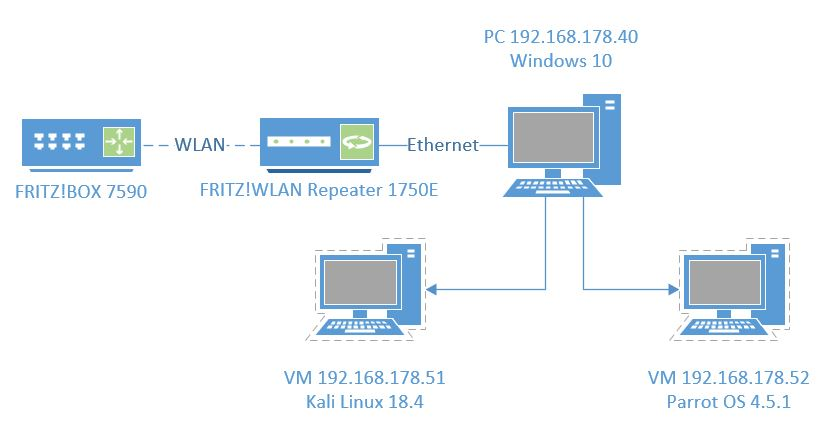
\includegraphics[width=0.9\textwidth]{Images/Visio}
    \caption[Testaufbau]{Testaufbau}
  \end{figure}
\section{Web Application Vulnerability Scanner (WVS)}
  \subsection{Auswahlkriterien}
  OWASP listet 50 verschiedene Tools zum Scannen von Webanwendungen auf
  \cite{OWASPtools}. Die Auswahl wurde auf WVS mit folgenden Eigenschaften eingegrenzt:
  \begin{itemize}
    \item 1. Free und Open Source WVS.
    \item 2. Kommerzielle WVS, die eine voll funktionsfähige Testversion anbieten.
    \item 3. WVS, deren aktuelles Release nicht älter als 2 Jahre ist oder innerhalb der letzten 2 Jahre modifiziert wurde.
    \item 4. WVS, die in der Lage sind, umfassende Scans auszuführen, um möglichst viele verschiedene Schwachstellenarten aufzuspüren.
  \end{itemize}
  Bei den bekanntesten Anbietern kommerzieller WVS wurde jeweils eine Testversion angefragt, um ein realistisches Abbild der aktuell meistgenutzten Tools zu erhalten und um die Ergebnisse der kostenlosen denen der kommerziellen Scanner gegenüber zu stellen. Es handelt sich um folgende Firmen:
  \\Acunetix, Beyond Security (WSSA), Beyond Trust (Retina), Netsparker, N-Stalker, Portswigger (BurpSuite Pro), Rapid 7 (Nexpose) und Tenable (Nessus).

  Von den angefragten Firmen stellten Acunetix, Netsparker, N-Stalker, Portswigger und Tenable jeweils eine Testversion zur Verfügung.

  \subsection{Ausgewählte WVS}
  Aus der Vielzahl der ursprünglich in Betracht kommenden WVS haben sich am Ende 9 herauskristallisiert, 5 mit einer OpenSource-Lizenz und 4 kommerzielle Produkte. Unter Punkt 4.2 werden sie im Zuge der Evaluation näher beschrieben.
    \subsubsection{Free und Open Source WVS}
      \begin{table}[H]
        \centering
          \begin{tabular}{|l|l|c|c|}
            \hline
            \textbf{WVS}              & \textbf{Entwickler}  & \textbf{Version}     & \textbf{Verwendete Plattform}  \\
            \hline
            \textbf{Arachni}          & Tasos Laskos         & 0.5.12 (WebUI)       & Windows                       \\
            \hline
            \textbf{Nikto}            & cirt.net             & 2.1.6                & Kali                          \\
            \hline
            \textbf{OpenVAS}          & Greenbone            & 7.0.3                & Parrot                        \\
            \hline
            \textbf{Wapiti}           & devloop              & 3.0.1                & Kali                          \\
            \hline
            \textbf{Zed Attack Proxy} & OWASP                & 2.7.0                & Parrot                        \\
            \hline
          \end{tabular}
        \caption[Ausgewählte Free und Open Source WVS]{Ausgewählte Free und Open Source WVS}
      \end{table}

    \subsubsection{Kommerzielle WVS}
      \begin{table}[H]
        \centering
          \begin{tabular}{|p{4cm}|l|c|c|}
            \hline
            \textbf{WVS}            & \textbf{Anbieter} & \textbf{Version} & \textbf{Verwendete Plattform}  \\
            \hline
            \textbf{Acunetix}       & Acunetix          & 12.0.190206130   & Windows/Kali                          \\
            \hline
            \textbf{Burp Suite Pro} & Portswigger       & 2.0.15           & Windows                       \\
            \hline
            \textbf{Nessus}         & Tenable           & 8.2.2            & Windows                       \\
            \hline
            \textbf{Netsparker}     & Netsparker        & 5.2.0.22027      & Windows                       \\
            \hline
          \end{tabular}
        \caption[Ausgewählte kommerzielle WVS]{Ausgewählte kommerzielle WVS}
      \end{table}
\newpage
  \subsection{Nicht ausgewählte WVS}
    Nachfoldend werden alle WVS aufgelistet, die als Kandidaten in Erwägung gezogen wurden, bei näherer Betrachtung jedoch nicht die erforderlichen Voraussetzungen erfüllten, um in die Evaluation aufgenommen zu werden.
    \subsubsection{Free und Open Source WVS}
    \begin{itemize}
      \item GoLismero \cite{GoLismero}: GoLismero ist ein in Python geschriebenes Framework, das verschiedene Penetrationtesting-Tools in sich vereint. Theoretisch sollten bei einem Angriff alle Tools angewendet und die jeweiligen Ergebnisse in einem einzigen Report gebündelt werden. In der Praxis hängte sich das Programm jedoch jedes Mal nach einer Weile auf, sowohl unter Kali-Linux und Parrot OS, als auch unter Windows. Es werden zwar Teilergebnisse auf dem Bildschirm angezeigt, dies reicht aber nicht aus, um in die Evaluation aufgenommen zu werden.
      \item Grabber \cite{Grabber}: Das von Romain Gaucher entwickelte Programm ist zwar noch Bestandteil von Kali-Linux, ist aber schon über 12 Jahre alt (Latest Release 2006).
      \item Grendel-Scan \cite{Grendel}: Seit 2013 gibt es auf dem SourceForge-Repository von David Byrne keine Veränderung.
      \item Iron Wasp \cite{Iron}: Die aktuelle Verison des Windows-Programms von Lavakumar Kuppan ist ein Beta-Release aus dem Jahr 2015.
      \item Ratproxy \cite{Ratproxy}: Die Entwicklung wurde 2009 von Google eingestellt.
      \item Skipfish \cite{Skipfish}: Ein weiteres Projekt von Google, das 2012 eingestellt wurde.
      \item SQLmap \cite{SQLmap}: SQLmap ist ein beliebtes Tool zum Auffinden von SQLi Schwachstellen, ist aber darauf beschränkt.
      \item Vega \cite{Vega}: Das aktuelle Release ist aus dem Jahr 2014, seit diesem Jahr wird in regelmäßigen Abständen angekündigt, ein Feature zum Exportieren der Ergebnisse hinzuzufügen, aber die Firma Subgraph scheint das Projekt nicht weiter zu verfolgen.
      \item Watobo \cite{Watobo}: Die letzte Änderung des OpenSource Scanners stammt aus dem Jahr 2015.
      \item Webscarab \cite{Webscarab}: Der Vorgänger von OWASPs Zed Attack Proxy ist veraltet (Latest Release 2011), OWASP empfiehlt, auf ZAP umzusteigen.
      \item Wfuzz \cite{Wfuzz}: Der in Python geschriebene Scanner verwendet die Bibliothek Pycurl für HTTP-Requests, diese unterstützt keine SSL/TLS Verschlüsselung.
      \item W3af \cite{W3af}: W3af wird zwar noch sporadisch mit Bibliotheks-Aktualisierungen gepflegt, das aktuelle Release ist jedoch aus dem Jahr 2014 und es ist weder auf Kali-Linux noch auf Parrot OS gelungen, alle für den Programmstart benötigten Dependencies zu installieren. Das bei der Installation generierte Script versucht, teils veraltete Module zu installieren, manuelles Nachinstallieren der aktuellen Versionen brachte keinen Erfolg.
      \begin{figure}[H]
        \centering
        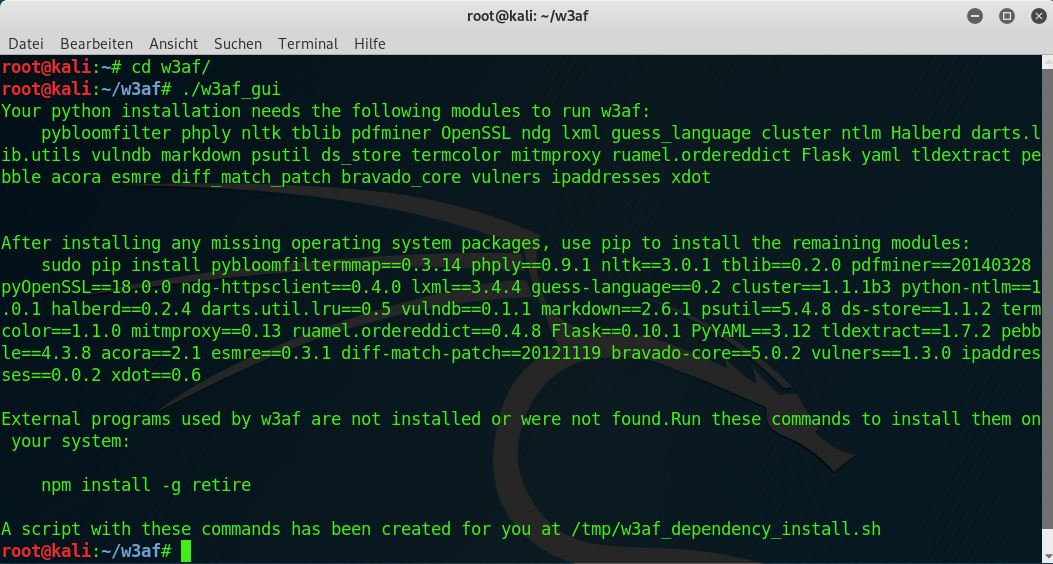
\includegraphics[width=0.9\textwidth]{Images/w3af}
        \caption[W3af: Fehlende Module]{W3af: Fehlende Module}
      \end{figure}
      \item Wikto \cite{Wikto}: Wikto ist eine Windows-Portierung von Nikto und bedarf daher keiner eigenen Evaluation.
      \item Xenotix \cite{Xenotix}: Xenotix wurde von OWASP für das Auffinden von Cross-Site-Scripting Schwachstellen entwickelt und ist darauf beschränkt.
    \end{itemize}
    \subsubsection{Kommerzielle WVS}
      \begin{itemize}
        \item N-Stalker \cite{Stalker}: Die angebotene ``7-Day Evaluation Licence'' erlaubt nur das Scannen einer einzigen, vorher festgelegten URL und ist daher für den geplanten Testaufbau nicht geeignet.
      \end{itemize}
\newpage
\section{Verwundbare Web-Applikationen}
  Bei der Auswahl der Web-Applikationen musste darauf geachtet werden, dass sie für WVS geeignet sind. Auf ursprünglich in die Auswahl aufgenommene Applikationen wie WebGoat, JuiceShop (beide von OWASP) oder Damn Vulnerable Web Application (Bestandteil von Metasploitable) wurde am Ende verzichtet, da hier beim Scannen keine hinreichenden Ergebnisse hervorgebracht wurden. Diese Anwendungen  sind zwar sehr gut dokumentiert, aber hauptsächlich für das Erlernen von manuellen Angriffen entwickelt worden. Es wurde bei der Auswahl auf das OWASP Vulnerable Web Applications Directory Project zurückgegriffen, das eine Reihe von verwundbaren Web-Applikationen auflistet \cite{OWASPWebApps}. Die Auswahl deckt mehrere Technologien wie PHP, ASP.Net oder HTML5 ab.

  Nachfolgend werden die für die Auswertung genutzten Web-Applikationen kurz vorgestellt.
  \begin{itemize}
    \item WA1: Altoro Mutual\\
    Altoro Mutual ist eine in C\texttt{\#} .NET geschriebene Online-Banking Web-Applikation, die von IBM entwickelt wurde, um WVS zu testen \cite{Altoro}.
    \item WA2: Webscantest\\
    Diese Web-Applikation ist in PHP geschrieben und wurde von NTOSpider entwickelt, um WVS zu testen. Die Schwachstellen sind direkt auf der Seite dokumentiert \cite{Webscantest}.
    \item WA3: Zero Bank\\
    Eine weitere Online-Banking Web-Applikation, entwickelt von Hewlett-Packard/Micro Focus \cite{Zero}.
    \item WA4: Bitcoin Web Site\\
    Diese von Netsparker entwickelte Applikation ist in ASP.NET geschrieben und simuliert eine Online-Seite für Bitcoin-Transaktionen \cite{Aspnet}.
    \item WA5: Acuart\\
    Eine Test-Seite von Acunetix, der einen Online-Shop für Kunstwerke simuliert, geschrieben in PHP \cite{Acuart}.
    \item WA6: Crack Me Bank\\
    Eine in PHP geschriebene Online-Banking Seite, entwickelt von Trustwave \cite{CrackMeBank}:
    \item WA7: Security Tweets\\
    Security Tweets ist eine von Twitter inspirierte Social Networks Applikation, die von Acunetix entwickelt wurde und HTML5 verwendet \cite{Tweets}.
 \end{itemize}
\chapter{Evaluation}
  \section{Gefundene Schwachstellen per Webanwendung}
   H, M, L und I: High, Medium, Low und Informational. Aus Gründen der Vergleichbarkeit wurden die Werte aus der zusätzlichen Kategorie ``Critical'' bei Nessus und Netsparker mit in die Kategorie High übernommen. WA1-7: Verwundbare Web-Applikationen.
    \begin{table}[H]
      \begin{tabular}{|r|c|c|c|c|c|c|c|c|c|c|c|c|c|c|}
        \cline{2-15}
        \multicolumn{1}{r|}{}       & \multicolumn{4}{c|}{\textbf{Arachni}} & \textbf{Nikto} & \multicolumn{4}{c|}{\textbf{OpenVAS}} & \textbf{Wapiti} & \multicolumn{4}{c|}{\textbf{ZAP}}  \\
        \cline{2-15}
        \multicolumn{1}{r|}{}       & H & M & L & I              &                & H & M & L & I              &                 & H & M & L & I                        \\
        \hline
        \textbf{WA1}      & 9    & 4    & 2   & 5                 & 12             & 0    & 2    & 0   & 24                & 10              & 1    & 2    & 5   & 0                           \\
        \hline
        \textbf{WA2}        & 4    & 10   & 5   & 29                & 18             & 0    & 8    & 0   & 41                & 12              & 1    & 4    & 11  & 0                           \\
        \hline
        \textbf{WA3}          & 4    & 6    & 4   & 4                 & 18             & 6    & 51   & 2   & 34                & 2               & 0    & 1    & 2   & 0                           \\
        \hline
        \textbf{WA4}    & 22   & 6    & 8   & 27                & 15             & 0    & 4    & 0   & 24                & 32              & 3    & 4    & 6   & 0                           \\
        \hline
        \textbf{WA5}             & 56   & 6    & 10  & 24                & 18             & 2    & 31   & 1   & 77                & 31              & 4    & 1    & 2   & 0                           \\
        \hline
        \textbf{WA6}      & 29   & 10   & 4   & 10                & 9              & 0    & 11   & 1   & 29                & 6               & 4    & 3    & 3   & 0                           \\
        \hline
        \textbf{WA7}    & 10   & 2    & 3   & 6                 & 7              & 1    & 31   & 1   & 77                & 0               & 0    & 1    & 5   & 0                           \\
        \hline
        \textbf{Subt.}           & 134  & 44   & 36  & 105               & 97             & 9    & 138  & 5   & 306               & 93              & 13   & 16   & 34  & 0                           \\
        \hline
        \textbf{Total}              & \multicolumn{4}{c|}{\textbf{319}}     & \textbf{97}    & \multicolumn{4}{c|}{\textbf{458}}     & \textbf{93}     & \multicolumn{4}{c|}{\textbf{63}}                \\
        \hline
      \end{tabular}
      \caption[Gefundene Schwachstellen der Open Source WVS]{Gefundene Schwachstellen der Open Source WVS}
    \end{table}

    \begin{table}[H]
      \begin{tabular}{|r|c|c|c|c|c|c|c|c|c|c|c|c|c|c|c|c|}
        \cline{2-17}
        \multicolumn{1}{l|}{}    & \multicolumn{4}{c|}{\textbf{Acunetix}}                   & \multicolumn{4}{c|}{\textbf{BurpSuite Pro}}          & \multicolumn{4}{c|}{\textbf{Nessus}}                  & \multicolumn{4}{c|}{\textbf{Netsparker}}                 \\
        \cline{2-17}
        \multicolumn{1}{c|}{}    & H            & M            & L           & I            & H           & M          & L           & I            & H           & M           & L          & I            & H            & M           & L           & I             \\
        \hline
        \textbf{WA1}   & 4            & 10           & 2           & 34           & 10          & 0          & 7           & 18           & 0           & 3           & 2          & 21           & 4            & 6           & 10          & 15            \\
        \hline
        \textbf{WA2}     & 25           & 41           & 6           & 14           & 5           & 2          & 4           & 160          & 1           & 7           & 1          & 25           & 37           & 18          & 24          & 20            \\
        \hline
        \textbf{WA3}       & 19           & 23           & 20          & 24           & 0           & 0          & 1           & 13           & 14          & 31          & 1          & 23           & 7            & 6           & 16          & 14            \\
        \hline
        \textbf{WA4} & 73           & 26           & 6           & 7            & 17          & 1          & 4           & 119          & 1           & 6           & 1          & 20           & 21           & 8           & 16          & 28            \\
        \hline
        \textbf{WA5}          & 39           & 34           & 9           & 19           & 28          & 0          & 4           & 49           & 21          & 18          & 1          & 21           & 24           & 18          & 12          & 12            \\
        \hline
        \textbf{WA6}   & 6            & 14           & 27          & 5            & 11          & 0          & 1           & 74           & 0           & 5           & 1          & 22           & 14           & 4           & 11          & 13            \\
        \hline
        \textbf{WA7} & 14           & 4            & 9           & 3            & 8           & 2          & 2           & 11           & 0           & 1           & 2          & 16           & 8            & 2           & 10          & 11            \\
        \hline
        \textbf{Subt.}        & \textbf{180} & \textbf{152} & \textbf{79} & \textbf{106} & \textbf{79} & \textbf{5} & \textbf{23} & \textbf{444} & \textbf{37} & \textbf{71} & \textbf{9} & \textbf{148} & \textbf{115} & \textbf{62} & \textbf{99} & \textbf{113}  \\
        \hline
        \textbf{Total}           & \multicolumn{4}{c|}{\textbf{517}}                        & \multicolumn{4}{c|}{\textbf{551}}                     & \multicolumn{4}{c|}{\textbf{265}}                     & \multicolumn{4}{c|}{\textbf{389}}                        \\
        \hline
      \end{tabular}
      \caption[Gefundene Schwachstellen der kommerziellen WVS]{Gefundene Schwachstellen der kommerziellen WVS}
    \end{table}

  \section{Bedienung, Reporting und Geschwindigkeit}
    \subsection{Open Source}
        \begin{itemize}
          \item Arachni \cite{Arachni}:\\
            Arachni gibt es als reine Terminal-Anwendung oder als Ruby on Rails Framework mit Web-Interface. Die Web-Oberfläche ist übersichtlich und verständlich aufgebaut, der User findet sich schnell zurecht und kann sofort mit dem Scannen einer Seite beginnen, die Scangeschwindigkeit ist überdurchschnittlich. Als Hilfestellung gibt es ein umfangreiches Wiki mit Erklärungen und Screenshots. Der Report ist sehr umfangreich, verschiedene Balken- und Kuchendiagramme geben Statistiken über Art und Schweregrad der Funde wieder, zudem gibt es Verlinkungen zu den OWASP Top 10 und detaillierte Ausführungen über die Schwachstellen. Arachni unterscheidet bei den Funden außerdem zwischen gesicherten (``Trusted'') und noch zu überprüfenden Ergebnissen (``Untrusted'').

            \textbf{Bewertung: Reporting 4, Bedienung 3, Geschwindigkeit 3}
            \begin{figure}[H]
              \centering
              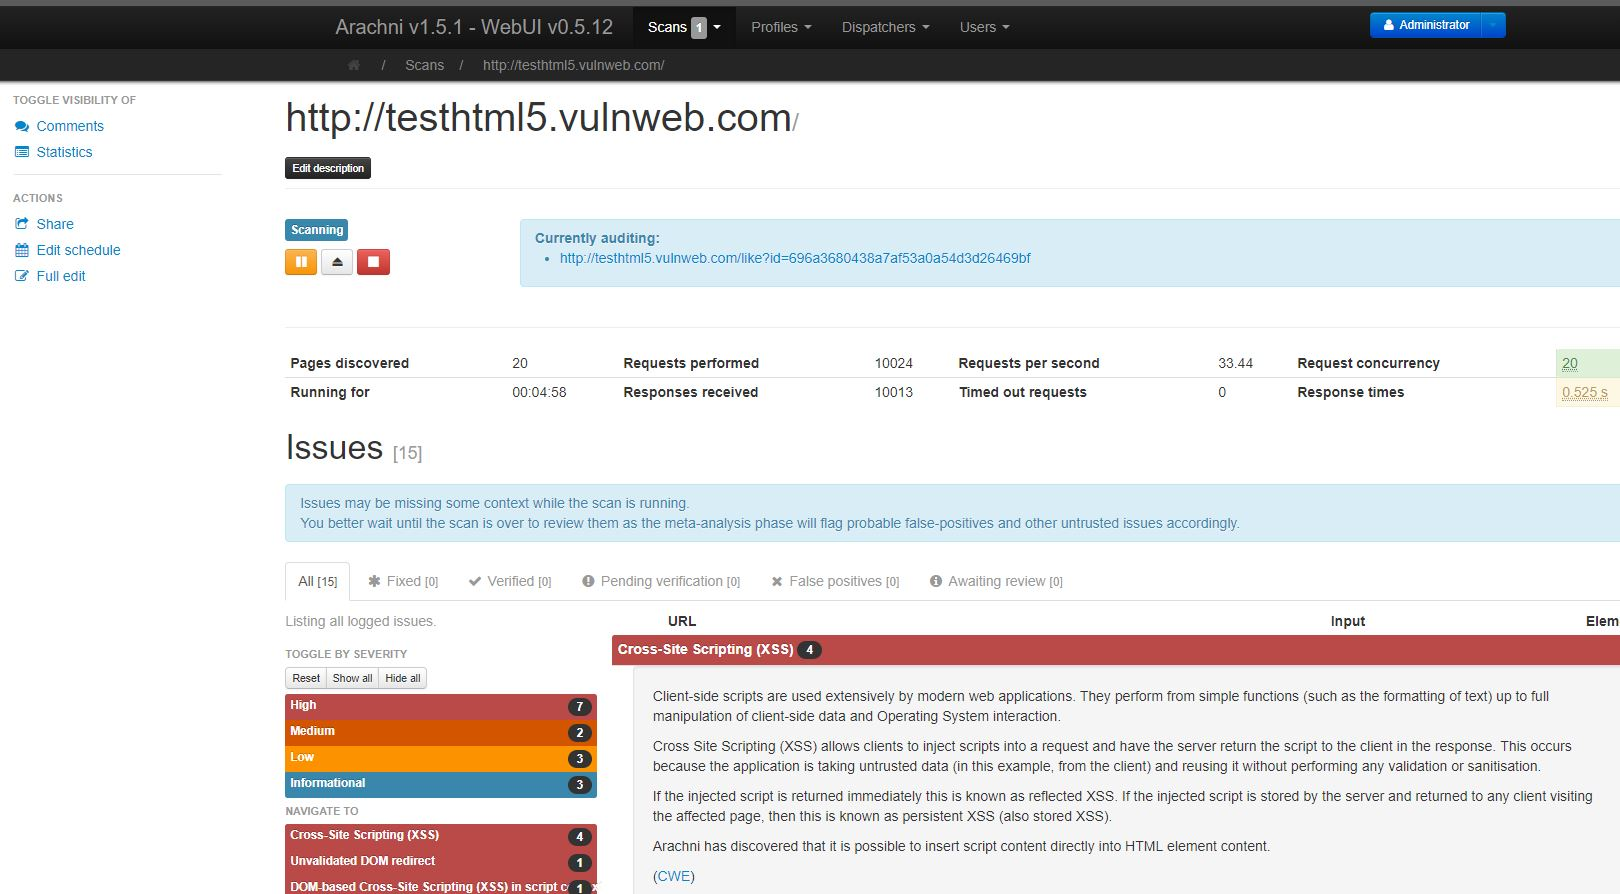
\includegraphics[width=0.9\textwidth]{Images/Arachni}
              \caption[Arachni WebUI 0.5.12]{Arachni WebUI 0.5.12}
            \end{figure}
          \item Nikto \cite{Nikto}:\\
            Nikto ist ein gut dokumentiertes Terminal-Programm, nach kurzer Einarbeitung hat ein ungeübter User die benötigten Befehle und Optionen gefunden, um einen Scan zu starten.
            Der generierte Report listet alle gefundenen Schwachstellen auf, unterscheidet diese jedoch im Gegensatz zu den meisten anderen WVS nicht zwischen High, Medium, Low und Informational. Die Scan-Geschwindigkeit ist über- durchschnittlich.

            \textbf{Bewertung: Reporting 1, Bedienung 2, Geschwindigkeit 3}
          \item OpenVAS \cite{OpenVAS}:\\
            OpenVAS ist aus der Software Nessus hervorgegangen, als diese im Jahr 2005 von Open Soucre zu einer kommerziellen Lizenz wechselte, und wird seitdem auf Basis der letzten freien Nessus-Version 2.2 von Greenbone Networks weiterentwickelt. Der Scanner ist eingebettet in den Greenbone Security Assistant, der über ein Web-Interface bedient wird. Die Oberfläche ist nicht selbsterklärend, es bedarf etwas an Recherche, bis sich dem User der logische Aufbau des Programms erschließt. Hier ist das ``Tech Doc-Portal'' von Greenbone sehr hilfreich. Zuerst muss unter Configuration/Targets ein Ziel definiert werden, dann kann der User für dieses Ziel unter dem Punkt ``Scans'' einen Task erstellen und diesen entweder sofort oder per Schedule starten.
            Die umständliche Handhabung hat jedoch den Vorteil, dass sich leicht mehrere Tasks automatisieren lassen. Der Bericht präsentiert sich etwas sparsam, die gefundenen Schwachstellen der Kategorie ``Informational'' werden nicht aufgelistet.

            \textbf{Bewertung: Reporting 2, Bedienung 1, Geschwindigkeit 2}
            \begin{figure} [H]
              \centering
              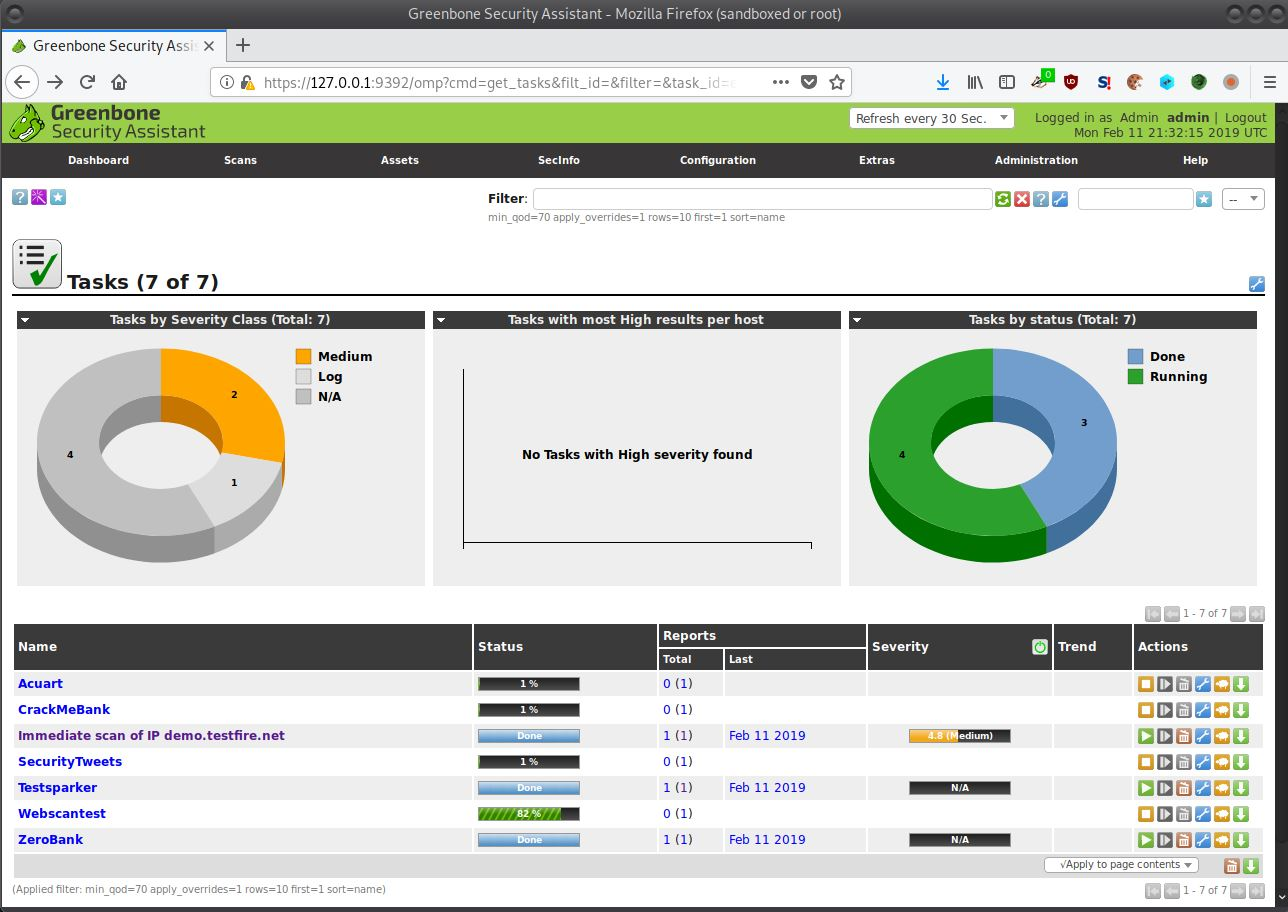
\includegraphics[width=0.85\textwidth]{Images/OpenVAS}
              \caption[OpenVAS im Greenbone Security Assistant]{OpenVAS im Greenbone Security Assistant}
            \end{figure}
          \item Wapiti \cite{Wapiti}:\\
            In der Handhabung und im Reporting ähnelt Wapiti dem anderen reinen Terminal-Programm Nikto. Die auswählbaren Optionen sind ähnlich, und die gefundenen Schwachstellen werden auch hier nicht in Kategorien eingeteilt. Die Dokumentation fällt etwas spartanischer aus, ist aber ausreichend, um sich schnell zurecht zu finden. Wapiti scannt fast so schnell wie Nikto und reiht sich hier auf dem dritten Platz ein.

            \textbf{Bewertung: Reporting 1, Bedienung 2, Geschwindigkeit 3}

          \item Zed Attack Proxy \cite{ZAP}:\\
            Der von OWASP entwickelte Scanner hat eine übersichtliche Benutzeroberfläche und lässt sich intuitiv bedienen. Auf der Startseite lässt sich direkt die anzugreifende URL eingeben und ohne weitere Konfiguration angreifen. Es gibt umfangreiche Hilfestellung in Form eines Handbuchs und einem Online-Wiki, zudem gibt es mit der OWASP ZAP User Group ein gut frequentiertes Benutzerforum, auf dem ein reger Austausch zwischen den Benutzern stattfindet.
            Auffällig sind die langen Scan-Zeiten von mehreren Stunden, die sich jedoch nicht in einer höheren Anzahl an gefundenen Schwachstellen widerspiegeln. Die wenigen Funde werden im Report ausführlich beschrieben einschließlich umfangreicher Empfehlungen zur Behebung.

            \textbf{Bewertung: Reporting 3, Bedienung 3, Geschwindigkeit 0}
          \begin{figure}[H]
            \centering
            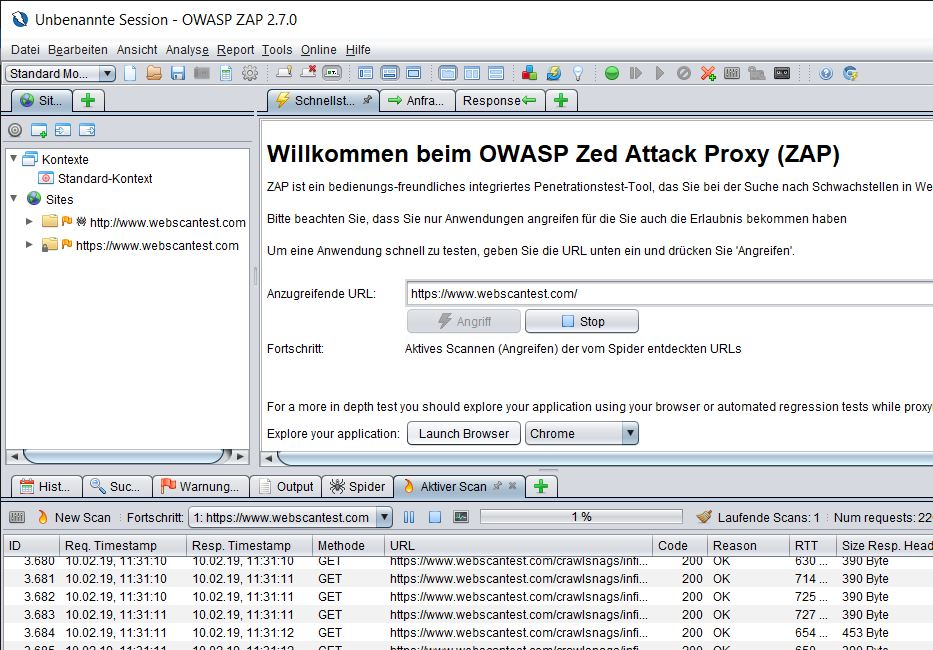
\includegraphics[width=0.9\textwidth]{Images/ZAP}
            \caption[Grafische Benutzeroberfläche von ZAP]{Grafische Benutzeroberfläche von ZAP}
          \end{figure}
        \end{itemize}

    \subsection{Kommerziell}
      \begin{itemize}
        \item Acunetix \cite{Acunetix}:\\
          Acunetix stellte eine 14-tägige Vollversion zur Verfügung. Die graphische Oberfläche ist sehr übersichtlich und lässt sich intuitiv bedienen. Online gibt es ein Support-Portal mit ausführlicher Dokumentation und Hilfestellung.
          Auffällig ist die im Vergleich zu allen anderen WVS ungewöhnlich hohe Scan-Geschwindigkeit, die sich im Minutenbereich einordnet.
          Unter Windows brachte Acunetix das System mehrmals zum Absturz (BSoD), so dass auf die Linux-Version ausgewichen wurde. Hier lief das Programm stabil und scannte von den kommerziellen WVS am schnellsten, von allen WVS muss sich Acunetix hier nur den Terminalprogrammen Wapiti und Nikto geschlagen geben. Der Report listet zu jeder gefundenen Schwachstelle sehr detailliert die vollständigen GET- und POST-Requests sowie teilweise seitenlange Code-Passagen auf. Die Empfehlungen zur Behebung der Funde könnten hingegen ausführlicher sein. Aufgrund der Abstürze wurden bei der Gesamtpunktzahl 3 Punkte abgezogen.

          \textbf{Bewertung: Reporting 3, Bedienung 3, Geschwindigkeit 4}\\

          \begin{figure}[H]
            \centering
            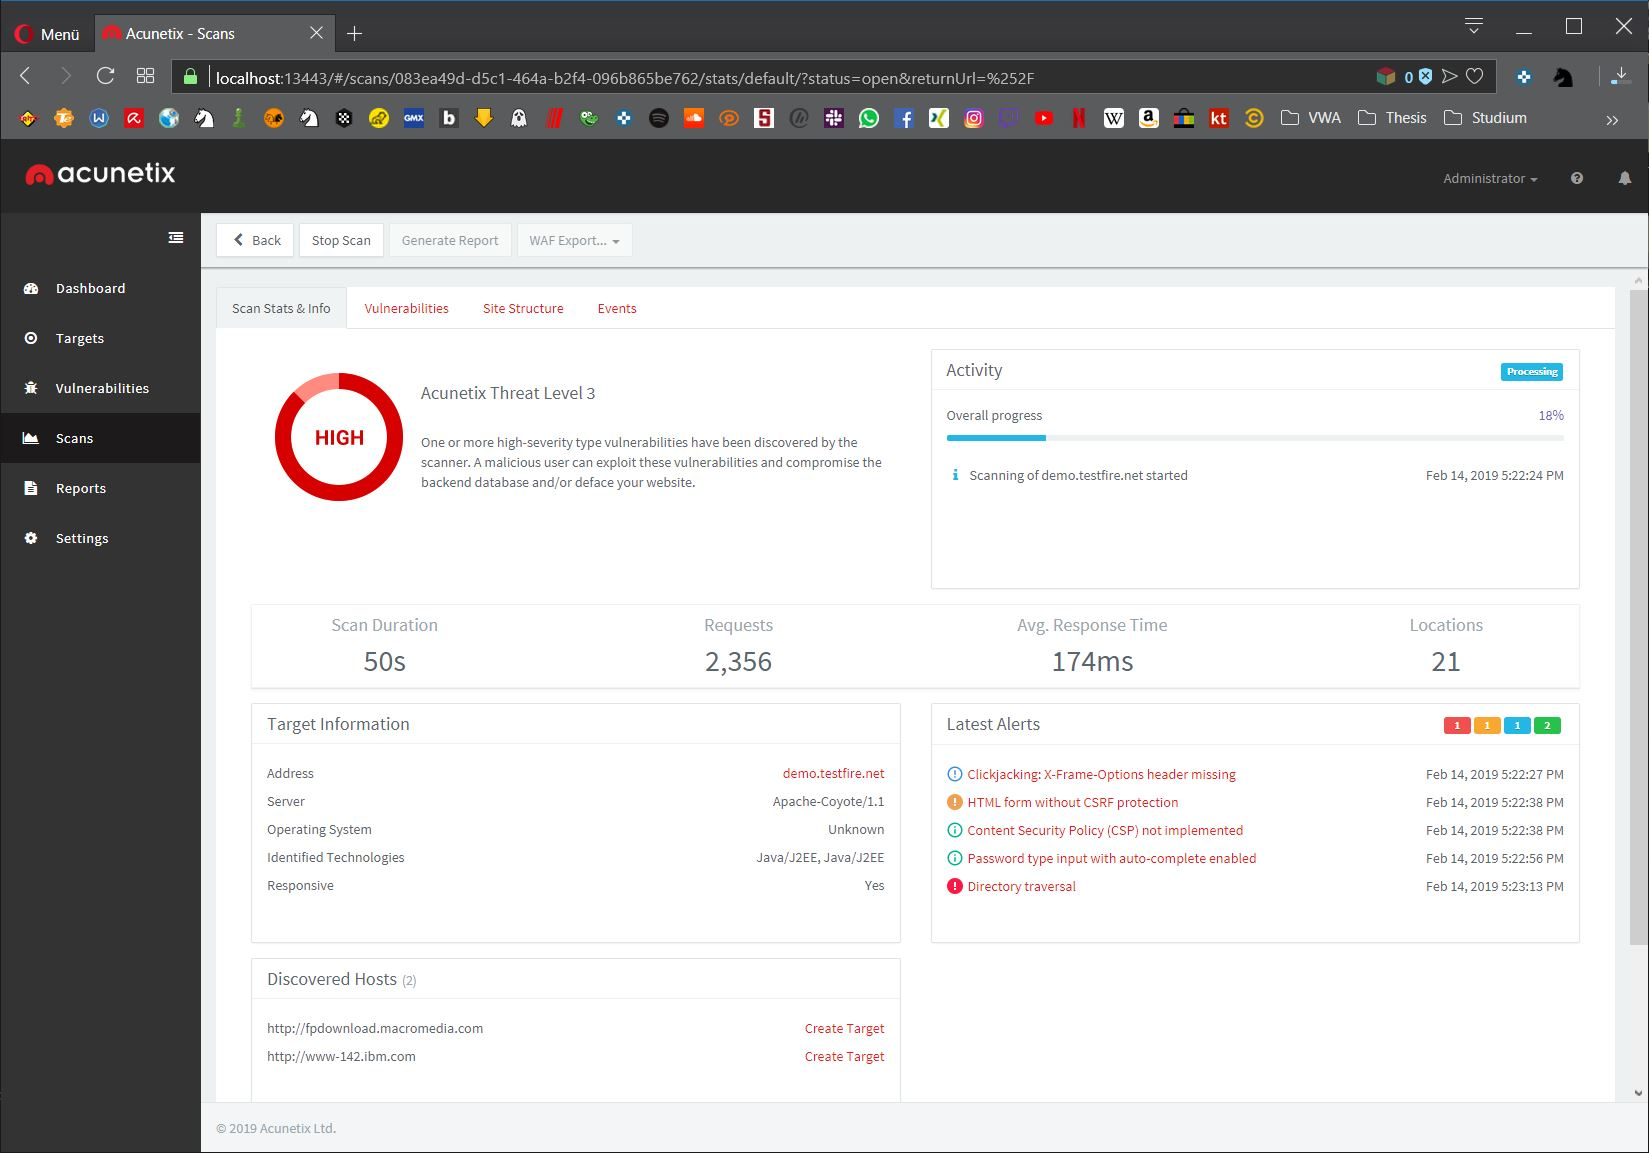
\includegraphics[width=0.9\textwidth]{Images/Acunetix}
            \caption[Weboberfläche von Acunetix]{Weboberfläche von Acunetix}
          \end{figure}
          \newpage
        \item BurpSuite Pro \cite{Burp}:\\
          Die Firma Portswigger stellte auf Anfrage eine 30-tägige unbeschränkte Testversion zur Verfügung.
          BurpSuite Pro enthält eine umfangreiche Dokumentation mit zahlreichen Hilfestellungen für verschiedene Anwendungsszenarien.  Das Dashboard ist sehr übersichtlich und intuitiv zu bedienen: mit Hilfe des Buttons ``New Scan'' lässt sich direkt ohne größeren Konfigurationsaufwand eine Website erfolgreich und in durchschnittlicher Geschwindigkeit scannen.
          \begin{figure}[H]
            \centering
            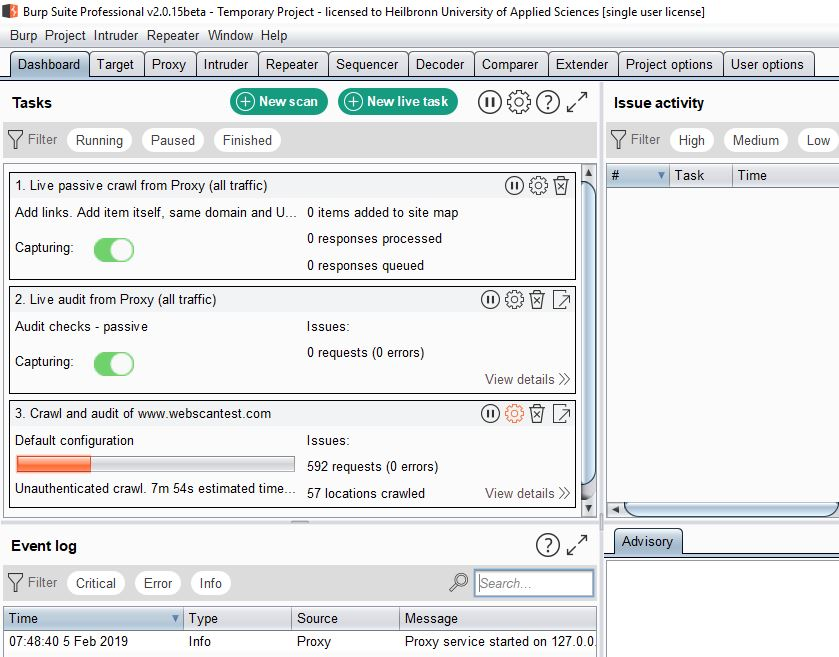
\includegraphics[width=0.91\textwidth]{Images/BurpSuitePro}
            \caption[Dashboard von BurpSuite Pro]{Dashboard von BurpSuite Pro}
          \end{figure}
          Der von BurpSuite generierte Report ist von allen getesteten WVS der umfangreichste und ist trotzdem sehr übersichtlich. Ähnlich wie Arachni unterscheidet BurpSuite zwischen gesicherten und ungesicherten Ergebnissen, allerdings noch genauer: in einer ``Confidence''-Tabelle wird zwischen gesicherten (Certain), wahrscheinlichen (Firm) und möglichen (Tentative) Schwachstellen unterschieden.

          \textbf{Bewertung: Reporting 4, Bedienung 3, Geschwindigkeit 2}
          \begin{figure}[H]
            \centering
            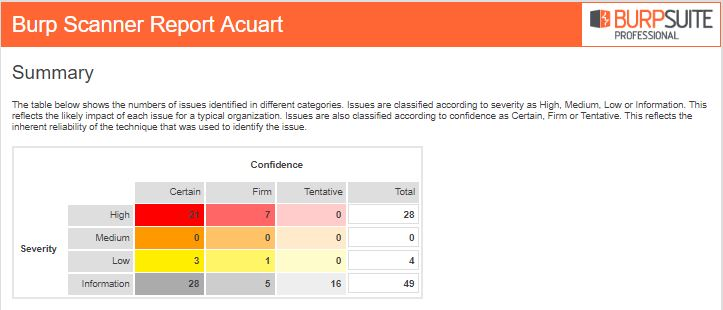
\includegraphics[width=0.76\textwidth]{Images/BurpReport}
            \caption[Confidence-Tabelle im Report von BurpSuite Pro]{Confidence-Tabelle im Report von BurpSuite Pro}
          \end{figure}

        \item Nessus \cite{Nessus}:\\
          Die Firma Tenable bietet zwei Testversionen an: Nessus Home für das Testen des heimischen Netzwerks, gültig für ein Jahr sowie eine unbeschränkte Version von Nessus Pro, gültig für sieben Tage.
          Nessus präsentiert sich auf einer übersichtlich gestalteten Web-Schnittstelle und ist selbsterklärend bedienbar. Einen Hilfe-Button sucht man vergeblich, die umfangreiche Dokumentation mit Anleitungen findet man online durch Recherchieren. Die Scangeschwindigkeit ist durchschnittlich, der Report übersichtlich aber eher spartanisch. Nur durch Anklicken der Funde gibt es online Beschreibungen und Lösungsvorschläge.

          \textbf{Bewertung: Reporting 2, Bedienung 3, Geschwindigkeit 2}
          \begin{figure}[H]
            \centering
            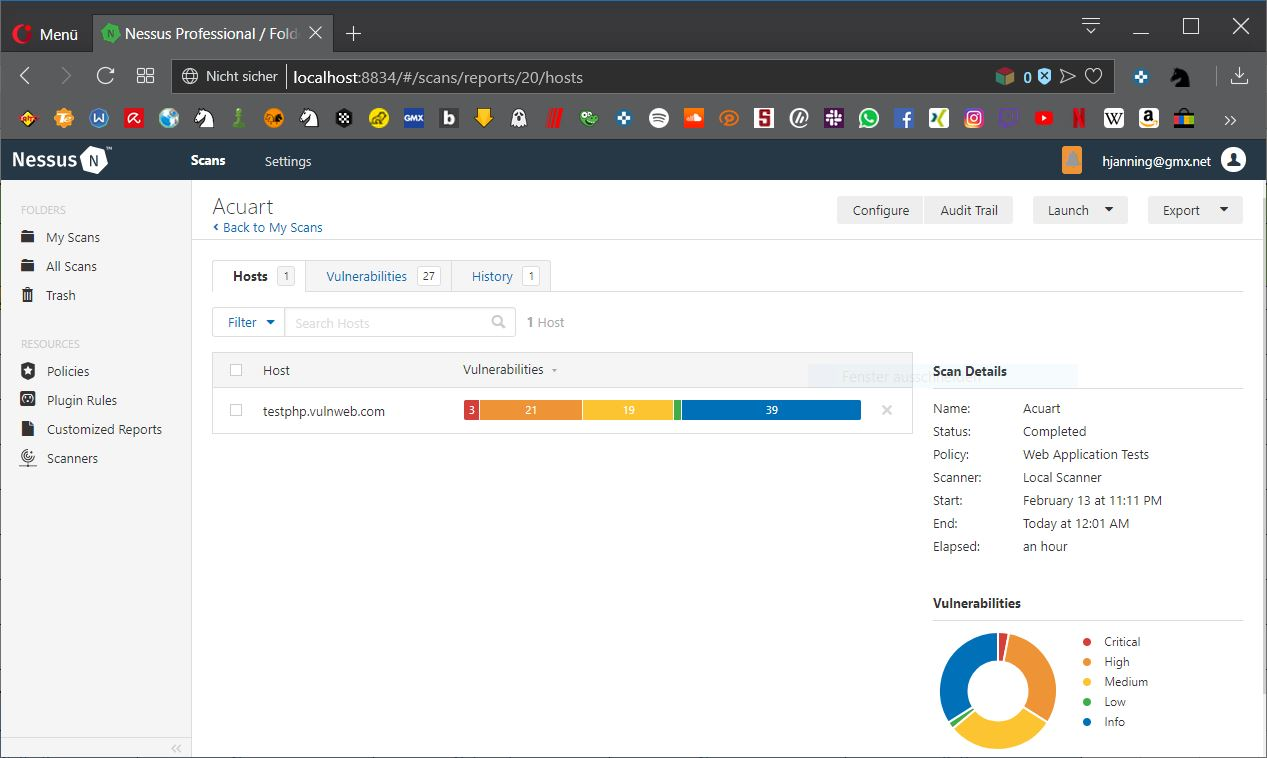
\includegraphics[width=0.9\textwidth]{Images/Nessus}
            \caption[Grafische Benutzeroberfläche von Nessus]{Grafische Benutzeroberfläche von Nessus}
          \end{figure}
        \item Netsparker \cite{Netsparker}:\\
          Netsparker stellte nach Rücksprache eine 14-tägige Testversion zur Verfügung, die auf 8 zu scannende Web-Applikationen begrenzt ist. Die grafische Benutzeroberfläche ist etwas unruhig und überladen, der User kann aber direkt über den Button ``New'' eine Web-Seite scannen. Die Scangeschwindigkeit ist im unteren Mittelfeld angesiedelt. Der Report ist äußerst umfangreich aber etwas unübersichtlich. Wie Nessus hat auch Netsparker nach High, Medium, Low und Informational eine fünfte Kategorie ``Critical'' eingeführt, die auf besonders kritische Schwachstellen hinweist. Wie bei Arachni und BurpSuite werden gesicherte Ergebnisse gesondert gekennzeichnet, hier als ``Confirmed''.

          \textbf{Bewertung: Reporting 3, Bedienung 2, Geschwindigkeit 1}
          \begin{figure}[H]
            \centering
            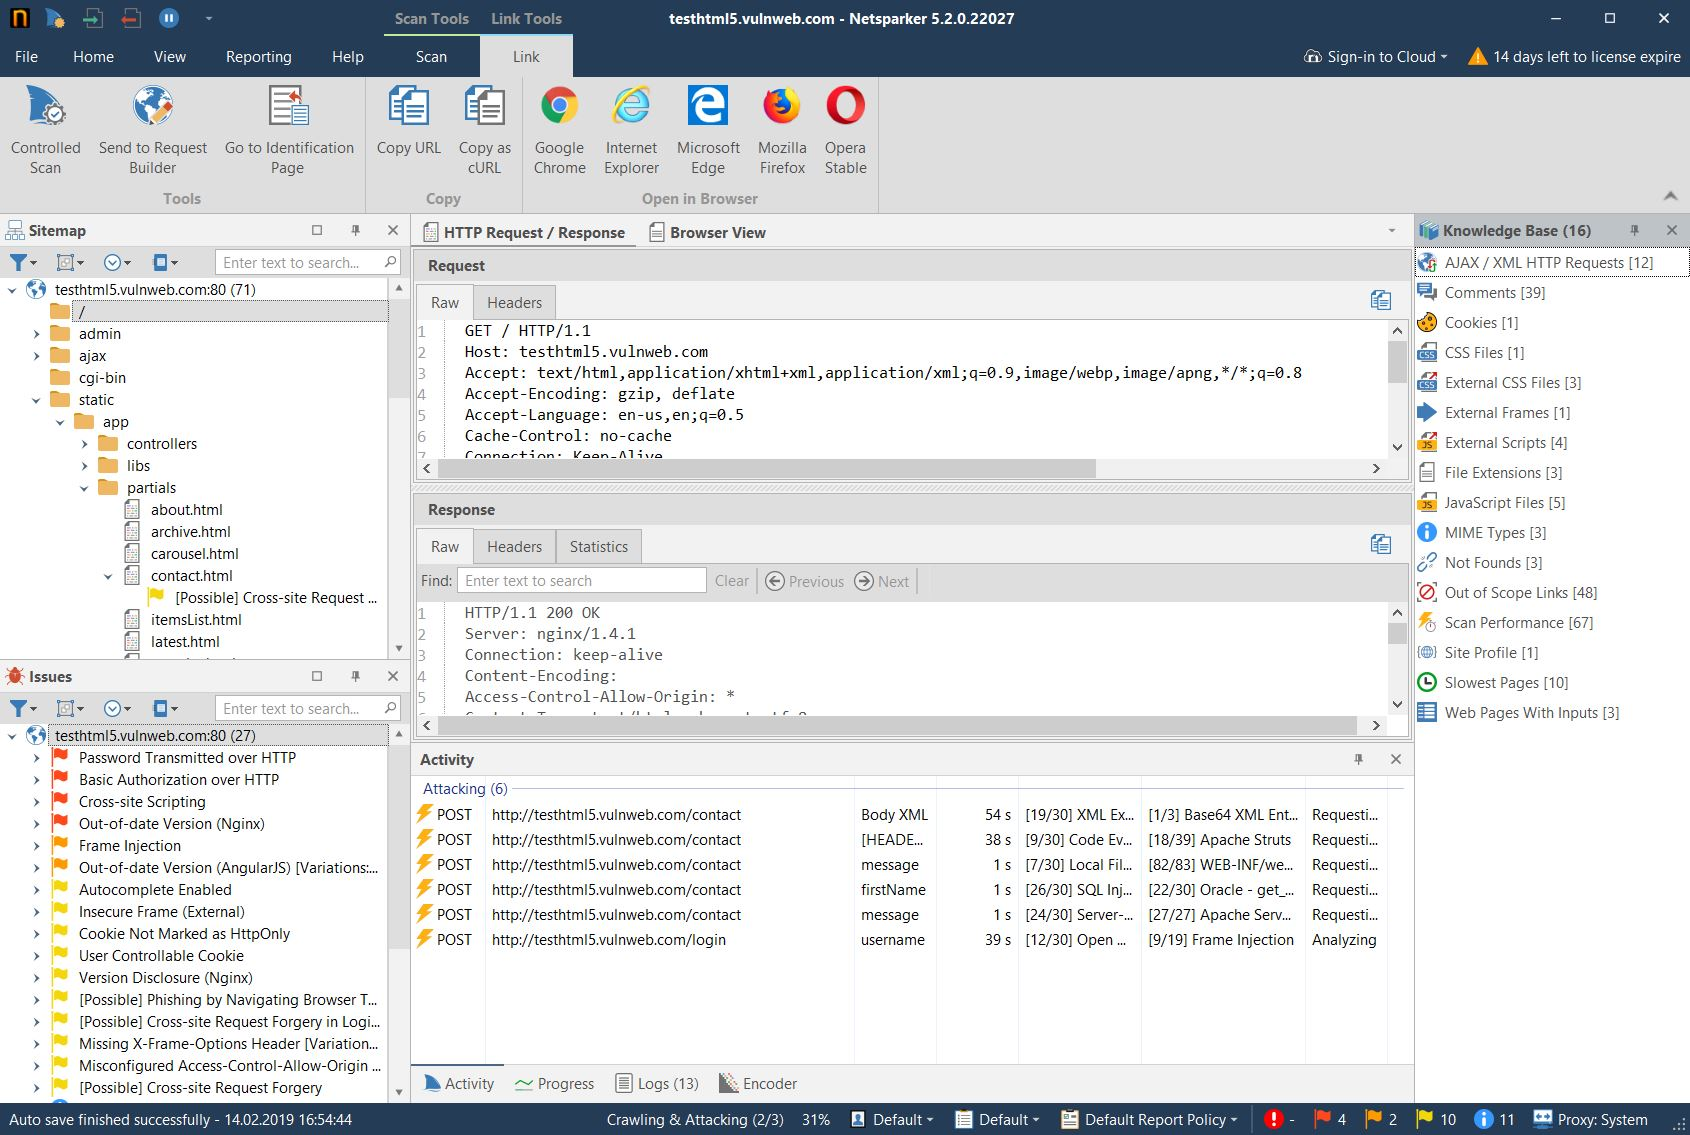
\includegraphics[width=0.9\textwidth]{Images/Netsparker}
            \caption[Grafische Benutzeroberfläche von Netsparker]{Grafische Benutzeroberfläche von Netsparker}
          \end{figure}
     \end{itemize}
\newpage
     \subsection{Scanzeiten}
     In den beiden folgenden Tabellen sind die Zeiten aufgeführt, die die WVS benötigten, um die jeweiligen Webanwendungen zu scannen.
     \paragraph{Open Source WVS}
     \
\begin{table}[H]
\begin{tabular}{|r|c|c|c|c|c|}
\hline
                            & \textbf{Arachni} & \textbf{Nikto} & \textbf{OpenVAS} & \textbf{Wapiti} & \textbf{Zed Attack Proxy}  \\
\hline
\textbf{Altoro Mutual}      & 41               & 96             & 38               & 88              & 615                        \\
\hline
\textbf{Webscantest}        & 86               & 80             & 90               & 82              & 821                        \\
\hline
\textbf{Zero Bank}          & 42               & 29             & 85               & 31              & 786                        \\
\hline
\textbf{Aspnet Testsparker} & 28               & 20             & 29               & 14              & 579                        \\
\hline
\textbf{Acuart}             & 39               & 9              & 43               & 23              & 660                        \\
\hline
\textbf{Crack Me Bank}      & 38               & 32             & 45               & 28              & 704                        \\
\hline
\textbf{Security Tweets}    & 28               & 19             & 33               & 27              & 523                        \\
\hline
\textbf{Total}              & \textbf{302}     & \textbf{285}   & \textbf{363}     & \textbf{293}    & \textbf{4688}              \\
\hline
\end{tabular}
\caption[Scanzeiten der Open Source WVS in Minuten]{Scanzeiten der Open Source WVS in Minuten}
\end{table}
\paragraph{Kommerzielle WVS}
\

\begin{table}[H]
\begin{tabular}{|r|c|c|c|c|}
\hline
                            & \textbf{Acunetix} & \textbf{Burp Suite Pro} & \textbf{Nessus} & \textbf{Netsparker}  \\
\hline
\textbf{Altoro Mutual}      & 15                & 56                      & 44              & 46                   \\
\hline
\textbf{Webscantest}        & 60                & 102                     & 82              & 241                  \\
\hline
\textbf{Zero Bank}          & 26                & 71                      & 68              & 47                   \\
\hline
\textbf{Aspnet Testsparker} & 11                & 30                      & 27              & 52                   \\
\hline
\textbf{Acuart}             & 6                 & 45                      & 61              & 37                   \\
\hline
\textbf{Crack Me Bank}      & 28                & 39                      & 31              & 71                   \\
\hline
\textbf{Security Tweets}    & 8                 & 41                      & 51              & 20                   \\
\hline
\textbf{Total}              & \textbf{154}      & \textbf{384}            & \textbf{364}    & \textbf{514}         \\
\hline
\end{tabular}
\caption[Scanzeiten der kommerziellen WVS in Minuten]{Scanzeiten der kommerziellen WVS in Minuten}
\end{table}


     \newpage
     \subsection{Gesamtbewertung und Ranking}
     \paragraph{Open Source WVS}
     \
       \begin{table}[H]
       \begin{tabular}{|r|c|c|c|c|c|}
       \hline
       \textbf{}            & \textbf{Arachni} & \textbf{Nikto} & \textbf{OpenVAS} & \textbf{Wapiti} & \textbf{ZAP}  \\
       \hline
       \textbf{Scanergebnis (50\%) *5}    & \textbf{3}      &  \textbf{1}      & \textbf{4}      &   \textbf{1}     &  \textbf{0}       \\
       \hline
       \textbf{Reporting (20\%) *2}       &  \textbf{4}     &  \textbf{1}      & \textbf{2}      &   \textbf{1}    &   \textbf{3}     \\
       \hline
       \textbf{Bedienung (20\%) *2}       & \textbf{3}       & \textbf{2}     & \textbf{1}       & \textbf{2}      & \textbf{3}        \\
       \hline
       \textbf{Geschwindigkeit (10\%)} & \textbf{3}       & \textbf{3}    & \textbf{2}       & \textbf{3}     & \textbf{0}          \\
       \hline
       \textbf{Gesamt}                 &   \textbf{32}     &  \textbf{14}   &  \textbf{28}      &  \textbf{14}    &  \textbf{12}          \\
       \hline
       \end{tabular}
       \caption[Bewertung der Open Source WVS]{Bewertung der Open Source WVS}
     \end{table}
     \paragraph{Kommerzielle WVS}
     \
       \begin{table}[H]
       \begin{tabular}{|r|c|c|c|c|}
       \hline
       \textbf{}       & \textbf{Acunetix} & \textbf{BurpSuite Pro} & \textbf{Nessus} & \textbf{Netsparker}  \\
       \hline
       \textbf{Scanergebnis (50\%) *5}    & \textbf{4}      &  \textbf{4}            & \textbf{2}      &   \textbf{3}         \\
       \hline
       \textbf{Reporting (20\%) *2}       &  \textbf{3}     &  \textbf{4}            & \textbf{2}      &   \textbf{3}         \\
       \hline
       \textbf{Bedienung (20\%) *2}       & \textbf{3}      & \textbf{3}           & \textbf{3}      & \textbf{2}        \\
       \hline
       \textbf{Geschwindigkeit (10\%)} & \textbf{4}       & \textbf{2}              & \textbf{2}      & \textbf{1}            \\
       \hline
       \textbf{Gesamt}                 &  \textbf{36}     & \textbf{36}              & \textbf{22}       &  \textbf{26}                    \\
       \hline
       \end{tabular}
       \caption[Bewertung der kommerziellen WVS]{Bewertung der kommerziellen WVS}
     \end{table}
     \paragraph{Ranking aller WVS}
     \
     \begin{table}[H]
  \begin{tabular}{|r|r|c|c|c|c|c|}
 \cline{2-7}
 \multicolumn{1}{l|}{} & \textbf{WVS}           & \textbf{Gesamt} & Scanergebnis & Reporting & Bedienung & Geschwindigkeit  \\
 \hline
 \textbf{1}            & \textbf{BurpSuite Pro} & \textbf{36}     & 4            & 4         & 3         & 2                \\
 \hline
 \textbf{2}            & \textbf{Acunetix}      & \textbf{33}\footnotemark     & 4            & 3         & 3         & 4                \\
 \hline
 \textbf{3}            & \textbf{Arachni}       & \textbf{32}     & 3            & 4         & 3         & 3                \\
 \hline
 \textbf{4}            & \textbf{OpenVAS}       & \textbf{28}     & 4            & 2         & 1         & 2                \\
 \hline
 \textbf{5}            & \textbf{Netsparker}    & \textbf{26}     & 3            & 3         & 2         & 1                \\
 \hline
 \textbf{6}            & \textbf{Nessus}        & \textbf{22}     & 2            & 2         & 3         & 2                \\
 \hline
 \textbf{7}            & \textbf{Nikto}         & \textbf{14}     & 1            & 1         & 2         & 3                \\
 \hline
 \textbf{7}            & \textbf{Wapiti}        & \textbf{14}     & 1            & 1         & 2         & 3                \\
 \hline
 \textbf{9}            & \textbf{ZAP}           & \textbf{12}     & 0            & 3         & 3         & 0                \\
 \hline
 \end{tabular}
 \caption[Ranking aller WVS]{Ranking aller WVS}
 \end{table}
 \footnotetext[1]{Ergebnis nach Abzug von 3 Punkten}

\chapter{Diskussion}
  \section{Anzahl der gefundenen Schwachstellen}
  Die Tabellen mit den gefundenen Schwachstellen zeigen eine große Bandbreite an unterschiedlichen Ergebnisssen. Während Zed Attack Proxy insgesamt nur 63 Schwachstellen findet, sind es bei BurpSuite Pro mit 551 Funden ungefähr neun mal so viele. Die beiden Terminalprogramme Nikto und Wapiti liegen fast gleich auf mit 97 und 93 Funden und sind damit nur geringfügig besser als das Schlusslicht Zed Attack Proxy.
  Mit 265 Funden hat Nessus bei den kommerziellen Scannern das schlechteste Ergebnis, überraschend ist hier vor allem, dass die Open Source Software und Nessus-Abspaltung OpenVAS fast 200 Schwachstellen mehr findet.
  OpenVAS lässt mit diesem Ergebnis auch noch den kommerziellen WVS Netsparker (389 Funde) hinter sich und belegt insgesamt den dritten Platz bei der Anzahl gefundener Schwachstellen. Arachni findet 319 Schwachstellen und reiht sich damit zwischen Nessus und Netsparker ein. Acunetix muss sich mit 517 Funden nur BurpSuite Pro geschlagen geben und belegt hier den zweiten Platz.

  Auch wenn die Werte in die Katgorien High, Medium, Low und Informational aufgesplittet werden, gibt es eine breite Palette an Ergebnissen, es gibt fast keinerlei Überein- stimmungen oder erkennbare Muster. Bei den WVS, die bei den insgesamt gefundenen Schwachstellen ungefähr gleich auf liegen, lässt sich dies veranschaulichen: Acunetix hat zum Beispiel mehr als 330 Funde in High und Medium eingeteilt und ca. 180 in Low und Informational, BurpSuite Pro stuft die Schwachstellen als nicht so schwerwiegend ein,  gerade einmal 84 Funde finden sich in High und Medium, aber 467 in Low und Informational. Arachni hat 134 Funde in die Kategorie High eingestuft, Nessus nur 37 und OpenVAS gar nur neun.

  Selbst wenn man die Ergebnisse nach den verwundbaren Webanwendungen aufteilt, gibt es keine Wiedererkennungswerte, weder gibt es eine Webseite, bei der von allen WVS besonders viele Schwachstellen gefunden wurden, noch sticht eine mit besonders wenigen Funden heraus. Auch die Anzahl der Funde pro Webanwendung ist von WVS zu WVS sehr verschieden. So findet zum Beispiel Acunetix auf der Seite Zero Bank (WA3) 68 Schwachstellen, BurpSuite Pro nur 14, andererseits findet BurpSuite Pro auf Webscantest (WA2) 169 Schwachstellen und Acunetix nur 86. OpenVAS findet auf Security Tweets (WA7) 110 Schwachstellen, Netsparker nur 31. Auf Webscantest (WA2) hingegen findet Netsparker doppelt so viele (99) Schwachstellen wie OpenVAS (49).\\
  Bezüglich der Webanwendungen gibt es eine interessante Beobachtung:  Acuart (WA5) und Security Tweets (WA7) wurden beide von Acunetix entwickelt, die naheliegende Vermutung, dass der WVS von Acunetix hier besonders viele Schwachstellen finden müsste, hat sich nicht bestätigt.
  Ebensowenig findet auch Netsparker auf der selbst entwickelten Bitcoin Web Site (WA4) relevant mehr Schwachstellen als die anderen WVS, Acunetix und BurpSuite Pro finden sogar deutlich mehr.

  Zusammenfassend muss festgehalten werden, dass bei der Anzahl der gefundenen Schwachstellen keinerlei Regelmäßigkeiten erkennbar sind, und so lässt sich die erste Forschungsfrage \textbf{Wie viele Schwachstellen werden von den WVS gefunden?} nur mit einem Blick auf die Tabelle beantworten - in absoluten Zahlen pro WVS.

  \section{Bedienung, Reporting und Scan-Geschwindigkeit}
  Dieses Kapitel widmet sich der Fragestellung \textbf{Wie unterscheiden sich die WVS in den Kategorien Bedienung, Reporting und Scan-Geschwindigkeit?}
  \subsection{Bedienung}
  In dieser Kategorie gibt es keinen WVS, der die volle Punktzahl erreicht, es gibt aber auch keinen mit null Punkten. Den beiden Terminalprogrammen Nikto und Wapiti fehlt es naturgemäß am Komfort, den eine grafische Benutzeroberfläche bietet, trotzdem schneiden sie noch besser ab als OpenVAS, das erst nach umfangreicher Einarbeitungszeit sinnvoll genutzt werden kann. Das Streben nach Automatisierung geht hier zu Lasten der Bedienbarkeit. Netsparker befindet sich mit seiner überladenen Benutzeroberfläche ebenfalls nur im Mittelfeld, Acunetix, BurpSuite Pro und Nessus sind - erwartungsgemäß für kommerzielle WVS - sehr übersichtlich und benutzerfreundlich.
  Die Open Source Programme Arachni und Zed Attack Proxy stehen dem jedoch in nichts nach und sind ebenfalls leicht verständlich und intuitiv zu bedienen. \\
  Insgesamt gibt es in dieser Kategorie keinen klaren Sieger, mit Ausnahme von OpenVAS sind alle WVS mühelos und unproblematisch zu bedienen.
  \subsection{Reporting}
  Nikto und Wapiti schneiden in dieser Kategorie unterdurchschnittlich ab, da sie die gefundenen Schwachstellen nicht nach Schweregrad unterteilen. Das Reporting von Nessus und OpenVAS könnte ausführlicher sein, OpenVAS verzichtet auf die Nennung von gefundenen Schwachstellen der Kategorie ``Informational'', bei Nessus sind die Beschreibungen der Schwachstellen und Lösungsvorschläge nur online abzurufen, das bedeutet zusätzlichen Aufwand, wenn der Auftraggeber einen gedruckten Bericht wünscht.
  Überdurchschnittlich schneiden Zed Attack Proxy, Acunetix und Netsparker ab, die alle sehr umfangreiche Beschreibungen der Schwachstellen liefern, Netsparker ist hier hervorzuheben für die zusätzliche Kategorie ``Critical'' und die besondere Kennzeichnung gesicherter Ergebnisse als ``Confirmed''.
  Überragende Ergebnisse liefern Arachni und BurpSuite Pro, Arachni sticht neben der Unterscheidung zwischen gesicherten und noch zu überprüfenden Ergenissen mit seinen ausführlichen Statistikfunktionen heraus, BurpSuite Pro mit seiner ``Confidence''-Tabelle, die die Schwachstellen noch genauer zwischen gesichert, wahrscheinlich und tentativ differenziert. Zudem bieten beide äußerst detaillierte Beschreibungen der Schwachstellen und sind trotzdem sehr übersichtlich gestaltet.
  \subsection{Scan-Geschwindigkeit}
  Mit einer Ausnahme liegen die Scan-Geschwindigkeiten alle im vertretbaren Bereich, Lediglich Zed Attack Proxy weicht hier mit Scanzeiten von 10 bis 14 Stunden pro Webanwendung ungewöhnlich weit von der Norm ab. Selbst die Werte von Netsparker, der auf dem vorletzten Platz landet, sind bis auf einen Ausreißer bei Webscantest (WA2) akzeptabel. Die Zeiten von OpenVAS, BurpSuite Pro und Nessus liegen alle nah beieinander und ordnen sich im Mittelfeld ein. Arachni sowie die beiden Terminalprogramme Nikto und Wapiti scannen überdurchschnittlich schnell, der beste WVS in dieser Kategorie ist mit großem Vorsprung Acunetix, der teilweise keine zehn Minuten für einen Scan benötigt.
  \section{Ranking}
  Die Ranking-Tabelle zeigt einen klaren Verlierer dieser Evaluation: Zed Attack Proxy ist der einzige WVS, der mit null Punkten bewertet werden musste, und das gleich zweimal, in den Kategorien Scanergebnis und Geschwindigkeit. Zed Attack Proxy ist damit als unbrauchbar zu bezeichnen, zumindest in der Funktion als WVS; die jeweils drei Punkte in den Kategorien Reporting und Bedienung sind wertlos, da kaum Schwachstellen gefunden werden. Nikto und Wapiti liegen mit jeweils 14 Punkten auf dem vorletzten Platz, mit den dürftigen Scanergebnissen und den Mängeln im Reporting sind diese Tools für professionelles Penetration Testing nur sehr bedingt tauglich. Nessus befindet sich mit 22 Punkten im unteren Mittelfeld und kann nur in der Kategorie Bedienung überzeugen, erfüllt aber insgesamt seinen Zweck. Netsparker hat gute Werte im Scanergebnis und im Reporting und belegt mit 26 Punkten den 5. Platz. OpenVAS erreicht 28 Punkte und lässt damit den kommerziellen WVS Nessus, aus dem OpenVAS hervorgegengen ist, hinter sich.
  Auf den ersten drei Plätzen befinden sich mit Arachni, Acunetix und BurpSuite Pro diejenigen WVS, die durchweg überdurchschnittliche und überragende Werte erreicht haben und somit fast uneingeschränkt empfehlenswert sind. Arachni belegt mit 32 Punkten den 3. Platz und ist damit der beste Open Source WVS.
  Acunetix belegt mit 33 Punkten den 2. Platz, allerdings nur durch den Punktabzug aufgrund der Abstürze beim Testen unter Windows. Ohne Abstürze hätte Acunetix sich den ersten Platz mit BurpSuite Pro geteilt.\\
  Testsieger und damit die Antwort auf die Frage \textbf{Welcher WVS schneidet insgesamt am besten ab?} ist BurpSuite Pro mit 36 Punkten. Ausschlaggebend für das Ergebnis sind in erster Linie das Scanergebnis und das Reporting, in beiden Kategorien hat BurpSuite Pro am besten von allen WVS abgeschnitten.

  \section{Open Source im Vergleich mit kommerziellen WVS}
  Nachfolgend wird die Frage \textbf{Wie schneiden die Open Source WVS im Vergleich mit kommerziellen WVS ab?} erörtert.

  Von den fünf getesteten Open Source WVS finden sich im Ranking drei auf den letzten Plätzen wieder. Nikto und Wapiti haben als Terminalprogramme naturgemäß Nachteile in der Handhabung, sie schneiden aber auch beim Scanergebnis und im Reporting unterdurchschnittlich ab. Zed Attack Proxy auf dem letzten Platz ist zwar als WVS ungeeignet, wird in der Regel aber auch als ``Intercepting Proxy'' verwendet, der den Browsertraffic abfangen, überprüfen und verändern kann. Der Name deutet darauf hin, dass dies die Hauptfunktion von Zed Attack Proxy ist, vom schlechten Abschneiden als WVS sollte hier also nicht auf die übrigen Funktionen geschlossen werden.\\
  Arachni und OpenVAS auf dem 3. und 4. Platz im Gesamtranking schneiden besser ab, als die kommerziellen WVS Netsparker und Nessus und stellen damit zwei kostengünstige Alternativen dar. Nach Bewältigung der Einarbeitungszeit lassen sich mit OpenVAS gute Ergebnisse erzielen, insbesondere wenn man einen hohen Automatisierungsgrad anstrebt.
  Arachni überzeugt mit leichter Handhabung, sehr gutem Reporting und überdurchschnittlicher Geschwindigkeit, bei der Anzahl der gefundenen Schwachstellen setzen sich jedoch die kommerziellen WVS BurpSuite Pro und Acunetix durch.


\chapter{Fazit und Ausblick}
Das Ziel dieser dieser Arbeit war es, aus der großen Anzahl von WVS die für eine Evaluation geeigneten herauszufiltern und auf ihre Tauglichkeit und Qualität zu testen. Nach eingehender Prüfung der in Frage kommenden Kandidaten wurden schließlich neun in die Evaluation aufgenommen, fünf Open Source- und vier kommerzielle WVS.
Zum Testen wurden sieben verwundbare Webanwendungen mit verschiedenen Technoligien ausgewählt, die von den WVS gescannt und auf Schwachstellen überprüft wurden. Anhand eines Punktesystems wurden die WVS in den Kategorien Scanergebnis, Reporting, Bedienung und Geschwindigkeit verglichen.\\
Neben dem Aufzeigen der Unterschiede in den einzelnen Kategorien, sollten die Fragen beantwortet werden, welcher WVS das beste Resultat erzielt und wie die Open Source WVS im Vergleich mit den kommerziellen Scannern abschneiden.

Durch die Evaluation gelang es, für jede Fragestellung Antworten zu finden:
\paragraph{Anzahl gefundener Schwachstellen:}
Mit Hilfe einer Tabelle wurden die großen Unterschiede bei der Anzahl gefundener Schwachstellen sichtbar gemacht, hier schnitten BurpSuitePro und Acunetix mit über 500 Funden am besten ab.
\paragraph{Bedienung, Reporting und Geschwindigkeit:}
Die Scan-Geschwindigkeit wurde den Berichten entnommen oder manuell ermittelt. Die subjektiven Eindrücke für die Bedienung und das Reporting wurden für jeden WVS einzeln beschrieben und mit Hilfe des Punktesystems bewertet. Die Bewertung resultiert in einem Gesamtranking.
\paragraph{Ranking:} Aus dem Gesamtranking lässt sich der WVS ermitteln, der am besten abgeschnitten hat, es ist BurpSuite Pro mit 36 Punkten.
\paragraph{Open Source im Vergleich mit kommerziellen WVS:}
Anhand des Rankings wurde auch das Abschneiden der Open Source WVS aufgezeigt, mit Arachni und OpenVAS an dritter und vierter Stelle der Rangliste gibt es vollwertige, kostenlose Alternativen zu den kommerziellen WVS.

Ungeachtet der Resultate soll hier jedoch durch Reflexion der gewählten Methodik auch auf die Grenzen der Evaluation eingegangen werden.\\
So hat die Gesamtanzahl der gefundenen Schwachstellen zum Beispiel nur eingeschränkte Aussagekraft; zum einen müsste jeder Fund noch durch manuelles Testen verifiziert werden, um False-Positives auszuschließen, zum anderen ist die durch die WVS vorgenommene Einteilung in die Kategorien ``High'', ``Medium'', ``Low'' und ``Informational'' problematisch, da die ``Informational''-Funde, wie der Name schon sagt, nur der Information dienen und gar kein Eingreifen erfordern. Würde man diese Werte ausblenden, ergäbe sich im Ranking ein komplett anderes Bild, der Testsieger BurpSuite Pro käme zum Beispiel nur noch auf 107 gefundene Schwachstellen und würde damit in dieser Kategorie den vorletzten Rang belegen. In diesem Zusammenhang muss rückblickend auch die Gewichtung der einzelnen Kategorien hinterfragt werden, angesichts der zweifelhaften Ausssagekraft des Scanergebnisses ist die Gewichtung von 50\% vielleicht zu hoch angesetzt. \\
Die Ergebnisse dieser Thesis sind somit als Grundlage für weitergehende Evaluationen einzuordnen.

Für künftige Studien sind mehrere Ansätze möglich:
\begin{itemize}
  \item Durch Verifizierung der False-Positives werden die Scan-Ergebnisse genauer, hier müsste allerdings aufgrund des hohen Aufwands die Anzahl der WVS und der Webanwendgen reduziert werden.
  \item Durch Weglassen der ``Informational''-Funde werden nur relevante Schwachstellen erfasst, die auch tatsächlich ein Eingreifen erfordern.
  \item Bei Auswahl und Gewichtung der Bewertungskategorien können andere Prioritäten gesetzt werden, indem etwa die Scan-Geschwindigkeit vernachlässigt oder bei den kommerziellen WVS der Preis mit einbezogen wird.
\end{itemize}
Des Weiteren sei hier für tiefergehende Analysen auf das Projekt OWASP-Benchmark \cite{OWASPbench} verwiesen, eine von OWASP entwickelte, kostenlose Testsuite, mit der WVS in mehrtägigen Scans anhand von tausenden von Testfällen untersucht werden können.







%%%%%%%%%%%%%%%%%%%
%% create listings list
%%%%%%%%%%%%%%%%%%%
%\lstlistoflistings
%\addcontentsline{toc}{chapter}{Listings}

\cleardoublepage
\phantomsection
\addcontentsline{toc}{chapter}{Quellenverzeichnis}
\printbibliography[title=Quellenverzeichnis]

\appendix
  \addtocontents{toc}{\protect{\vspace{3ex}}}
  \addtocontents{toc}{\protect\contentsline{chapter}{\appendixname}{}{}}
  %\addcontentsline{toc}{chapter}{Anhang}
  \chapter{Verwendete Abk"urzungen}
  \textbf{BSI} - Bundesamt für Sicherheit in der Informationstechnik

  \textbf{BSoD} - ``Blue Screen of Death'' (Kritischer Systemfehler unter Microsoft-Windows)

  \textbf{CGI} - Common Gateway Interface

  \textbf{CPU} - Central Processing Unit

  \textbf{CVE} - Common Vulnerabilities and Exposures

  \textbf{DAST} - Dynamic Application Security Testing

  \textbf{DoS} - Denial of Service

  \textbf{HTML} - Hypertext Markup Language

  \textbf{HTTP} - Hypertext Transfer Protocol

  \textbf{HTTPS} - Hypertext Transfer Protocol Secure

  \textbf{JSP} - JavaServer Pages

  \textbf{LDAP} - Lightweight Directory Access Protocol

  \textbf{NTLM} - New Technology Lan Manager

  \textbf{OS} - Operating System

  \textbf{OWASP} - The Open Web Application Security Project

  \textbf{RAM} - Random-Access Memory

  \textbf{REST} - Representational State Transfer

  \textbf{SAST} - Static Application Security Testing

  \textbf{SCA} - Static Code Analysis

  \textbf{SPA} - Single Page Application

  \textbf{SSL} - Secure Sockets Layer

  \textbf{SQL} - Structured Query Language

  \textbf{TLS} - Transport Layer Security

  \textbf{URI} - Uniform Resource Identifier

  \textbf{URL} - Uniform Resource Locator

  \textbf{WAF} - Web Application Firewall

  \textbf{WASC} - Web Application Security Consortium

  \textbf{WVS} - Web Application Vulnerability Scanner

  \textbf{WWW} - World Wide Web

  \textbf{XML} - Extensible Markup Language

  \textbf{XSS} - Cross Site Scripting
  \newpage

  \chapter{Screenshots}
  \begin{figure}[htb!]
    \centering
      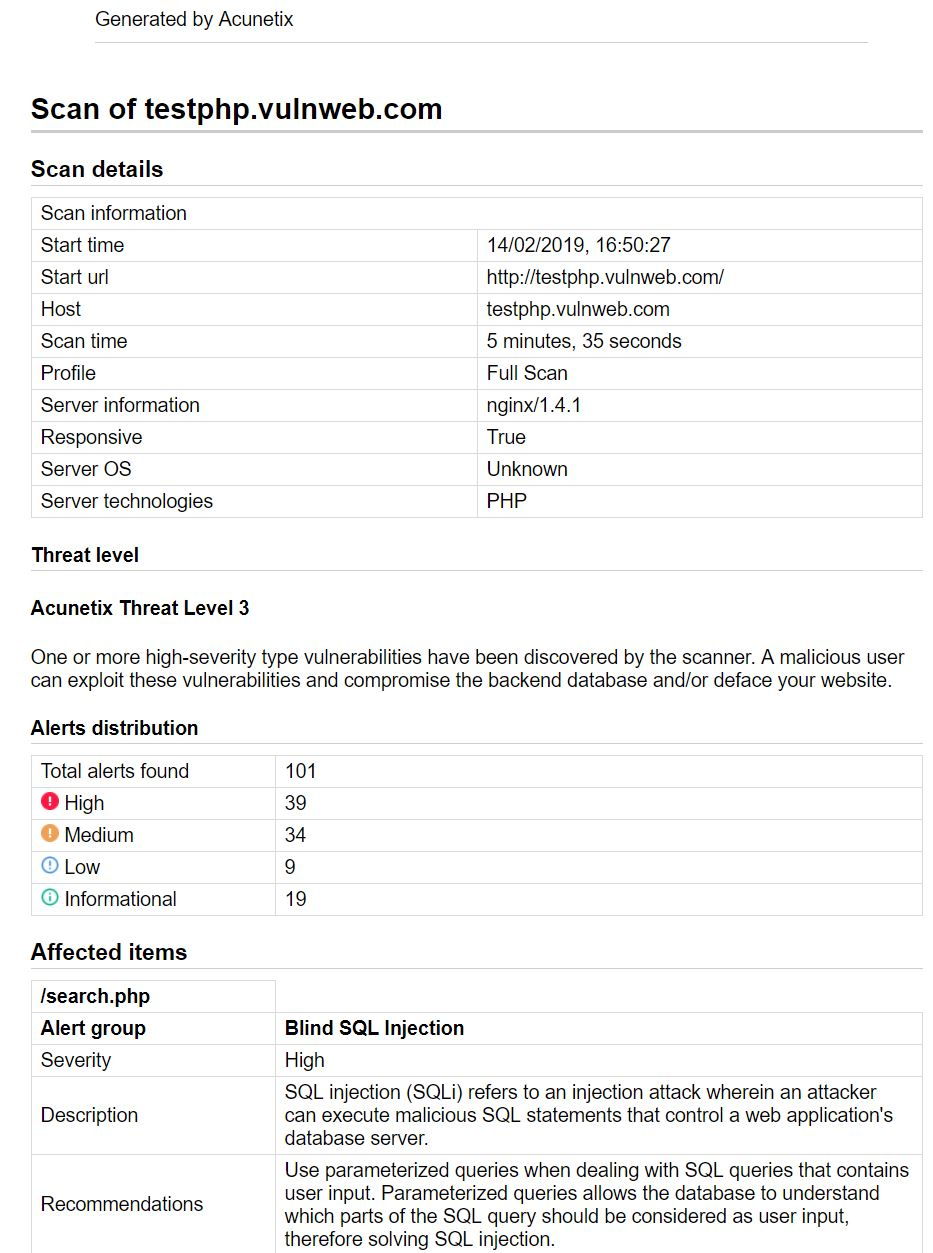
\includegraphics[width=0.8\textwidth]{Images/ScrAcunetix}
    \caption[Bericht Acunetix]{Bericht Acunetix}
  \end{figure}
  \begin{figure}[htb!]
    \centering
      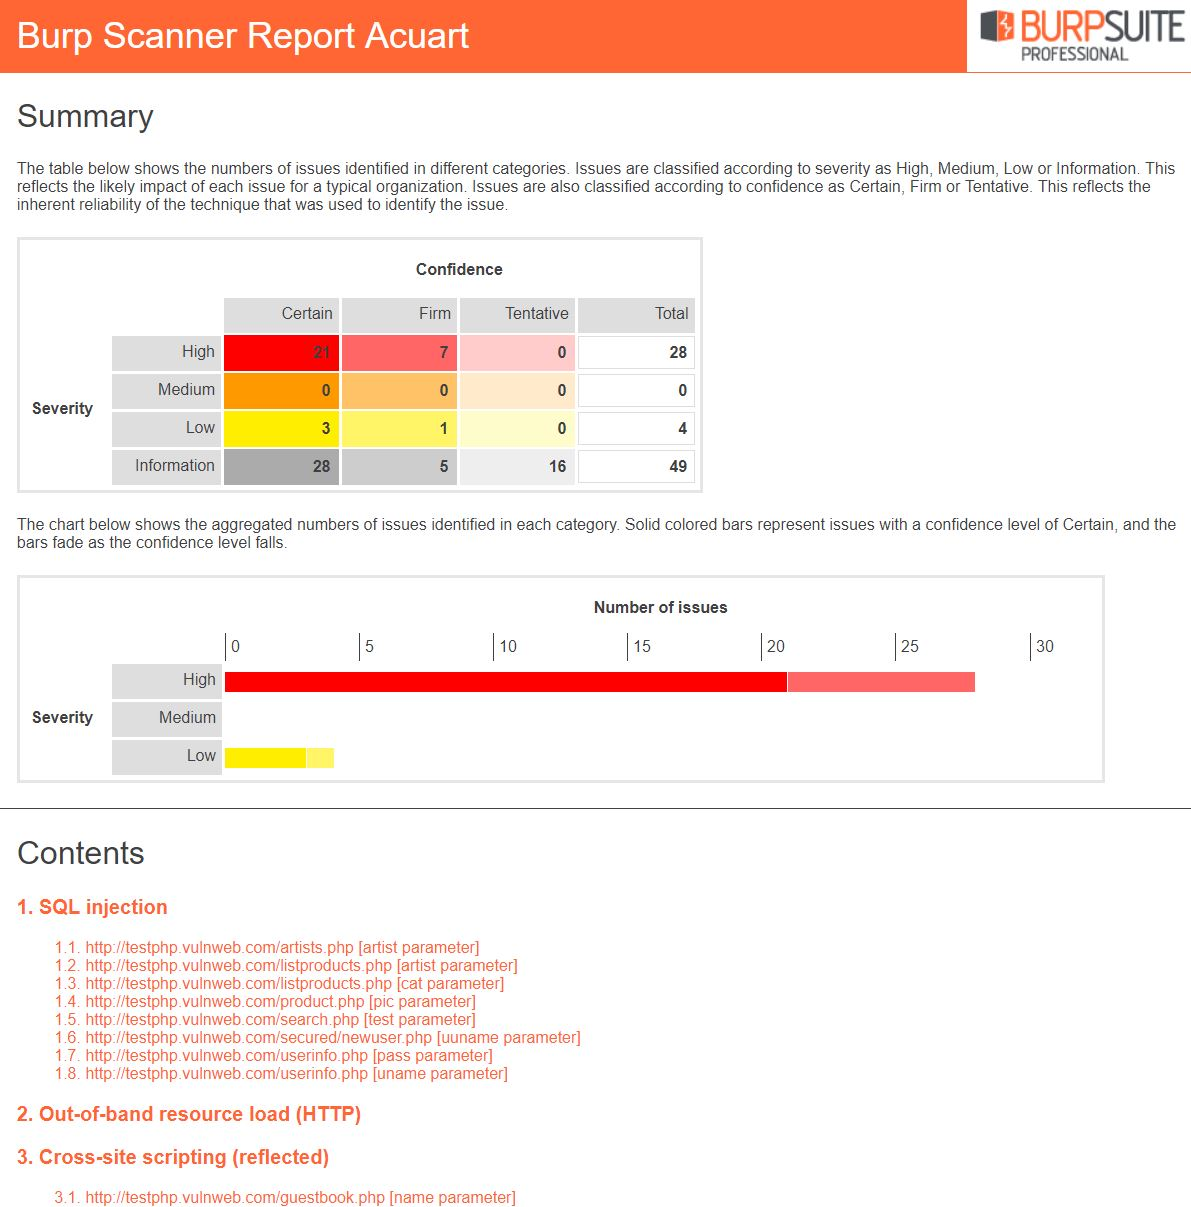
\includegraphics[width=1\textwidth]{Images/ScrBurp}
    \caption[Bericht BurpSuite Pro]{Bericht BurpSuite Pro}
  \end{figure}
  \begin{figure}[htb!]
    \centering
      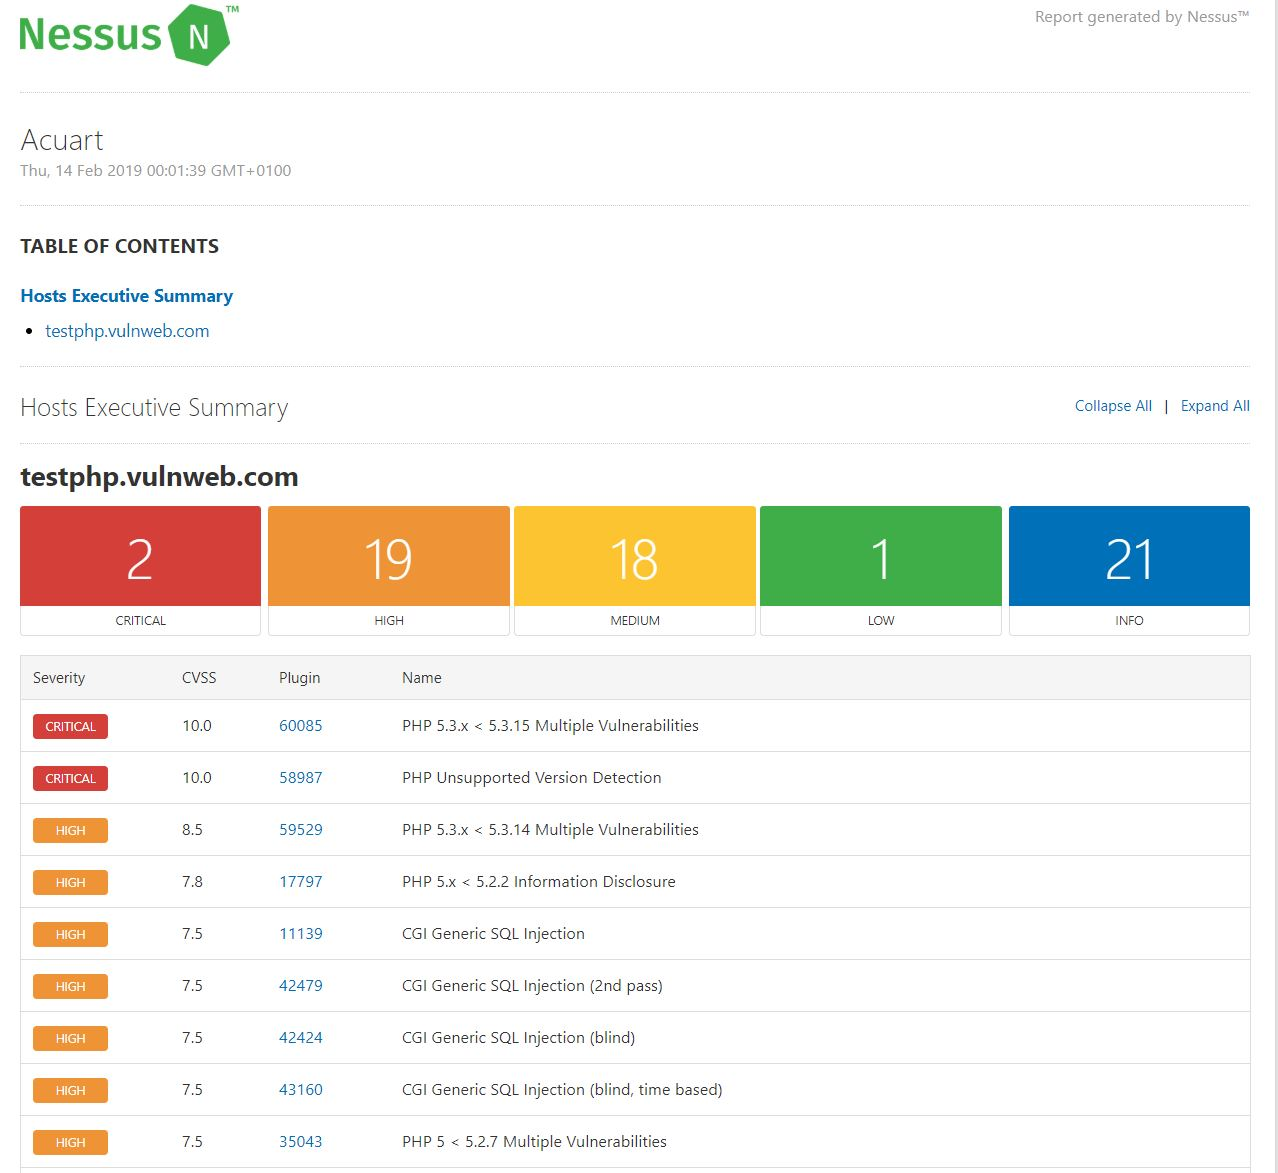
\includegraphics[width=1\textwidth]{Images/ScrNessus}
    \caption[Bericht Nessus]{Bericht Nessus}
  \end{figure}
  \begin{figure}[htb!]
    \centering
      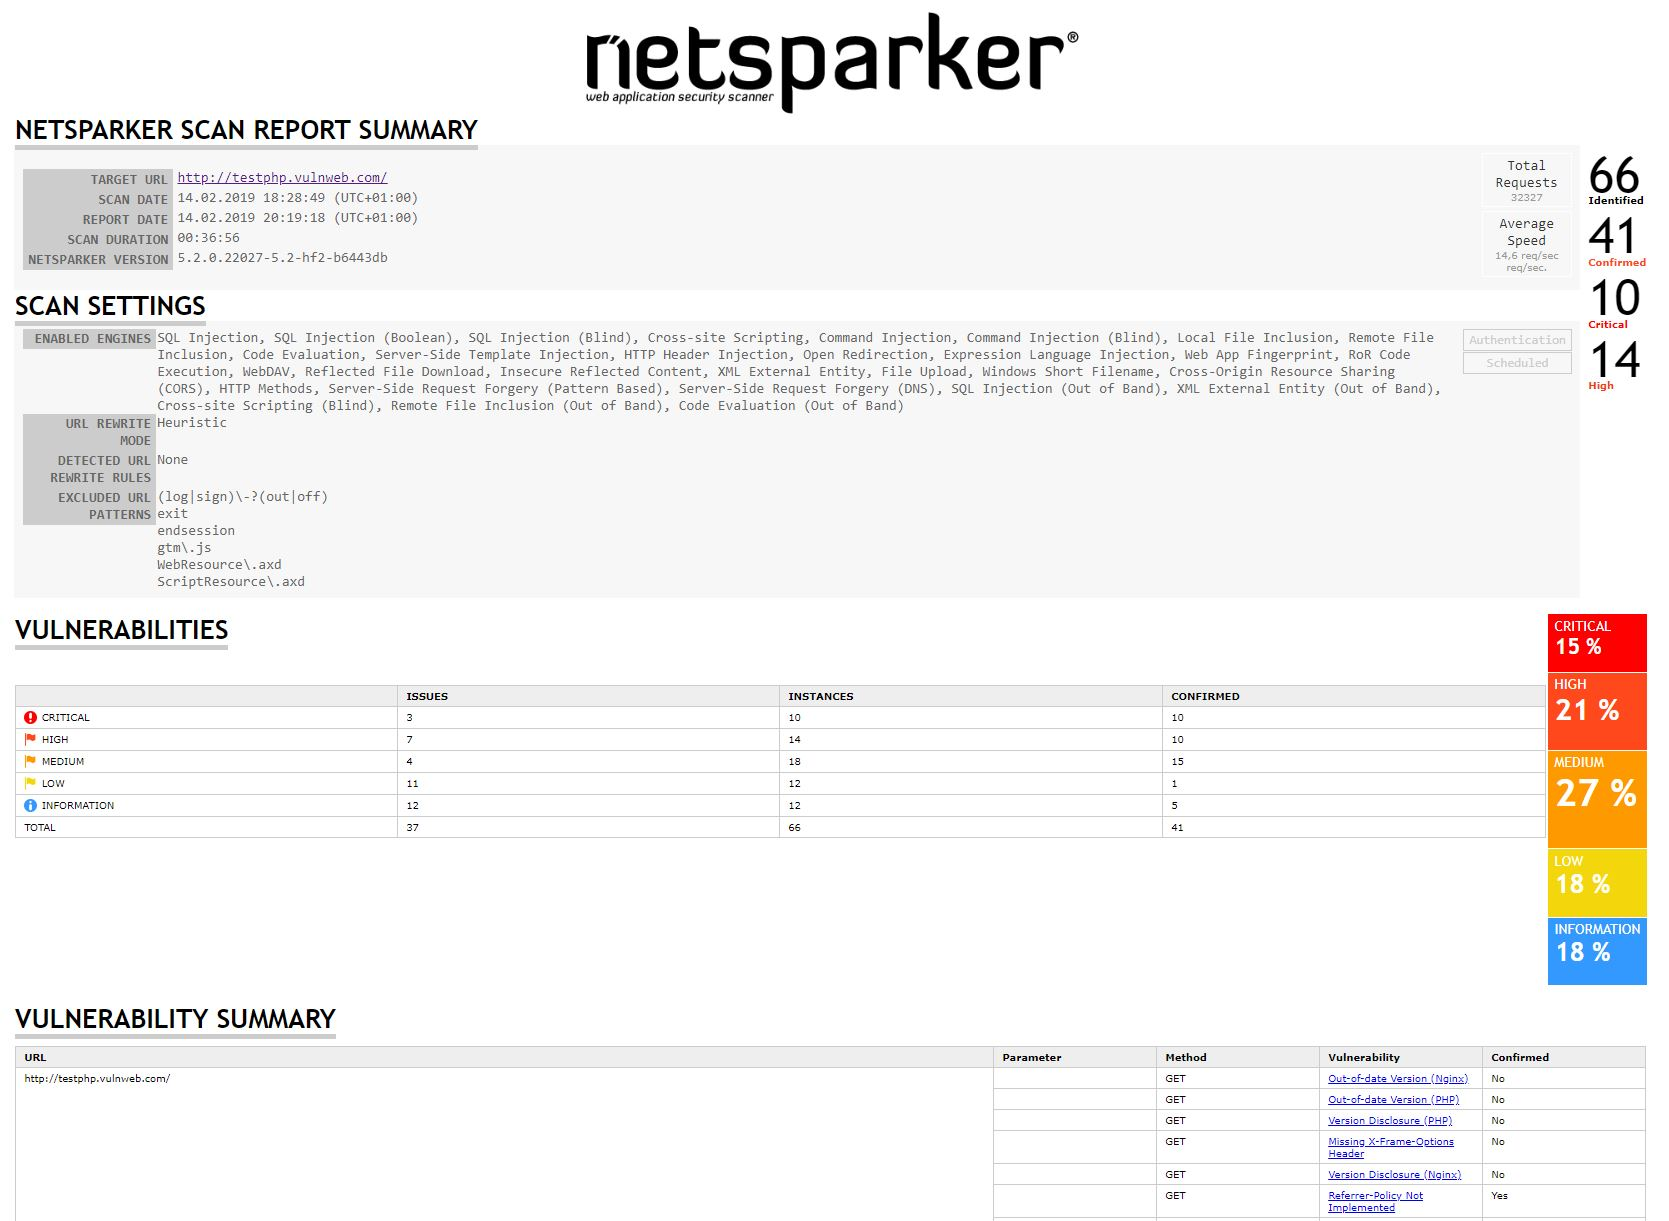
\includegraphics[width=1\textwidth]{Images/ScrNetsparker}
    \caption[Bericht Netsparker]{Bericht Netsparker}
  \end{figure}
  \begin{figure}[htb!]
    \centering
      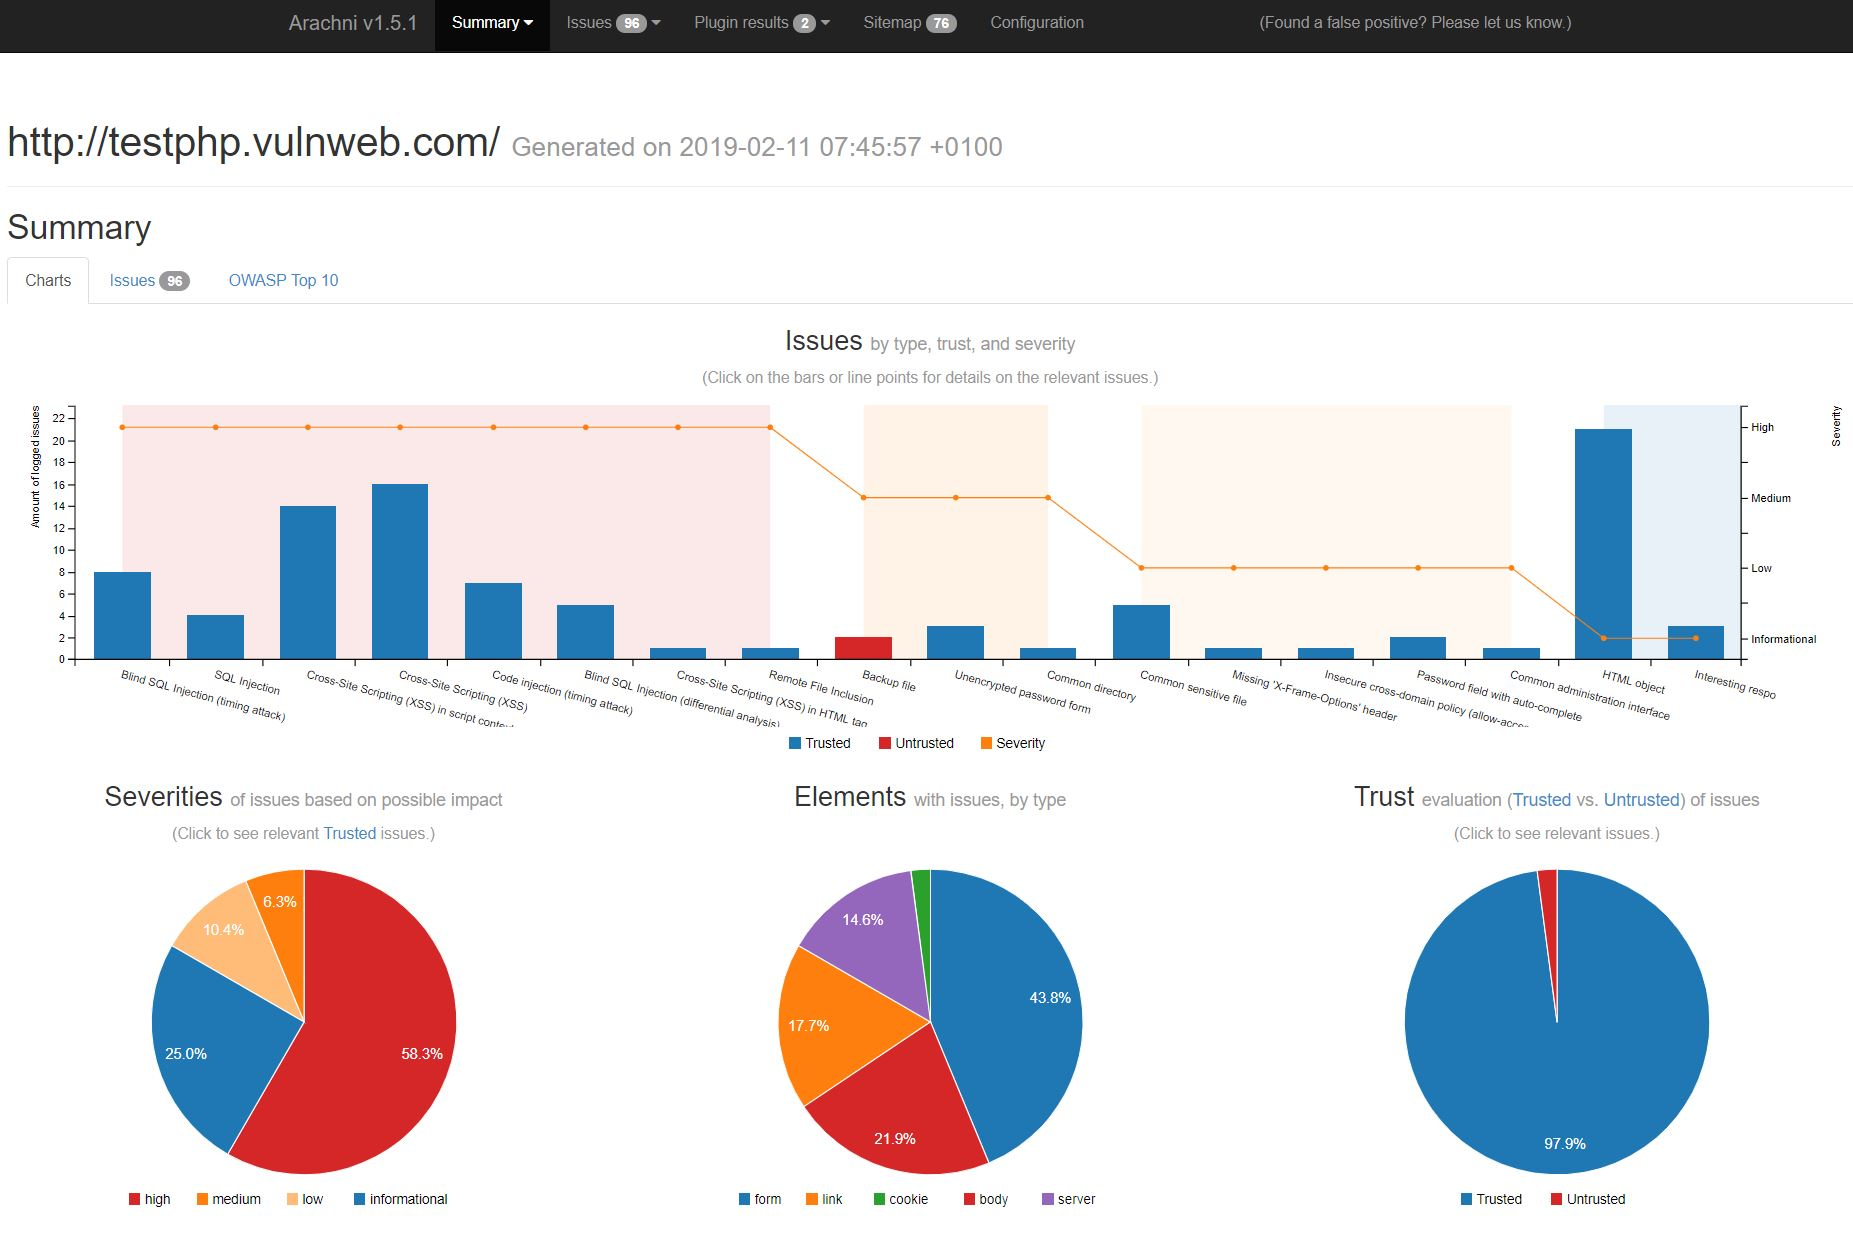
\includegraphics[width=1\textwidth]{Images/ScrArachni}
    \caption[Bericht Arachni]{Bericht Arachni}
  \end{figure}
  \begin{figure}[htb!]
    \centering
      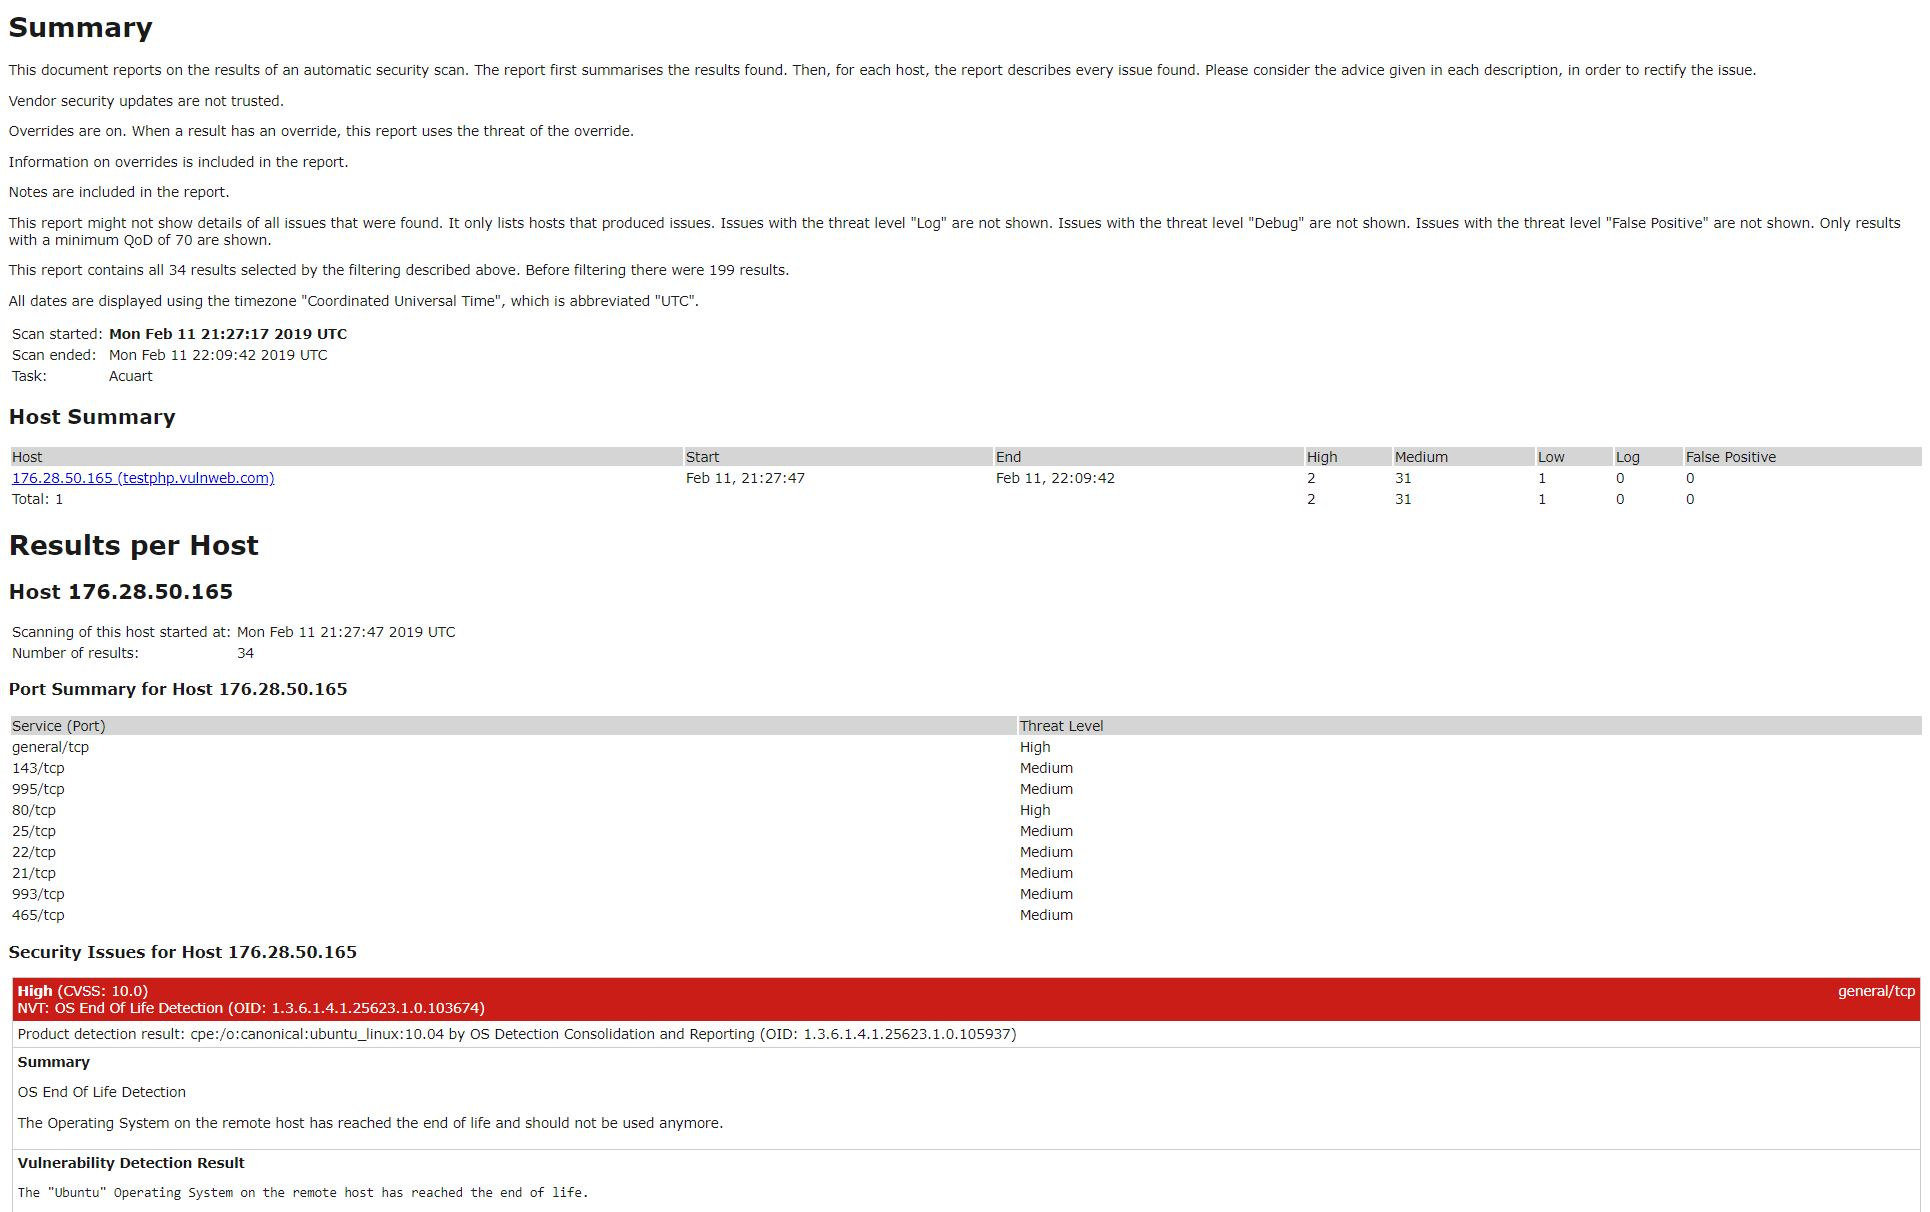
\includegraphics[width=0.9\textwidth]{Images/ScrOpenVAS}
    \caption[Bericht OpenVAS]{Bericht OpenVAS}
  \end{figure}
  \begin{figure}[htb!]
    \centering
      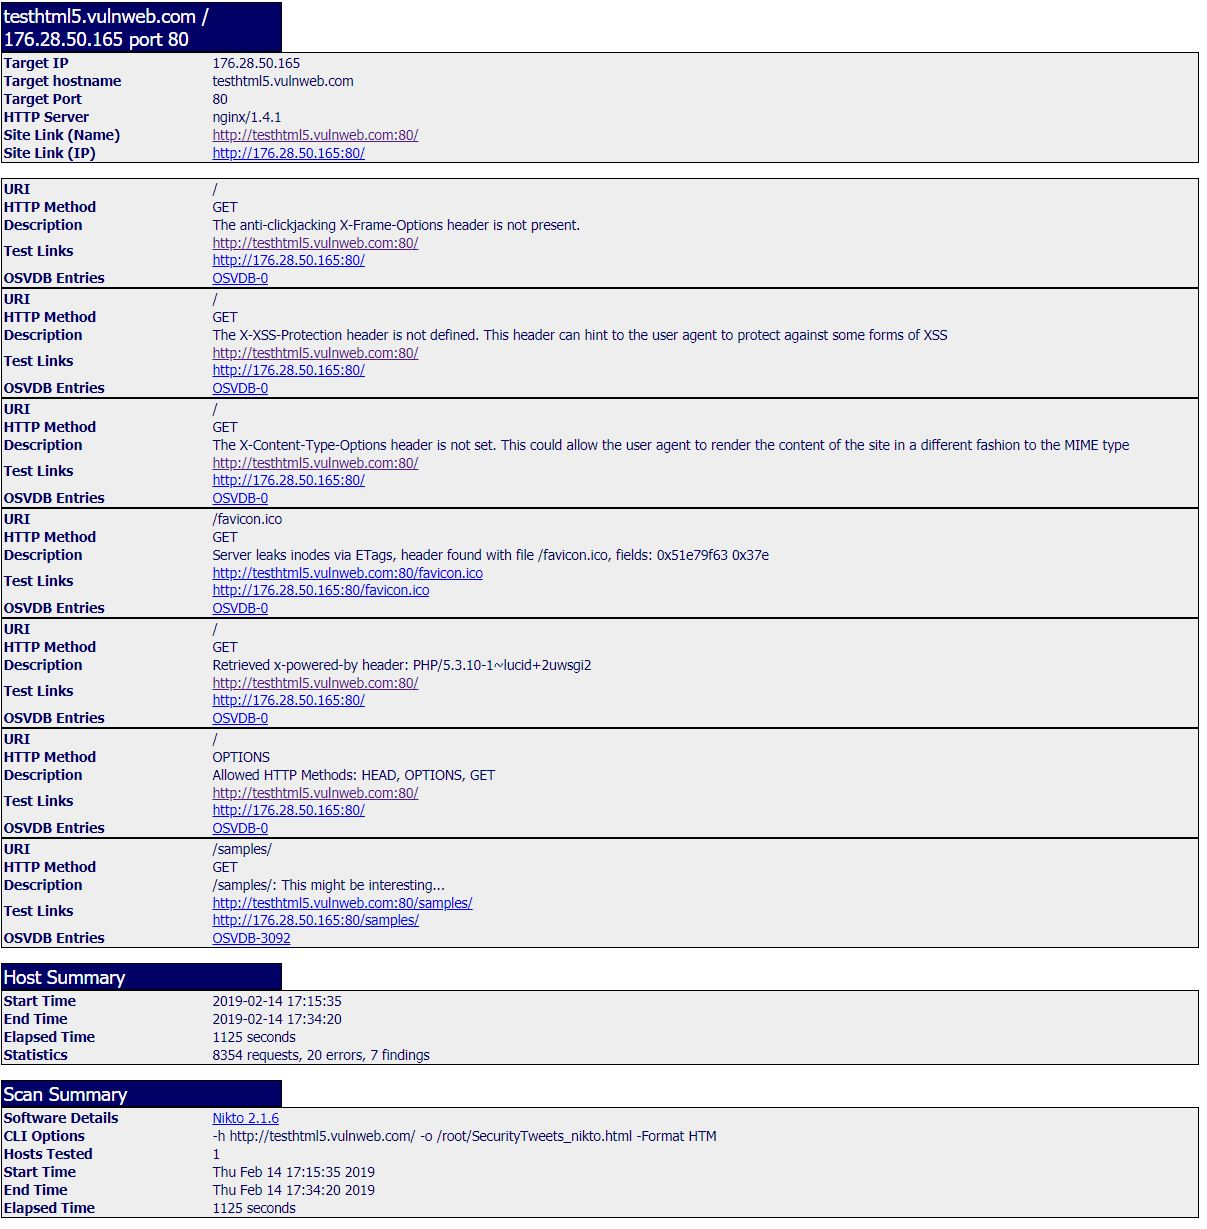
\includegraphics[width=1\textwidth]{Images/ScrNikto}
    \caption[Bericht Nikto]{Bericht Nikto}
  \end{figure}
  \begin{figure}[htb!]
    \centering
      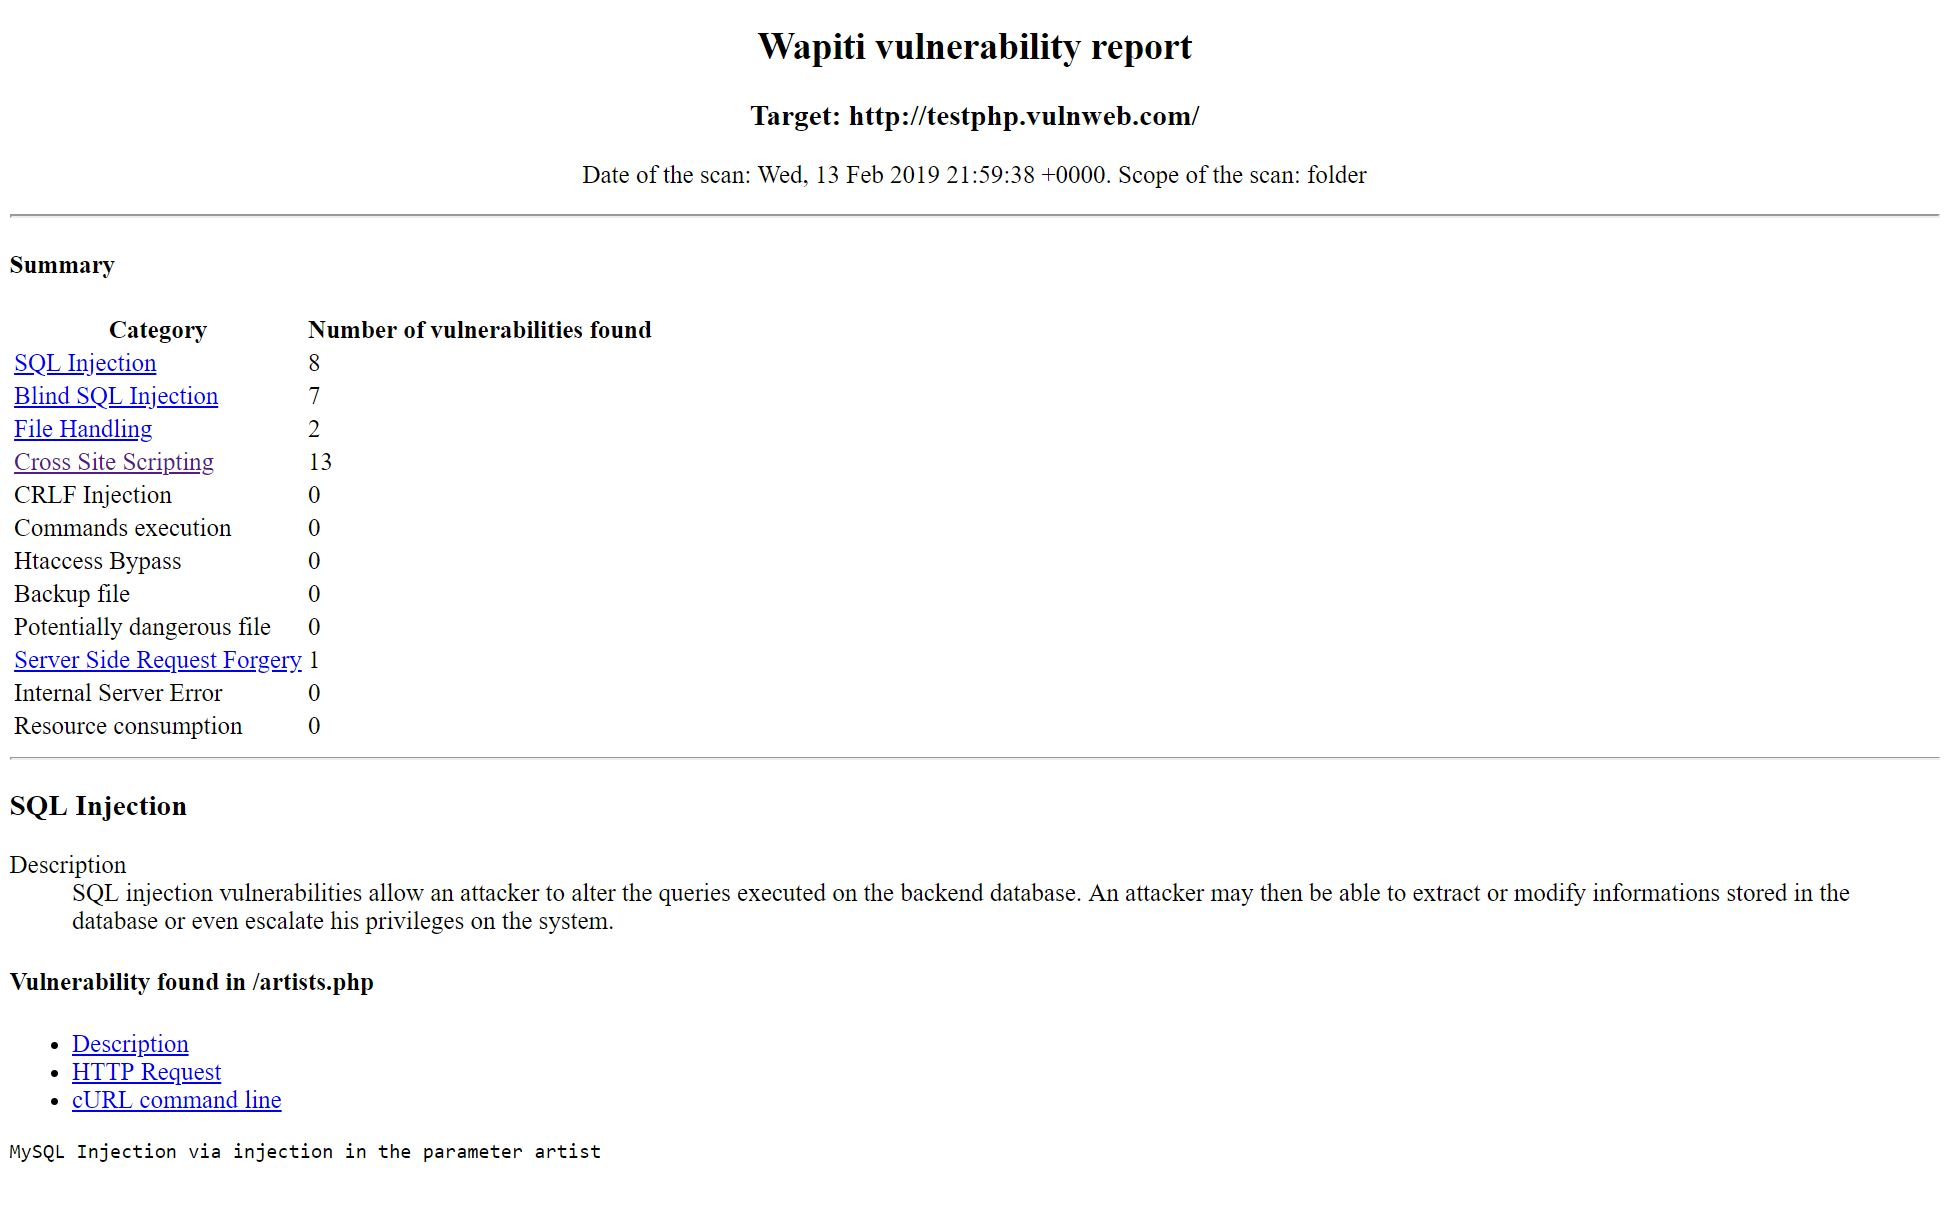
\includegraphics[width=1\textwidth]{Images/ScrWapiti}
    \caption[Bericht Wapiti]{Bericht Wapiti}
  \end{figure}
  \begin{figure}[htb!]
    \centering
      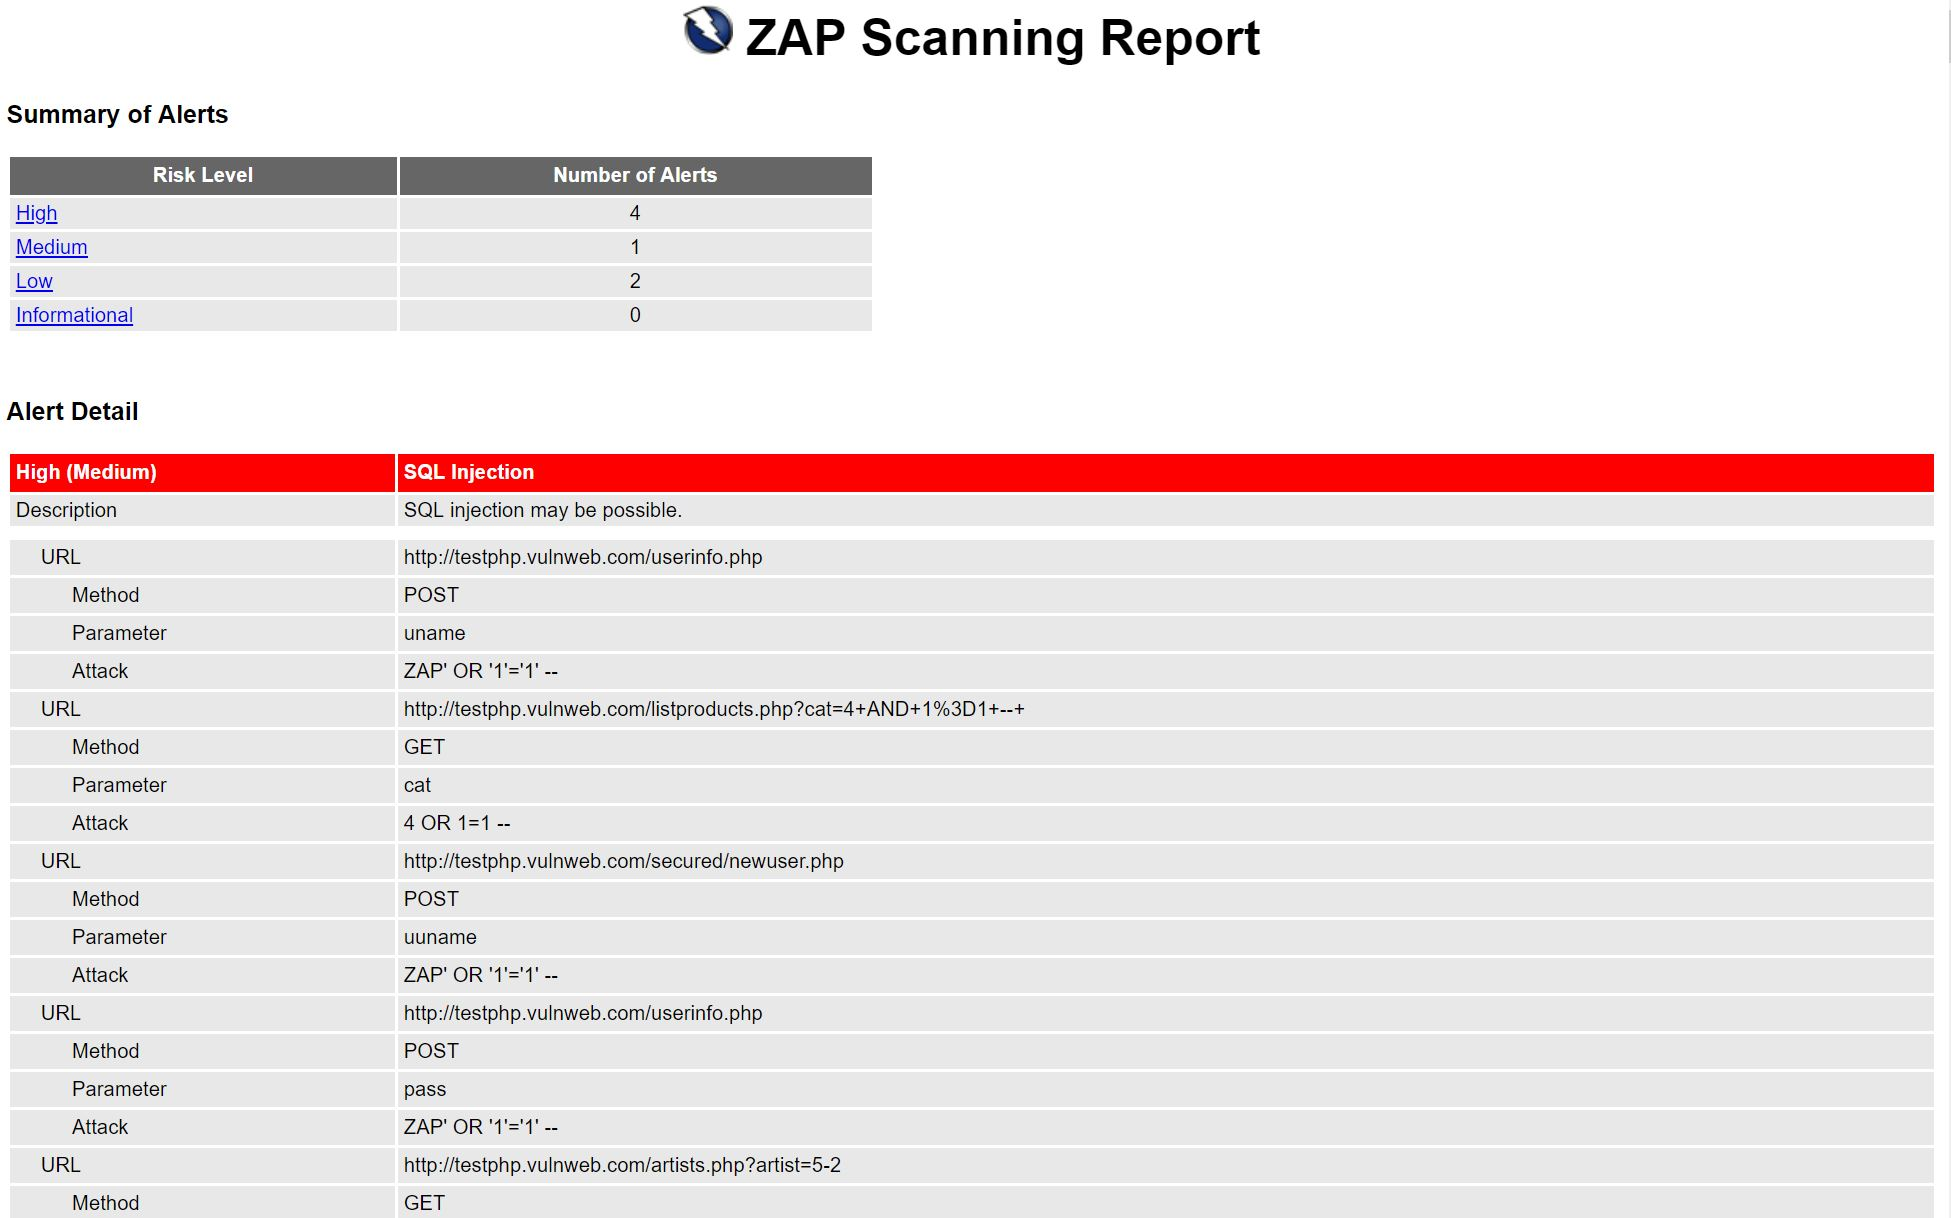
\includegraphics[width=1\textwidth]{Images/ScrZAP}
    \caption[Bericht ZAP]{Bericht ZAP}
  \end{figure}


\backmatter

%%%%%%%%%%%%%%%%%%%
%% declaration on oath
%%%%%%%%%%%%%%%%%%%
\addtocontents{toc}{\protect{\vspace{3ex}}}
\addchap{Eidesstattliche Erklärung}

Hiermit versichere ich, dass ich die vorgelegte Bachelorarbeit selbstständig verfasst und noch nicht anderweitig zu Prüfungszwecken vorgelegt habe. Alle benutzten Quellen und Hilfsmittel sind angegeben, wörtliche und sinngemäße Zitate wurden als solche gekennzeichnet.

\vspace{20pt}
Löwenstein, den \BaDeadline
\begin{flushright}
$\overline{~~~~~~~~~~~~~~~~~\mbox{\BaAuthor}~~~~~~~~~~~~~~~~~}$
\end{flushright}

\end{document}
